\documentclass[doc,a4paper,12pt]{apa6}
\usepackage[a4paper]{geometry}
\usepackage[utf8]{inputenc}
\usepackage[T1]{fontenc}
\usepackage[ngerman]{babel}
\usepackage{amsmath}
\usepackage[doublespacing]{setspace}
\usepackage{paralist}
\usepackage{graphicx}
\usepackage{epstopdf}
\usepackage{wrapfig}
\usepackage{float}
\usepackage{csquotes}
\usepackage[hidelinks]{hyperref}
\usepackage{pdfpages}
\usepackage[backend=biber,style=apa]{biblatex}
\usepackage[titles]{tocloft}
\usepackage{caption}
\usepackage{subcaption}

\hypersetup{hidelinks}
\usepackage{letltxmacro}
\makeatletter
\AtBeginDocument{%
  \@ifdefinable{\myorg@nameref}{%
    \LetLtxMacro\myorg@nameref\nameref
    \DeclareRobustCommand*{\nameref}[1]{%
      \glqq{\myorg@nameref{#1}}\grqq%
    }%
  }%
}
\makeatother

\DeclareLanguageMapping{ngerman}{ngerman-apa}
\DefineBibliographyStrings{ngerman}{andothers={et\ al\adddot}}

% spacing list
\setlength{\pltopsep}{1em}
% matrix/vector bold
\newcommand{\mx}[1]{\mathbf{#1}}
\renewcommand{\arraystretch}{1.2}

\bibliography{references}
 
\title{Intrinsische Rauschunterdückung bei LCMV Beamformer und Minimum Norm Estimate bei Magnetenzephalographie}
\shorttitle{Rauschunterdrückung bei LCMV Beamformer}
\author{Carlo Michaelis}
\date{12. August 2015}
%\affiliation{geb. am 29.09.1989 in Dieburg\\ Institut für Psychologie, Universität Leipzig\\ \ }

\renewcommand{\cftfigpresnum}{Abb. }
\settowidth{\cftfignumwidth}{Abb. 10\quad}

\geometry{a4paper, bottom=1.5in}
\setlength{\skip\footins}{1.5em}
\setlength{\footnotesep}{1.5em}
\setlength{\textfloatsep}{2em}
\raggedbottom

\begin{document}

%\maketitle

\thispagestyle{empty}

\begin{spacing}{1.1}
\begin{center}

\Large Universität Leipzig

\setlength{\parskip}{0.8em}
\normalsize Fakultät für Physik und Geowissenschaften

\setlength{\parskip}{6em}
\LARGE \textbf{Intrinsische Rauschunterdückung bei LCMV Beamformer und Minimum Norm Estimate bei Magnetenzephalographie}

\setlength{\parskip}{1.8em}
\normalsize Abschlussarbeit zur Erlangung des akademischen Grades\\ Bachelor of Science (B.Sc.)

\setlength{\parskip}{1.2em}
\normalsize vorgelegt von

\setlength{\parskip}{1.8em}
\Large \textbf{Carlo Michaelis}

\setlength{\parskip}{0.5em}
\normalsize geb. am 29.09.1989 in Dieburg

\setlength{\parskip}{3em}

Erstgutachter: Herr Dr. Burkhard Maess

\setlength{\parskip}{0.3em}
Zweitgutachter: Herr Prof. Dr. Jürgen Haase

\vfill

Dieses Dokument ist unter folgender Lizenz veröffentlicht:\\ \href{http://creativecommons.org/licenses/by-sa/4.0/}{Attribution-ShareAlike 4.0 International (CC BY-SA 4.0)}

\end{center}
\end{spacing}
\newpage

\section*{Selbstständigkeitserklärung}

Ich versichere hiermit, dass ich die vorliegende Arbeit selbständig verfasst und keine
anderen als die im Literaturverzeichnis angegebenen Quellen benutzt habe.\\
Alle Stellen, die wörtlich oder sinngemäß aus veröffentlichten oder noch nicht veröffentlichten
Quellen entnommen sind, sind als solche kenntlich gemacht.\\
Die Zeichnungen oder Abbildungen in dieser Arbeit sind von mir selbst erstellt worden oder
mit einem entsprechenden Quellennachweis versehen.\\
Diese Arbeit ist in gleicher oder ähnlicher Form noch bei keiner anderen Prüfungsbehörde
eingereicht worden.

\vspace{3em}
\noindent Leipzig, den XX.XX.2015\\ Carlo Michaelis

\newpage

\section*{Zusammenfassung}

Die Magnetenzephalographie ist ein hochpräzises Messverfahren zur Erfassung der magnetischen Aktivität im Gehirn. Diese Eigenschaft begünstigt eine hohe zeitliche Auflösung, birgt aber auch Nachteile, die sich vor allem in einer hohen Rauschanfälligkeit zeigen. Selbst wenn die Messbedingungen hochgradig optimiert werden, bleibt ein hoher Anteil von Störungen in den gemessenen Daten enthalten. Softwareseitige Rauschunterdrückungsverfahren wie die Signal Space Projection (SSP) oder die Signal Space Separation (SSS) können große Anteile des Rauschens eliminieren. In Folge dessen kann eine relativ präzise Lokalisation der Quellen im Gehirn mittels Dipolmodellen wie Minimum Norm Estimate oder räumlichen Filterverfahren wie Beamformer. Auf Grund bestimmter Eigenschaften des Linearly Constrained Minimum Variance (LCMV) Beamforming kann vermutet werden, dass das Lokalisationsverfahren an sich bereits Eigenschaften besitzt, die eine Unterdrückung des Rauschens ermöglichen. Gegenstand dieser Arbeit war es, herauszufinden, ob und in wie fern LCMV Beamformer diese Rauschunterdrückungseigenschaften besitzt. Im Vergleich wurden diese Eigenschaften auch für Minimum Norm Estimate untersucht. Im Ergebnis zeigte sich, dass beide Verfahren keine Eigenschaften zur Rauschunterdrückung besitzen, die eine Vorverarbeitung z.B. mittels SSP oder SSS überflüssig machen würden. Ferner konnte gezeigt werden, dass Minimum Norm Estimate grundsätzlich bessere Eigenschaften zur Lokalisation besitzt.

\newpage

\setcounter{tocdepth}{2}
\tableofcontents
\newpage

\listoffigures
\newpage

\section{Einleitung}

Auf dem Weg des Verstehens des eigenen menschlichen Geistes, kam es in den letzten Jahren - ca. seit Mitte der 1990er Jahre - zu einer beschleunigten Entwicklung von Verfahren und Methoden zur Messung der Gehirnaktivität, was seit dem zu einem deutlich besseren Verständnis der zerebralen Prozesse beigetragen hat. Vor allem der rasant zunehmenden und günstiger werdenden Computertechnologie ist es zu verdanken, dass heute Berechnungen möglich sind, die selbst vor 10 Jahren noch nahezu undenkbar waren. Es wird jedoch immer deutlicher, dass diese Entwicklung erst am Anfang steht. Neben der Erfassung zerebraler Aktivitäten - wie es in dieser Arbeit der Fall ist - wird es zunehmend auch zu Simulation von neuronalen Prozessen kommen, was durch den aktuellen Aufschwung künstlicher neuronaler Netzwerke, insbesondere durch Deep Learning derzeit deutlich wird \parencite[z.B.][]{ciresan2012multi}. Das zeigt, dass auch in den traditionellen Neurowissenschaften künftig deutlich komplexere Modelle verwendet werden können.

Bei der Untersuchung des Gehirns bilden die Quellorte und Aktivitäten (Dipolmomente) die zentralen Größen. Unterschiedliche Verfahren eigenen sich entsprechend ihrer Eigenschaften eher um Orte in hoher räumlicher Auflösung oder Aktivitäten in hoher zeitlicher Auflösung zu messen. Dabei werden im Folgenden nur nicht-invasiven Verfahren betrachtet. Eine Bildgebung, also die Bestimmung der Physiologie oder bei funktionellen Verfahren auch der physiologischen Quellen einer Aktivität mit möglichst hoher räumlicher Auflösung wird klassisch mit tomographischen Verfahren ermöglicht, z.B. Magnet-Resonanz-Tomographie~(MRT) und Computertomographie~(CT). Enzephalografische Verfahren sind hingegen auf eine hohe zeitliche Auflösung der zerebralen Aktivität spezialisiert. Zu diesen gehören Elektroenzephalographie~(EEG) und Magnetenzephalographie~(MEG).

Mit zunehmender Rechenkapazität und entsprechenden Modellen lassen sich inzwischen auch mit enzephalografischen Verfahren (z.B. EEG, MEG) die Quellen der Aktivität schätzen. Die Messung erfolgt dabei nur an der Oberfläche des Kopfes, eine Lokalisation erfolgt somit indirekt. Diese Verfahren haben den entscheidenden Vorteil, dass ihre zeitliche Auflösung meist so hoch ist, dass sie Veränderungen im Gehirn noch im Millisekundenbereich erfassen können. Zum Vergleich: Bildgebende funktionelle Verfahren, welche zusätzlich zur Bildgebung auch die Aktivität erfassen können - wie die funktionelle Magnet-Resonanz-Tomographie (fMRT) - liegen hier meist nur im Bereich von Sekunden. Auch wenn die enzephalografischen Verfahren in der zeitlichen Auflösung sehr gut sind, ihr Nachteil ist eine noch eher unpräzise Lokalisationsfähigkeit und eine hohe Verrauschung der Daten. Während die Messgrößen bei MEG im Bereich von Femto-Tesla liegen, ist selbst der Herzschlag am Gehirn noch im Bereich von Picotesla messbar. Netzstrom mit $50\,Hz$ und die Schwingung des Bahnnetzes mit $16,67\,Hz$, sowie deren Harmonische sind beispielsweise am Standort des Max-Planck-Insituts für kognitive Neurowissenschaften in Leipzig trotz starker Abschirmung deutlich messbare Größen in jeder MEG-Messung (siehe auch Abschnitt \nameref{sec:rauschen} auf Seite \pageref{sec:rauschen}). Die Frequenzen der genannten Artefarkte in den Rohdaten lassen sich mit Hilfe einer Fourier-Analyse abschätzen, wie in Abbildung~\ref{img:freq-analy} auf Seite~\pageref{img:freq-analy} dargestellt.

Verschiedene Faktoren beeinflussen folglich die Messung, die niemals unter idealen Bedingungen statt findet. Es liegen unterschiedliche Möglichkeiten der Vermeidung und Unterdrückung vor. Während der Hersteller des verwendeten Gerätes \emph{Vectorview} (Elekta Neuromag, Elekta Oy, Helsinki, Finland) das Programm \emph{MaxFilter} als Teil der \emph{Neuromag}-Software mit liefert, mit der versucht wird zwischen äußeren und inneren Quellen zu trennen (siehe Abschnitt \nameref{sec:maxfilter} auf Seite \pageref{sec:maxfilter}), soll es Ziel dieser Bachelorarbeit sein die Robustheit verschiedener Verfahren gegenüber den angesprochenen Rauschgrößen zu erproben. Dabei werden die Verfahren mit und ohne voriger Verwendung von MaxFiter gegenübergestellt.

Die Hypothese soll lauten, dass das Quellrekonstruktionsverfahren Beamformer relativ stabil gegenüber Rauschen sein müsste und eine Anwendung softwareseitiger Rauschunterdrückungsverfahren nicht nötig ist, um eine gute Lokalisation zu erreichen, während das Quellrekonstruktionsverfahren Minimum Norm Estimate ohne vorherige Anwendung von Rauschunterdrückungsverfahren eher zu unpräziseren Ergebnissen führen sollte. Die Hypothese wird im entsprechenden Abschnitt auf Seite \pageref{sec:hypo} formuliert und begründet.

Im Folgenden werden zunächst die Grundlagen zur Biologie, zum Messverfahren und Rauschen erläutert. Anschließend soll im Abschnitt \nameref{sec:hinter} auf die Quelllokalisation und die dafür benötigten Modelle eingegangen werden. Im Abschnitt \nameref{sec:methodik} ab Seite \pageref{sec:methodik} wird dann beschrieben wie die formulierte These geprüft wurde. Das Ergebnisse wird dann im Abschnitt \nameref{sec:ergebnisse} und \nameref{sec:diskussion} ab den Seiten \pageref{sec:ergebnisse} bzw. \pageref{sec:diskussion} vorgestellt und diskutiert werden.

% #################################
% ##### GRUNDLAGEN BIOLOGISCH #####
% #################################

\subsection{Biologische Grundlagen}

\subsubsection{Kopf- und Gehirnstruktur}
\label{sec:head-struct}

Der Kopf als Träger des Gehirns besteht aus mehreren Komponenten, welche zum messtechnischen Verständnis von großer Relevanz sind. Die Kopfoberfläche (head shape) bzw. Kopfhaut (scalp) ist der äußerste Bereich. An diesem liegen bei EEG- und MEG-Messungen die Sensoren zur Messung an (bzw. ca. $2\,cm$ darüber). Unterhalb der Kopfoberfläche befindet sich der Schädelknochen (skull), welcher das darin liegende Gehirn schützt. Das Gehirn wiederum ist von einer Bindegewebsschichten umgeben, der Hirnhaut. Die Gehirnmasse selbst, lässt sich grob in zwei Bereiche einteilen, die graue Substanz und die weiße Substanz. Während die graue Substanz eine hohe Dichte an Zellkörpern und eher weniger myelinisierte Axone enthält, enthält die weiße Substanz entsprechend viele lange und myelinisierte Axone und eher weniger Zellkörper. Im Gehirn liegt die graue Substanz eher in äußeren Bereichen und umhüllt die weiße Substanz. Die beiden groben Typen der Gehirnmasse weisen unterschiedliche messtechnische Eigenschaften auf, so ist die Leitfähigkeit der grauen Substanz isotrop, während die der weißen Substanz anisotrop ist \parencite{logothetis2007vivo}.

\subsubsection{Elektrische und magnetische Eigenschaften der Nervenzellen}

Alle Nervenzellen des Körpers kommunizieren durch kleine elektrische Ströme. Dabei können zwei unterschiedliche Arten der elektrischen Aktivität unterschieden werden \parencite{da1998biophysical}. Die \emph{postsynaptischen Potentiale} und die u.U. daraus resultierenden \emph{Aktionspotentiale}. Im Gleichgewicht besitzen Nervenzellen ein \emph{Ruhepotential} im Bereich von ca. $-70\,mV$. Graduelle lokale Änderungen des Membranpotentials werden als \emph{exzitatorisches postsynaptisches Potential} (EPSP) bezeichnet, wenn sie zur Auslösung eines Aktionspotentials beitragen. \emph{Inhibitorische postsynaptisches Potential} (IPSP) bezeichnen im Gegensatz graduelle Potentialveränderungen, die der Auslösung eines Aktionspotentials entgegenwirken. Wird an der Zellmembran ein bestimmter Potentialschwellwert, der bei ca. $-55\,mV$ liegt, überschritten, so kommt es zu einer beschleunigten Ausschüttung von Ionen. Der in Folge auftretende Ionenstrom resultiert in einer starken Potentialverschiebung auf bis zu $+20\,mV$ bis $+30\,mV$ führt. Das Aktionspotential dauert jedoch nur ca. $1$-$2\,ms$ und wird während seiner Ausbreitung über mehrere Nervenzellen schnell wieder abgedämpft. Da zusätzlich die Wahrscheinlichkeit für eine präzise synchrone Ausbreitung sehr gering ist, ist die Messung der elektrischen und magnetischen Felder eines Aktionspotential sehr unwahrscheinlich. Was hingegen gut erfasst werden kann sind die postsynaptischen Potentiale, welche die Ursache für ein Aktionspotential bilden können. Die Potentiale breiten sich - verglichen mit dem Aktionspotential - langsamer und gleichmäßiger über größere Nervenzellen-Strukturen aus. Die von ihnen verursachten elektrischen und magnetischen Felder können an der Oberfläche, d.h. außerhalb der Kopfhaut, gemessen werden.

\subsubsection{ERP und ERF}
\label{sec:erf}

Das \emph{ereigniskorrelierte Potential} (event-related potential, ERP) bezeichnet ein elektrisches Potential, welches im Gehirn auftritt und mit einem EEG detektiert werden kann \parencite{luck2014introduction}. Es tritt leicht verzögert mit einem bestimmten Ereignis in der Umwelt auf. Bei MEG-Messungen wird der Begriff des \emph{ereigniskorrelierten Feldes} (event-related field, ERF) verwendet \parencite{brown1999neurocognition}.

Ein klassisches Beispiel eines ERP bzw. ERF ist die MMN, die so genannte \emph{Mismatch Negativity}. Das Ereignis ist in diesem Fall die Änderung eines zuvor geregelten Stimulus. Werden z.B. hinreichend viele Töne gleicher Höhe, Länge und Lautstärke am gleichen Ohr abgespielt und folgt dann eine Änderung des Stimulus, z.B. andere Höhe, Länge, Lautstärke oder eine Präsentation am anderen Ohr, so folgt auf dieses Ereignis eine Änderung des elektrischen Potentials im Gehirn bzw. eine Änderung des magnetischen Feldes im Gehirn im Abstand von ca. $150$-$250\,ms$ zum Stimulus. Das experimentelle Design, welches eine einfache Abweichung unter vielen gleichen Stimuli  vorsieht, wird als \emph{Oddball-Paradigma} bezeichnet \parencite{squires1975two,naatanen1989event,paavilainen1991right}. Das Ereignis (\glqq anderer Ton\grqq) ist korreliert mit dem Auftreten eines Potentials (ERP) bzw. eines Feldes (ERF) im Gehirn, der MMN \parencite{naatanen1978early} oder MMNm als äquivalent magnetischer Messungen.

\subsubsection{Auditorischer Kortex}
\label{sec:audicort}

\begin{figure}[t]
%  \centering
%  \captionsetup{justification=centering}
  %
  \begin{subfigure}[c]{0.47\textwidth}
    \fbox{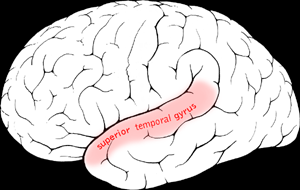
\includegraphics[width=\textwidth]{einleitung/stg.png}}
    \subcaption{Gyrus temporalis superior (STG), enthält den auditorischen Kortex.\\ Verwendet von \glqq Auditory cortex\grqq .\\ (18. März 2015). In Wikipedia, The Free Encyclopedia. Abgerufen 19:47, 04. August 2015, von \url{https://en.wikipedia.org/w/index.php?title=Auditory_cortex&oldid=653871107}}
    \label{img:gyrustemp}
  \end{subfigure}\hspace*{0.04\textwidth}
  %
  \begin{subfigure}[c]{0.47\textwidth}
    \fbox{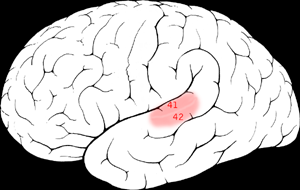
\includegraphics[width=\textwidth]{einleitung/brodmann-41-42.png}}
    \subcaption{Auditorischer Kortex in den Brodmann Arealen 41 und 42.\\ Verwendet von \glqq Superior temporal gyrus\grqq.\\ (20. Juli 2015). In Wikipedia, The Free Encyclopedia. Abgerufen 19:57, 04. August 2015, von \url{https://en.wikipedia.org/w/index.php?title=Superior_temporal_gyrus&oldid=672262435}}
    \label{img:audicort}
  \end{subfigure}
  %
  \vspace*{3mm}
  \caption{Gyrus temporalis superior (STG) und auditorischer Kortex}
  \label{img:audi}
\end{figure}

Der auditorische Kortex ist ein bestimmter Bereich des Gehirns. Er befindet sich an den Brodmann Arealen 41 und 42, dargestellt in Abbildung~\ref{img:audicort}. Der auditorische Kortex ist Teil des Gyrus temporalis superior~(STG) in Abbildung~\ref{img:gyrustemp}, welcher bei jeglicher auditiver Stimulation aktiviert wird \parencite{binder1994functional}. Im auditorischen Kortex erfolgt dann das Bewusstwerden akustischer Signale \parencite{jaaskelainen2004human}.

In den vorliegenden Daten handelt es sich um ein auditives Experiment, weshalb die ERF bzw. konkret die MMNm im auditorischen Kortex erwartet werden.

% ###########################
% ##### GRUNDLAGEN MEG  #####
% ###########################

\subsection{Grundlagen der Magnetenzephalographie}

Das MEG (Magnetenzephalographie) misst die magnetischen Aktivität des Gehirns. Es ist das zweitjüngste Verfahren zur Messung der Gehirnströme. Nachdem in den 1920er Jahren das EEG durch Hans Berger entwickelt und 1929 erstmals publiziert wurde \parencite{berger1929elektrenkephalogramm}, folgte das MEG erst 1968 \parencite{cohen1968magnetoencephalography}, war damit aber noch vor anderen Verfahren zur Vermessung des Gehirns, wie dem CT (Computertomographie) oder dem MRT (Magnet-Resonanz Tomographie). Trotzdem ist das MEG auf Grund seiner hohen Empfindlichkeit, seiner damit verbundenen hohen Rauschanfälligkeit und ebenso auf Grund seines noch unausgeschöpften Lokalisationspotentials auch heute noch ein Verfahren welches sich in einem kontinuierlichen Optimierungsprozess befindet.

Da die Kosten eines MEG deutlich über denen eines EEG liegen, stellt sich die berechtigte Frage warum überhaupt die magnetische Komponente der Nervenzellen-Aktivität gemessen wird, zumal Ergebnisse aus EEG-Messungen mit denen aus MEG-Messungen weitestgehend vergleichbar sind \parencite{huotilainen1998combined}. Zusätzlich lassen sich mit MEG nur die tangentialen Komponenten der Aktivität messen, während EEG sowohl tangentiale, als auch radiale Aktivität erfassen kann. Die Vorteile des MEG liegen jedoch in einer geringeren Störung der magnetischen Signale durch den Schädel und die Kopfhaut, und einer damit verbundenen höheren räumliche Auflösung. Während das EEG also mehr Aktivität erfassen kann, ist das MEG präziser in der Erfassung und ermöglicht eine genauere Lokalisation. Zusätzlich sind die zeitliche Auflösung unterhalb einer Millisekunde~$\Delta t < 10^{-3}\,s$, die hohe Anzahl der Kanäle und die genaue Kenntnis über die Position der Kanäle (auf Grund des starren MEG-Helms) wichtige Vorteile des MEG zur Lokalisation der Quellen  \parencite{malmivuo2012comparison}.

\subsubsection{SQUIDs}
\label{sec:squids}

Technische Grundlage der Magnetenzephalographie bilden SQUIDs (Superconducting Quantum Interference Device, dt.: Supraleitende Quanteninterferenzeinheit), welche 1964 in den Ford Research Labs entwickelt wurden \parencite{jaklevic1964quantum}. Sie basieren auf dem Josephson Effekt, der bereits 1962 von Brian D. Josephson vorhergesagt wurde \parencite{josephson1962possible}. Josephson sagte voraus, dass zwei Supraleiter, welche durch eine wenige Nanometer dicke nicht-supraleitende Schicht getrennt werden (Josephson-Kontakt) und mit einem geringen elektrischen Strom durchflossen werden, von Cooper-Paaren derart durchtunnelt werden können, dass sich der Josphson-Kontakt wie ein unterbrechungsfreier Supraleiter verhält. Die Cooper-Paare tunneln in dem Fall widerstandsfrei.
Auf Grund der Cooper-Paare sind die Wellenfunktion zweier Elektronen gekoppelt (abhängig von der Dicke der Schicht). Mit den Wellenfunktionen $\Psi_1$, $\Psi_2$ und den Hamilton-Operatoren $H_1$, $H_2$, sowie dem Kopplungskoeffizienten $T$ gilt:

\begin{subequations}
\label{eq:cooper}
  \begin{equation} i\hbar \frac{\partial \Psi_1}{\partial t} = H \Psi_1 + T \Psi_2 \label{eq:cooper1}\end{equation}
   \begin{equation} i\hbar \frac{\partial \Psi_2}{\partial t} = H \Psi_2 + T \Psi_1 \label{eq:cooper2}\end{equation}
\end{subequations}

Die erste Josphson-Gleichung (Gleichung \ref{eq:joseph}) beschreibt die Abhängigkeit des Stroms im Supraleiter $I_S$ vom kritischen Strom $I_0$, wobei $\Delta \phi$ die Phasendifferenz zwischen den zwei Wellengleichungen \ref{eq:cooper1} und \ref{eq:cooper2} bezeichnet.

\begin{equation}
\label{eq:joseph}
I_S = I_0\,\sin{\Delta \varphi}
\end{equation}

Die Josphson-Gleichung gilt jedoch nur für Prozesse ohne Magnetfeld. Sobald ein Magnetfeld anliegt, muss die Gleichung korrigiert werden. Es liegt eine Abhängigkeit des Strom im Supraleiter $I_S$ vom anliegenden Magnetfeld $\vec{B}$ bzw. vom zugehörigen magnetischen Vektorpotential $\vec{A}$ vor:

\begin{equation}
\label{eq:josephfeld}
I_S = I_0\,\sin{\left( \Delta \varphi - \frac{2\pi}{\Phi_0} \int_{S1}^{S2} \vec{A}\,d\vec{l} \right)}
\end{equation}

Der zweite Term ergänzt Gleichung \ref{eq:joseph} um ein Wegintegral vom ersten Supraleiter $S1$ über den Josephson-Kontakt zum zweiten Supraleiter $S2$. $\Phi_0$ entspricht dem Flussquant (siehe auch Gleichung \ref{eq:flussquant}).

Ein SQUID basiert auf diesem Prinzip und enthält zwei Josephson-Kontakte, in welchem ein Gleichsstrom fließt (DC SQUID) oder einen Josephson-Kontakt, in welchem ein Wechselstrom fließt (RF SQUID). Die Leiter in einem SQUID sind zu einem Ring zusammengeschlossen. Entscheidend ist, dass sich der Strom innerhalb des SQUID abhängig vom äußeren Magnetfeld verhält, wie in Gleichung \ref{eq:josephfeld} gezeigt. Das anliegende Magnetfeld kann auf einzelne Flussquanten genau angegeben werden. Ein Flussquant entspricht:

\begin{equation}
\label{eq:flussquant}
\Phi_0 = \frac{h}{2e} \approx 2,068\,Tm^2
\end{equation}

Die magnetische Flussdichte der Gehirnaktivität liegt im Bereich von wenigen $10^{-15}\,T$ und kann daher nur mit hochsensiblen Sensoren gemessen werden. Zum Einsatz kommen daher SQUIDs.

\subsubsection{Flux-Transformator}

\begin{figure}[t]
  \centering
  \setlength{\fboxsep}{8mm}
  \fbox{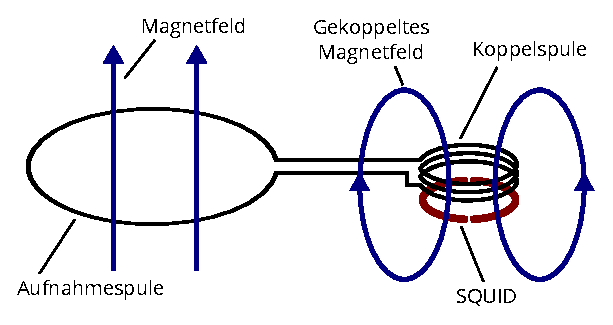
\includegraphics[width=0.6\textwidth]{einleitung/koppelspule.eps}}
  %
  \vspace*{3mm}
  \caption[Prinzip eines Flux-Transformators]{Prinzip eines Flux-Transformators. An der Aufnahmespule wird vom magnetischen Feld ein Strom induziert. Die Koppelspule erzeugt ein äquivalentes magnetisches Feld in unmittelbarer Nähe des SQUID.}
  \label{img:flux-trafo}
\end{figure}

Um die Signale zu erfassen wird ein \emph{Flux-Transformator} eingesetzt, welcher das Signal an einen SQUID weiterleitet. Der Flux-Transormator wird so nah wie möglich an den Kopf der Versuchsperson gebracht (im Bereich von ca.~$2\,cm$). Ein vom Gehirn der Versuchsperson erzeugtes magnetisches Feld erzeugt an einer Aufnahmespule einen Strom. Dieser wird über eine Koppelspule wieder in ein äquivalentes Magnetfeld zurückgeführt. Die Koppelspule befindet sich in unmittelbarer Nähe des SQUID an dem das Signal letztlich messbar wird. Der Sachverhalt ist in Abbildung~\ref{img:flux-trafo} dargestellt. Der Flux-Transformator wird in zwei verschiedenen Varianten verwendet, dem Magnetometer und dem Gradiometer.

\subsubsection{Magnetometer und Gradiometer}

Magnetometer besitzen nur einen Ring an der Aufnahmespule des Flux-Transformators, sie messen den absoluten Wert der magnetischen Flussdichte in radiale Richtung $B_z$ in $T$. Neben der hohen Sensitivität gegenüber nahen Quellen, wie magnetische Aktivität im Gehirn, erfassen Magnetometer auch Signale aus weiter Entfernung und damit ungewünschte Aktivität aus der Umgebung \parencite{hansen2010meg}. Beispielsweise erreicht ein fahrendes Auto in $2\,km$ Entfernung eine Signalstärke, die mit dem der Gehirnaktivität äquivalent ist \parencite{weinstock2012squid}.

Gradiometer besitzen zwei entgegengesetzt angebrachte Ringe an der Aufnahmespule des Flux-Transformators. Die zwei Ringe eines Gradiometers können axial oder planar angeordnet sein. Die zwei Ringe messen einen räumlichen Gradienten. Der Gradient der magnetische Flussdichte $G_x = dB_z/dx$ bzw. $G_y = dB_z/dy$ wird in $T/m$ angegeben. Die Annahme ist, dass weit entfernte Quellen ein relativ homogenes Feld erzeugen. Da die zwei Aufnahmespulen des Gradiometers mit einem entgegengesetzten Strom durchflossen werden und die gemessenen magnetischen Flussdichten voneinander subtrahiert werden, verschwindet der Gradient für weit entfernte Quellen im Idealfall, so dass nur nahe Quellen erfasst werden \parencite{hansen2010meg}.

Im Falle des verwendeten MEG-Systems (\emph{Vectorview}, Elekta Neuromag, Elekta Oy, Helsinki, Finland) enthält jeder der 102 Sensoren drei Kanäle mit einem Magnetometer und zwei Gradiometern.

\subsection{Artefakte und Rauschen}

Wie bereits im Abschnitt \nameref{sec:squids} auf Seite \pageref{sec:squids} deutlich wurde, ist das MEG ein äußerst empfindliches Messinstrument, welches im Bereich einzelner Flussquanten $\Phi_0$ messen kann. Ziel ist es nur die Gehirnsignale zur weiteren Berechnung zu verwenden und alle anderen Störfaktoren auszuschließen. Dafür kann eine Reihe von Maßnahmen getroffen und entsprechende Software eingesetzt werden, die im Folgenden erläutert wird.

\subsubsection{Allgemeine Rauschunterdrückung}
\label{sec:rauschen}

Prinzipiell können unterschiedliche Artefakte und Rauschfaktoren ausgemacht werden. Grob können drei Bereiche klassifiziert werden: (1) Umwelt, (2) Versuchsperson und (3) Messtechnik.

Am besten zu beeinflussen ist der Faktor der Umwelt (1). Innerhalb von Städten ist beispielsweise viel bewegtes Metall (z.B. Autos, Straßenbahnen), welches zu allgemein schwachen, aber im MEG deutlich messbaren Magnetfeldern führt. Zusätzliche treten viele periodische elektrische und magnetische Felder auf (z.B. Netzkabel, Oberleitungen). All diese Faktoren können durch eine entsprechende Standortwahl deutlich verringert werden. Die verbleibenden Faktoren können durch ein stark geschirmten Messraum weiter verringert werden. Verbleibende Faktoren sind meist trotzdem deutlich in den Messungen sichtbar (z.B. Netzkabel im Gebäude).

Auch die Versuchsperson (2) hat einen großen Einfluss auf die Messung. Bewegung der Augen, Herzschläge und Kopfbewegungen, allgemein jede Kontraktion eines Muskels, führt zu deutlich messbaren mehr oder weniger periodischen Artefakten. Durch ein gutes Versuchsdesign und eine professionelle Einweisung können einige dieser Faktoren verringert werden, letztlich ist die Disziplin der Versuchsperson jedoch der entscheidende Faktor.

Letztlich hat auch die Messtechnik (3) in Form klassischen Rauschens einen entscheidenden Einfluss, maßgeblich durch Sensorrauschen.

\textcite{vigario1998independent} und \textcite{vigario2000independent} fassten mit Hilfe einer ICA (Independent Component Analysis) die wichtigsten Faktoren für Rauschen und Artefakte bei MEG-Messungen zusammen. Es ergaben sich folgende allgemeine Faktoren für Artefakte der Versuchsperson~(2):

\begin{compactitem}
\item Gebiss-Muskulatur
\item Horizontale Augenbewegung und Blinzeln
\item Herzmuskel
\item Atmung
\end{compactitem}

\subsubsection{Softwareseitige Rauschunterdrückung}
\label{sec:maxfilter}

Nachdem das Rauschen bereits während der Messung versucht wird so gut wie Möglich zu unterdrücken, kann auch auf Softwareebene nachgearbeitet werden. Eine Möglichkeit bietet die \emph{Signal-space projection}~(SSP), für die eine Leerraummessung notwendig ist. Eine andere rechenintensivere Möglichkeit bietet die proprietäre Software MaxFilter von Neuromag (siehe auch Abschnitt \nameref{sec:software} auf Seite \pageref{sec:software}), die \emph{Signal-Space Separation}~(SSS) zur Trennung äußerer und innerer Quellen anwendet. Mit \emph{Movement Correction}~(MC) können zusätzlich die Bewegungen der Versuchsperson nachträglich korrigiert werden.

Der Signalraum (signal-space) ist ein $n$-dimensionaler Raum, wobei~$n$ der Anzahl der Kanäle entspricht. Ein Vektor bzw. ein Punkt im Signalraum entspricht einem vollständigen Signal zu einem Zeitpunkt. Das räumliche Muster des Signals entspricht der Richtung des Vektors, die Intensität des Signals entspricht dem Betrag des Vektors \parencite{hansen2010meg}.

SSP wurde Ende der 90er Jahre von \textcite{uusitalo1997signal} und \textcite{parkkonen1999interference} entwickelt. Die Methode basiert auf dem Vorliegen einer Leerraummessung. In einer kurzen Messung werden die üblichen magnetischen Aktivitäten im Messraum aufgezeichnet, ohne dass eine Versuchsperson anwesend ist. Das Ergebnis entspricht den Umweltartefakten, die als stationär angenommen werden und zu jeder späteren Messung vorhanden sind. Wird eine Messung mit Versuchsperson durchgeführt, so bildet die Leerraummessung einen Unterraum des gewöhnlichen Signalraums. Durch eine orthogonale Projektion des Signalraums auf den Unterraum der Leerraumessung, ergibt sich ein weiterer Unterraum, der die Signale ohne die Umwelteinflüsse enthalten sollte. Jegliche äußeren Artefakte werden damit entfernt oder zumindest drastisch reduziert.

SSS wurde wenige Jahr später von \textcite{taulu2004suppression} und \textcite{taulu2005presentation} entwickelt. Dabei wird das gemessene Magnetfeld in einer Reihenentwicklung beschrieben. Jedes Potentialfeld $V(\mx{r})$ kann beschrieben werden mit:

\begin{equation}
V(\mx{r}) = \sum_{l=1}^\infty \sum_{m=-l}^l \alpha_{lm} \frac{Y_{lm}(\Theta, \varphi)}{r^{l+1}} + \sum_{l=1}^\infty \sum_{m=-l}^l \beta_{lm} r^l Y_{lm}(\Theta, \varphi) 
\label{eq:sss-pot}
\end{equation}

Die Entwicklung in der ersten Summe ist im Ursprung singulär, in der zweiten Summe divergiert sie für unendliches~$l$. $Y_{lm}$~ist die normalisierte harmonische Funktion mit den sphärischen Koordinaten~$\Theta, \varphi$ und~$r$:

\begin{equation}
Y_{lm}(\Theta, \varphi) = \sqrt{\frac{2l+1}{4\pi} \frac{(l-m)!}{(l+m)!}}\, P_{lm}(\cos{\Theta})\,e^{im\varphi}
\end{equation}

Wobei $P_{lm}(\cos{\Theta})$ Legendre-Polynome sind. Die magnetische Flussdichte kann analog entwickelt werden:

\begin{equation}
\mx{B}(\mx{r}) = \sum_{l=1}^\infty \sum_{m=-l}^l \alpha_{lm} \mx{a}_{lm} + \sum_{l=1}^\infty \sum_{m=-l}^l \beta_{lm} \mx{b}_{lm}
\label{eq:sss-magpot}
\end{equation}

Die Vektoren $\mx{a}_{lm}$ und $\mx{b}_{lm}$ entsprechen den Termen $Y_{lm}(\Theta, \varphi)/r^{l+1}$ und $r^l Y_{lm}(\Theta, \varphi)$ aus Gleichung~\ref{eq:sss-pot}. $\Phi$~kann als Signalvektor interpretiert werden. Bezeichne~$n$ weiterhin die Anzahl der Kanäle, dann bilden~$n$ linear unabhängige Signalvektoren~$\Phi$ den Signalraum. Die SSS-Methode basiert auf diesem Koordinatensystem. Es gilt:

\begin{equation}
\Phi = \mx{S}\,\mx{x} = \left( \mx{S}_{\text{innen}}, \mx{S}_{\text{außen}} \right) \left( \mx{x}_{\text{innen}} \atop \mx{x}_{\text{außen}} \right)
\end{equation}

$\mx{S}_{\text{innen}}$ und $\mx{S}_{\text{außen}}$ werden mit den Basen $\mx{a}_{lm}$ und $\mx{b}_{lm}$ beschrieben, während $\mx{x}_{\text{innen}}$ und $\mx{x}_{\text{außen}}$ von $\alpha_{lm}$ und $\beta_{lm}$ beschrieben werden. Mit Hilfe des aufgestellten Koordinatensystems kann eine räumliche Filterung vorgenommen werden, die in zwei Aspekten von Bedeutung ist:

\begin{compactitem}
\item Vollständig unkorrelierte Signale, wie Artefakte an einzelnen Kanälen oder zufälliges Rauschen der Gerätekomponenten werden sowohl von Termen mit niedrigen, wie auch von Termen mit hohen Indizes beschrieben. Signale von realen Quellen sind in Termen mit hohen Indizes nicht mehr vertreten. Wird die Reihenentwicklung abgebrochen, sobald der Beitrag der realen Quellen nicht mehr relevant ist, kann ein Großteil des Rauschens und der Artefakte, welches auf messtechnischer Ebene entsteht, herausgefiltert werden.
\item Man kann zeigen, dass externe Quellen außerhalb des MEG-Helms mit den Termen in der zweiten Summe von Gleichung~\ref{eq:sss-magpot} zusammenhängen. Umgekehrt sind Signale, welche vom Inneren des MEG-Helmes (respektive vom Gehirn) stammen mit den Termen der ersten Summe verknüpft. Intuitiv wird dies in Gleichung~\ref{eq:sss-pot} deutlich. Der erste Term enthält - wie bereits angesprochen - eine Singularität im Ursprung, die zweite Summe divergiert für unendlich große~$l$. Durch einfaches Weglassen der zweiten Summe werden die Einflüsse der externen Quellen deutlich verringert.
\end{compactitem}

Beide Summen zusammen erklären die gesamt vorkommende Aktivität bzw. approximieren die gesamte vorkommende Aktivität für endliche Glieder. Anschaulich erklärt jedoch die erste Summe die Aktivität von innen nach außen. Daher ist es sinnvoll hier nur eine begrenzten Anzahl an Termen zu verwenden. Die zweite Summe erklärt die Aktivität von außen nach innen, weshalb dieser ganz weggelassen werden kann, da hier fast ausschließlich äußere Aktivität zu erwarten ist.

Die SSS-Methode ist zwar deutlich rechenaufwändiger als SSP, führt jedoch im Gegenzug zu deutlich rauschfreieren Ergebnissen. Zusätzlich ist keine Leerraummessung notwendig. Die Methode kann durch die angesprochene Movement Correction (MC) erweitert werden. Im normalen SSS-Verfahren wird angenommen, dass die Versuchsperson während eines Durchgangs bzw. Blocks unbewegt sitzen bleibt. Die Kopfpositionen werden nur zwischen den Blöcken auf die Position zu Beginn der gesamten Messung korrigiert. Bei der zusätzlichen MC-Berechnung wird die Kopfposition für jeden Zeitpunkt korrigiert. Zur Erfassung der Kopfposition sind Spulen am Kopf angebracht, welche zu jedem Zeitpunkt die Position der Versuchsperson erfassen. Eine zusätzliche nachträgliche Korrektur der Kopfposition ist vor allem dann sinnvoll, wenn sich die Versuchsperson sehr viel bewegt hat. Die Notwendigkeit dieses Rechenschritts kann mit Bewegungsprofilen abgeschätzt werden.

% ####################################
% ##### GRUNDLAGEN LOKALISATION  #####
% ####################################

\newpage
\section{Hintergrund zur Quelllokalisation}
\label{sec:hinter}

Die Messung der magnetischen Signale erfolgt ausschließlich über die außerhalb des Kopfes befindlichen Sensoren. Die entscheidende Frage ist also: Wie ist es möglich anhand der magnetischen Signale außerhalb des Gehirns auf die physiologischen Quellen innerhalb des Gehirns zu schließen? Um diese Frage zu beantworten wird zunächst etwas Theorie eingeführt und anschließend das Vorwärtsmodell, sowie verschiedene Methoden zur Schätzung der Lösung des inversen Problems erläutert.

% ###########################
% ##### VORWÄRTSMODELL  #####
% ###########################

\subsection{Grundlagen und Vorwärtsmodell}

\subsubsection{Superposition}

Jede Quelle im Gehirn wirkt auf alle Sensoren an der Kopfoberfläche, jeder Sensor empfängt also Signale jeder einzelnen Aktivität im Gehirn. Es liegt eine Superposition der Quellaktivität vor, wie sie in Abbildung \ref{img:superposition} dargestellt ist. Ähnlich einer Unterhaltung mit 10 sprechenden Personen und 5 aufnehmenden Mikrofonen. Jedes Mikrofon empfängt aus einer anderen Perspektive alle 10 Gespräche. Wünschenswert wäre es nun ein einzelnes Gespräch zu isolieren \emph{und} zu lokalisieren. Übertragen auf das Gehirn soll versucht werden die Quellen der Aktivitäten zu identifizieren und deren spezifische Aktivitäten über die Zeit zu erhalten. Die Quellen werden durch Dipole beschrieben und diskretisiert. Entsprechend soll für jeden angenommenen Dipol an einem bestimmten Ort im Gehirn ein Aktivitätsverlauf über die Zeit berechnet werden.

\begin{figure}
  \centering
%  \captionsetup{justification=centering}
  %
    \setlength{\fboxsep}{8mm}
  \fbox{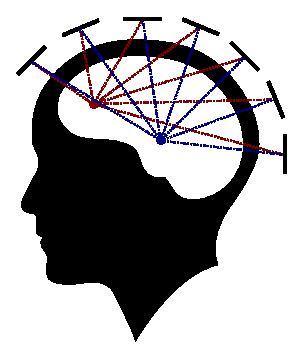
\includegraphics[width=0.5\textwidth]{einleitung/superposition.eps}}
  %
  \vspace*{3mm}
  \caption[Superposition der Quellaktivität an den Sensoren]{Superposition der Quellaktivität an den Sensoren. Die schwarzen Balken symbolisieren die Sensoren, der rote und der blaue Punkt bilden jeweils eine Quelle, deren Signale gestrichelt zu den Sensoren führen. An jedem Sensor liegen die Aktivitätsinformationen aller Quellen vor.\\ Das Kopf-Icon wurde über \url{http://www.flaticon.com} bereitgestellt und von \url{http://www.freepik.com} erstellt. Das Aktivitätsmuster, die Sensoren und die Linien der Signale wurden ergänzt.}
  \label{img:superposition}
\end{figure}

\subsubsection{Segmentierung und Volumenleiter}
\label{sec:segment}

Die Quellbestimmung ist nur an bestimmten Stellen innerhalb des Kopfes wirklich sinnvoll, außerhalb des Gehirns ist bspw. keine elektrischen Stromdipole zu erwarten. Außerdem ist es wünschenswert die Aktivität im Gehirn nicht auf eine standardisierte mathematische Form (z.B. auf eine Kugel) zu berechnen, sondern ein echtes Gehirn zu verwenden, im Idealfall das tatsächliche Gehirn der entsprechenden Versuchsperson. Dafür muss zunächst ein bildgebendes Verfahren eingesetzt werden. Üblicherweise eignet sich dafür ein MRT-Scan des Kopfes.

Das Bild des Kopfes enthält zunächst noch keine Informationen über physiologische Bestandteile. Mit dem Softwarepaket \emph{Freesurfer} kann das Bild des Kopfes in seine Segmente zerlegt werden (siehe auch \nameref{sec:head-struct} auf Seite \pageref{sec:head-struct}). Es wird unterschieden zwischen der Kopfoberfläche bzw. Kopfhaut, dem Schädel und dem Gehirn. Innerhalb des Gehirns werden graue und weiße Substanz getrennt.

\begin{figure}[t]
  \centering
%  \captionsetup{justification=centering}
  %
  \fbox{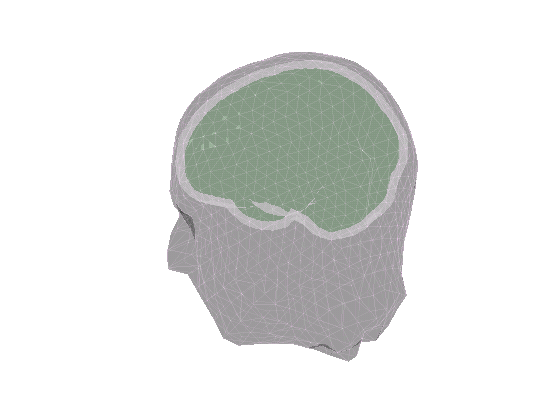
\includegraphics[width=0.6\textwidth]{einleitung/bem.png}}
  %
  \vspace*{3mm}
  \caption[Volumenleiter, berechnet mittels Boundary Element Model (BEM)]{Volumenleiter, berechnet mittels Boundary Element Model (BEM). Darstellung der drei segmentierten Bereiche: Gehirn (grün), Schädel (weiß), Kophaut (grau).\\ Verwendet von \glqq Creating a volume conduction model of the head for source-reconstruction of EEG data\grqq . (01. April 2015). In FieldTrip wiki. Abgerufen 15:02, 10. August 2015, von \url{http://www.fieldtriptoolbox.org/tutorial/headmodel_eeg}}
  \label{img:bem}
\end{figure}

Anschließend wird ein Kopfmodell (Head Model) berechnet, welches die verschiedenen Gewebetypen beinhaltet. Dafür können numerische Verfahren wie z.B. das \emph{Boundary Element Model} (BEM) verwendet werden. Das BEM-Verfahren modelliert die Ränder der segmentierten Volumina mit Dreiecksflächen. Dabei wird angenommen, dass die Leitfähigkeit innerhalb des Volumens isotrop ist. Dies stellt eine Idealisierung da. Im Abschnitt \nameref{sec:head-struct} auf Seite \pageref{sec:head-struct} wurde bereits deutlich, dass eine vollständige homogene Leitfähigkeit nicht der Realität entspricht. Die graue Substanz, die sich vor allem an der zu betrachtenden Oberfläche befindet, kann damit jedoch sehr gut genähert werden.

Die Diskretisierung der Oberfläche im BEM-Modell wirkt sich auf die Quellrekonstruktion aus. Wird die Dichte der Netzpunkte zu gering gewählt kommt es zu Fehlern in der numerischen Berechnung, die Quellen werden fehlerhaft geschätzt. Die Seitenlängen der Dreiecke sollten unterhalb von $10\,mm$ liegen. Zusätzlich sollte das Verhältnis von Dipoltiefe zur Seitenlänge der Dreiecke nicht kleiner als $0,5$ sein \parencite{haueisen1997effect}. Die Anzahl der Netzpunkte muss entsprechend hoch genug gewählt werden.

Im Gegensatz zum BEM-Modell wird im FEM-Modell (\emph{Finite Element Model}) das gesamte Volumen modelliert. Im FEM-Modell können demnach auch Bereiche mit anisotroper Leitfähigkeit berücksichtigt werden. Dies entspricht mehr der Realität und lohnt sich vor allem bei einer Lokalisation, welche auch das innere des Gehirns berücksichtigt, da die weiße Substanz mit ihrer anisotropen Leitfähigkeit präziser modelliert werden kann.

Nach der Berechnung des Kopfmodells liegt der Volumenleiter (volume conductor) vor, der in Abbildung \ref{img:bem} dargestellt ist. Dabei wird nur beschrieben wie sich elektrische Aktivität im Gehirn verteilen kann, der Volumenleiter trifft keine Aussage über mögliche Ursprünge elektrischer oder magnetischer Aktivität.

\subsubsection{Koregistrierung}
\label{sec:coreg}

Die Daten der Physiologie aus der MRT-Messung und die Daten der Aktivität aus der MEG-Messung werden in unterschiedlichen Koordinatensystemen erhoben, da beide Verfahren mit unterschiedlichen Geräten und unterschiedlichen Standards arbeiten (auch herstellerspezifisch). Bei der \emph{Koregistrierung} wird eine Koordinatentransformation durchgeführt, so dass beide Datensätze möglichst gut zueinander passen. Die Transformation kann nicht fehlerfrei durchgeführt werden, die Abweichungen nach der Transformation liegen im Bereich von wenigen Millimeter \parencite{adjamian2004co,poghosyan2007precise}.

Die Koordinatensysteme bei MEG- und EEG-Messungen orientieren sich meist an äußeren anatomischen Merkmalen, wie dem Nasion oder den präaurikularen  Punkten. Bei bildgebenden Verfahren werden üblicherweise innere anatomische Merkmale, wie die Commissura anterior und Commissura posterior. Um eine Vergleichbarkeit zwischen unterschiedlichen Gehirnen zu gewährleisten wird zusätzlich häufig eine Standardisierung der Gehirn-Größe vorgenommen. Dafür wird das Talairach-Tournoux Gehirn oder Vorlagen vom Montreal Neurological Institute (MNI) verwendet, die entsprechende Koordinatensystem-Definitionen besitzen. Unabhängig von der Messmethode werden Koordinatensysteme anhand ihrer Orientierung klassifiziert. Üblich ist bspw. eine RAS-Orientierung. Die jeweiligen Buchstaben bedeuten anterior/posterior (A/P), links/rechts (L/R) und superior/inferior (S/I).

\subsubsection{Quellraum und Vorwärtsmodell}
\label{sec:lead}

Das \emph{Vorwärtsmodell} (\emph{forward solution}) berechnet aus angenommenen Quellen innerhalb des Gehirns die Auswirkung auf die Sensoren außerhalb des Gehirns. Innerhalb des Gehirns werden Dipole modelliert. Das sich ergebende Modell des Gehirns mit den Dipolen wird als \emph{Quellraum} (source space) bezeichnet. Für jeden der gesetzten Dipole wird unter Berücksichtigung der Leitfähigkeit und des Randes (BEM-Netz) die Wirkung auf die Sensoren außerhalb des Gehirns bestimmt. Somit kann für die Aktivitäten im Gehirn die Aktivität außerhalb des Gehirns abgeschätzt werden.

Die Daten des Vorwärtsmodells werden in einer \emph{Leadfield-Matrix} dargestellt. Sie enthält die Abbildung der Dipole auf die Sensoren. Zur Bestimmung könne wir von folgender Gleichung ausgehen \parencite{maurits2011neurology}:

\begin{equation}
y_i = \int_V \mx{L}_i (\mx{r}) \cdot \mx{j} (\mx{r})\, dV
\label{eq:leadfield}
\end{equation}

Das Potential~$y_i$ am Sensor~$i$ ergibt sich durch Integration des Leadfield-Operators~$\mx{L}_i(\mx{r})$ multipliziert mit der elektrischen Stromdichteverteilung~$\mx{j}(\mx{r})$, jeweils an der Stelle~$\mx{r}$. $\mx{j}(\mx{r})$~ergibt sich aus der Aktivität einer Nervenzelle bzw. der Nervenzellen in unmittelbarer Nähe des betrachteten Punktes und bildet die Ursache für die entstehenden elektrischen und magnetischen Felder.

Die Quelle kann durch diskrete Dipole modelliert werden. Mit Hilfe diese Modellierung kann die Stromdichteverteilung mit Delta-Distributonen beschrieben werden:

\begin{equation}
\mx{j} (\mx{r}) = \mx{s}(\mx{r})\,\delta(\mx{r}-\mx{r}_S)
\end{equation}

Einsetzen in Gleichung~\ref{eq:leadfield} ergibt:

\begin{equation}
y_i = \int_V \mx{L}_i (\mx{r}) \cdot \mx{s}(\mx{r})\,\delta(\mx{r}-\mx{r}_S)\, dV = \mx{s}(\mx{r}_S) \cdot \mx{L}_i(\mx{r}_S)
\label{eq:leadfield2}
\end{equation}

Dabei bezeichnet~$\mx{s}(\mx{r}_S)$ die Stärke des Dipols am Ort der Quelle~$\mx{r}_S$. Jeder Datenpunkt kann also mit einem entsprechenden Leadfield-Eintrag und der zugehörigen Quellstärke beschrieben werden.

% Eigentlich ist S und L ein Vektor?
% Die Gleichung ist nur für einen Zeitpunkt und einen Kanal i, sie varriert nur in den Orten
% Oder einfach y zum Vektor machen? Und die Kanäle direkt mit rein nehmen?
% Oder vielleicht doch eher die Zeitpunkt noch mit dazu?

% ############################
% ##### RÜCKWÄRTSMODELL  #####
% ############################

\subsection{Rückwärtsmodell}

Das \emph{Rückwärtsmodell} (\emph{inverse model}) schätzt auf Basis der Leadfield-Matrix die Aktivitätsquellen im Gehirn. Die Berechnung des Rückwärtsmodells setzt entsprechend das Vorwärtsmodell voraus. Nur wenn bekannt ist wie sich bestimmte Quellen im Gehirn auf die Sensoren außerhalb des Gehirns auswirken, kann berechnet werden wie umgekehrt bestimmte Aktivitätsmuster an den Sensoren mit Quellen im Gehirn zusammenhängen. Für das Rückwärtsmodell können verschiedene Verfahren verwendet werden. Besondere Aufmerksamkeit wird den Methoden \emph{Minimum Norm Estimate} und \emph{Beamforming} gewidmet. Gleichung~\ref{eq:leadfield2} bildet den Ausgangspunkt für das Datenmodell der inversen Lösung.

\subsubsection{Methoden zur Bestimmung des Rückwärtsmodell}

Es existieren prinzipiell drei Verfahren zur Bestimmung des Rückwärtsmodells:

\begin{compactitem}
\item Einfache und multiple Dipolmodelle (single and multiple dipole models)
\item Verteilte Dipolmodelle (distributed dipole models)
\item Räumliche Filterung (spatial filtering)
\end{compactitem}

\subsubsection{Einfache und multiple Dipolmodelle}

In den \emph{einfachen und multiplen Dipolmodellen} (single and multiple dipole models) werden nur wenige Quellen angenommen, die einen großen Teil der Varianz in den Daten erklärt \parencite{scherg1990fundamentals}. Es wird zunächst ein Dipol innerhalb des Volumenleiters betrachtet und so lange variiert, bis er einen großen Teil der Varianz der Aktivität an der Kopfoberfläche bzw. an den Sensoren erklärt. Dieses Verfahren wird für einige wenige Dipole wiederholt. Je mehr Dipole verwendet werden, desto höher wird die erklärbare Varianz und desto mehr Quellen können bestimmt werden. Gleichzeitig ist die zusätzlich erklärte Varianz für jeden neuen einzelnen Dipol immer geringer, weshalb es sich nur lohnt eine überschaubare Anzahl an Dipolen zu betrachten und im Umkehrschluss nur von einer geringen Anzahl an Dipolen auszugehen. In dieser Methode wird zusätzlich zu Gleichung~\ref{eq:leadfield2} ein Fehler~$\mx{R}$ berücksichtigt. Des Weiteren wird der gesamte Zeitverlauf berücksichtigt.

\begin{equation}
\label{eq:leadfield-error}
\mx{y}_i(t) = \mx{S}(\mx{r},t) \cdot \mx{L}_i(\mx{r}) + \mx{R}(t)
\end{equation}

In Summenschreibweise ergibt sich:

\begin{equation}
\label{eq:leadfield-error-sum}
\mx{y}_i = \left( \sum_{j=1}^n \mx{S}_j \cdot \mx{L}_{ij} \right) + \mx{R}
\end{equation}

Es wird versucht den Fehler~$\mx{R}$ zwischen Daten~$\mx{y}_i$ und Modell $\sum_{j=1}^n \mx{S}_j \cdot \mx{L}_{ij}$ so gering wie möglich zu halten. Dafür wird das Ergebnis des Modells von den Daten abgezogen, der Fehler bzw. das Rauschen bleibt übrig. Es wird versucht $n$ klein zu halten.

\begin{equation}
\mx{R} = \mx{y}_i - \left( \sum_{j=1}^n \mx{S}_j \cdot \mx{L}_{ij} \right)
\end{equation}

\vspace*{5mm}

\subsubsection{Verteilte Dipolmodelle}

In verteilten Dipolmodellen (distributed dipole models) wird davon ausgegangen, dass die Aktivität überall auftritt. Es wird nach der Verteilung der Aktivität im gesamten Gehirn gesucht. Erste Vorschläge zum \emph{Minimum Norm Estimate} (MNE) wurden von \textcite{hamalainen1984interpreting}, \textcite{ilmoniemi1985forward}, \textcite{sarvas1987basic}, sowie \textcite{hamalainen1994interpreting} ausgearbeitet. Einen Überblick gibt \textcite{hamalainen1993magnetoencephalography}.

Wird Gleichung \ref{eq:leadfield-error} umgestellt nach der Quellaktivitätsmatrix~$\mx{S}$ ergibt sich folgende Form:

\begin{equation}
\mx{S} = \mx{L}_i^{-1} ( \mx{y}_i - \mx{R} )
\end{equation}

Es werden sehr viele Quellen betrachtet, deutlich mehr als Sensoren verfügbar sind. Damit ergeben sich unendlich viele exakte Lösungen. Um physikalisch sinnvolle und vor allem eindeutige Lösungen zu finden müssen Nebenbedingungen aufgestellt werden. Übliche Nebenbedingungen sind:

\begin{compactitem}
\item Maximale Glättung, LORETA (maximal smoothness)
\item Minimale Energie, L2 (minimum power)
\item Minimale Amplitude, L1 (minimum amplitude)
\end{compactitem}

Dabei entspricht $L2$ der $L2$- bzw. der euklidischen Norm:

\begin{equation}
\|\mx{S}\|_2 = \sqrt{\sum_{k=1}^n |\mx{S}_k|^2}
\end{equation}

Wobei $\mx{S}_k$ dem Dipol am Ort $k$ entspricht. Es wird anschließend diejenige Lösung genommen, für die die euklidische Norm bzw. anschaulich die Gesamtenergie des Gehirns minimal wird.

$L1$ entspricht der $L1$- bzw. Betragssummen-Norm:

\begin{equation}
\|\mx{S}\|_1 = \sum_{k=1}^n |\mx{S}_k|
\end{equation}

Es wird anschließend diejenige Lösung genommen, für die die Betragssummen-Norm bzw. anschaulich die Gesamtamplitude des Gehirns minimal wird.

\subsubsection{Räumliche Filterung}
\label{sec:beam}

Bei der \emph{räumlichen Filterung} (spatial filtering) werden die Zeitverläufe der Aktivitäten der einzelnen Dipole als unkorreliert betrachtet, es wird davon ausgegangen, dass die Dipole sich nicht gegenseitig beeinflussen. Gesucht wird dann nach der Aktivitätswahrscheinlichkeit an jedem Punkt. Für jede Quelle im Gehirn wird der Zeitverlauf der Aktivität einzeln berechnet. Kernidee ist ein Verfahren aus der allgemeinen Signaltechnik (z.B. bei Radar- oder Sonarsignalen) auch bei der Lokalisation von Gehirnsignalen einzusetzen. Unterschiedliche Verfahren stehen zur Verfügung:

\begin{compactitem}
\item Beamforming, z.B. LCMV, DICS, SAM
\item Multiple Signal Classification, MUSIC
\end{compactitem}

Die Beamforming-Verfahren werden in Reviews von \textcite{hillebrand2005beamformer}, sowie \textcite{hillebrand2005new} betrachtet. Bei der LCMV Methode \parencite{van1997localization} wird der gesamte Zeitbereich (time domain) erfasst. Ähnlich wie bei der Minimum Norm Lösung wird für jeden Zeitpunkt eine Lokalisierung über das gesamte Frequenzspektrum durchgeführt. Bei der DICS (Dynamic Imaging of Coherent Sources) Methode wird nur eine einzige Quelllösung berechnet. Es wird ein bestimmtes Zeit/Frequenz-Intervall (siehe Zeit-Frequenz-Analyse) ausgewählt. Für diesen Bereich lässt sich eine Lokalisierung bestimmen. Der Vorteil dieses Verfahrens liegt darin, dass bestimmte Bänder (z.B. Alpha-Band) genau betrachtet werden können bzgl. Lokalisierung und Aktivität.

Die folgende Betrachtung wird sich auf \emph{LCMV Beamforming} (Linearly Constrained Minimum Variance Beamforming) beschränken, da diese mit Minimum Norm Estimate vergleichbar ist. Entscheidend dabei ist, dass nur ein Quellort zu einem Zeitpunkt betrachtet wird, die anderen Orte werden nicht berücksichtigt. Für den ersten Ort ergibt sich mit der Summenschreibweise aus Gleichung \ref{eq:leadfield-error-sum} entsprechend:

\begin{equation}
\mx{y}_i = \mx{L}_{i1} \cdot \mx{S}_1 + \mx{N}
\end{equation}

Dabei bezeichnet $\mx{N}$ diejenige Aktivität, welche von allen anderen Orten außer von $\mx{S}_1$ erzeugt wird:

\begin{equation}
\mx{N} = \mx{L}_{i2} \cdot \mx{S}_2 + \ldots + \mx{L}_{in} \cdot \mx{S}_n + \mx{R} = \left( \sum_{j=2}^n \mx{L}_{ij} \cdot \mx{S}_j \right) + \mx{R}
\end{equation}

Jeder beliebige Dipol kann nun als Ausgangspunkt zur Beschreibung der Gesamtaktivität verwendet werden:

\begin{equation}
\label{eq:beam}
\mx{y}_i = \mx{L}_{ij} \mx{S}_j + \mx{N}
\end{equation}

Um jede einzelne räumliche Position betrachten bzw. berechnen zu können, wird ein räumlicher Filter benötigt. Mit diesem lässt sich die Quellaktivität mit den Daten bestimmen. Der räumliche Filter erfüllt maßgeblich zwei Funktionen:

\begin{compactitem}
\item Alle Aktivität $\mx{S}_j$ am betrachteten Ort $j$ soll vollständig durchgelassen werden
\item Rauschen und andere Aktivitäten anderer Orte $\mx{N}$ soll vollständig unterdrückt werden
\end{compactitem}

Die Zeitverläufe der Aktivität an der Quelle $\mx{S}_j$ und die der Aktivitäten an allen anderen Quellen~$\mx{N}$ müssen unkorreliert sein. Die Annahmen des Filters werden im Fall von Korrelationen nicht mehr erfüllt und die Quellen können nicht mehr hinreichend getrennt werden \parencite{van1997localization}, es kommt zu Unschärfe.

Anzumerken ist, dass der räumliche Filter nicht absolut ideal gestaltet sein kann, d.h. das Signal am betrachteten Ort wird nicht vollständig erhalten bleiben und das Signal von allen anderen Orten nicht vollständig unterdrückt werden. Das vorhergesagte Signal ist auf Grund dieser realen Bedingung nicht identisch mit dem ursprünglichen Signal. Das vorgesagte Signal ist gegenüber dem ursprünglichen Signal weniger scharf.

Wird der Filter~$\mx{w}^T$ auf die Daten~$\mx{y}_i$ angewendet, so führt dies zur vorhergesagten Quellaktivität~$\mx{\hat S}$:

\begin{equation}
\label{eq:beam-filter}
\mx{w}_i^T(\mx{r}) \cdot \mx{y}_i = \mx{\hat S}(\mx{r})
\end{equation}

Entgegen den vorigen Modellen muss das Rauschen hier nicht explizit berücksichtigt werden, das Signal wird als Ganzes verrechnet. Gleichung \ref{eq:leadfield} kann geschrieben werden als:

\begin{equation}
\mx{y}_i = \mx{S} \cdot \mx{L}_i
\end{equation}

Eingesetzt in Gleichung \ref{eq:beam-filter} ergibt sich:

\begin{equation}
\mx{w}_i^T \cdot \mx{S} \cdot \mx{L}_i = \mx{\hat S}
\end{equation}

Werden die Bedingungen des räumlichen Filters als Ideal angenommen, dann entspricht die wahre Quellaktivität der vorhergesagten Quellaktivität und es gilt die Identität $\mx{S} = \mx{\hat S}$. Damit gilt:

\begin{equation}
\mx{w}_i^T \cdot \mx{L}_i = 1
\end{equation}

Anschaulich bedeutet dies ein maximales Signal am betrachteten Ort. Für alle anderen Orte wird die Gleichung Null. Allgemein gilt:

\begin{equation}
w^T_{ij} \cdot L_{ik} = \delta_{jk}
\end{equation}

Wobei $j,k$ die Indizes entsprechender Orte darstellen.

Die Bestimmung des Filters erfordert eine gute lineare Schätzung des Zeitverlaufs der Aktivität an einem gegebenen Ort. Eine optimale Gewichtung \parencite[z.B.][]{haykin2008adaptive} wird durch folgenden Filter erreicht:

\begin{equation}
\label{eq:beam-filter-w}
\mx{w}_i = \frac{\mx{C}^{-1} \mx{L}_i}{\mx{L}^T_i \mx{C}^{-1} \mx{L}_i}
\end{equation}

$\mx{C}^{-1}$ bezeichnet die Inverse der Kovarianzmatrix der gemessenen Signale $\mx{y}(t)$. Sie wird mit der verlaufenen Zeit $T$ normiert (???).

\begin{equation}
\mx{C} = \frac{\mx{y}(t)\,\mx{y}(t)^T}{T-1}
\end{equation}

\subsection{Hypothese}
\label{sec:hypo}

Wie in der Einleitung bereits erwähnt, sagt die Hypothese eine relativ hohe Stabilität des LCMV Beamformer-Vefahrens gegen Rauschen voraus. Grundlage der Hypothese ist die Eigenschaft des Beamforer-Vefahrens, dass nur die Zeitverläufe innerer Quellorte betrachtet wird \parencite{van1997localization}. Durch den räumlichen Filter wird die Quellaktivität kontrolliert nur an Orten innerhalb des Gehirns rekonstruiert, Orte außerhalb des Gehirns, welche das Rauschen beinhalten, werden nicht berücksichtigt.

Auf der anderen Seite sollte Minimum Norm Estimate Probleme haben mit Rohdaten umgehen zu können. Die in den Rohdaten nicht unterdrückten äußeren Quellen dürften den Versuch der Minimierung der Energie (bzw. der L2-Norm) deutlich verfälschen. Äußere Signale könnten bei der Kalkulation berücksichtigt werden, obwohl sie eigentlich nicht berücksichtigt werden sollen. Zusammengefasst:

\begin{compactitem}
\item Hauptthese: LCMV Beamformer ist robust gegen Rauschen (intrinsische Rauschunterdrückung)
\item Nebenthese: Minimum Norm Estimate ist nicht robust gegen Rauschen
\end{compactitem}

% #####################
% ##### METHODIK  #####
% #####################

\newpage

\section{Methodik}
\label{sec:methodik}

\subsection{Grundlage}

\subsubsection{Verwendeter Datensatz}

Die verwendeten Daten wurden aus einem Experiment übernommen, welches auf einer Studie von \textcite{maess2007localizing} basiert. Dabei wurden die neuronalen Ursachen der Mismatch Negativity untersucht, die in Abschnitt \nameref{sec:erf} auf Seite \pageref{sec:erf} eingeführt wurde. Verglichen wurden zwei Theorien zur Entstehung der MMNm. In einem früheren Experiment von \textcite{jacobsen2001there} wurden die Theorien bereits mit Hilfe einer EEG-Messung geprüft, es konnte damals jedoch keine eindeutige Schlussfolgerung gezogen werden.

Die traditionelle Theorie geht davon aus, dass die regelmäßige Präsentation gleicher Töne im auditiven sensorischen Gedächtnis gespeichert bleibt. Jeder neue Ton wird mit dem Gedächtnis abgeglichen. Kommt es zu einer Abweichung des Stimulus, so kommt es zu einer Aktivierung von Nervenzellen, die von der vorherigen Aktivierung signifikant abweicht. Eine MMNm wird messbar \parencite{naatanen2001primitive}. Die andere Theorie geht davon aus, dass es frequenzspezifische afferente Nervenzellegruppen im Gehirn gibt. Eine Unterscheidung zwischen unterschiedlichen Tönen wird dann auf Basis der Erkennung unterschiedlicher Aktivierungsmuster getroffen und nicht durch einen Vergleich.

Verwendet wurden Oddball-Blöcke, bei denen zu einem regelmäßigen gleichen Ton (Standard) mit einer bestimmten Wahrscheinlichkeit eine Abweichung vor kam (Deviant). Diese Abweichung erfolgte entweder mit einer höheren oder einer niedrigeren Frequenz. Zusätzlich wurden in Kontrollbedingungen zufällig mehrere verschiedene Frequenzen abgespielt, um die frequenzspezifische Verarbeitung zu überprüfen.

Ein Ton wurde $50\,ms$ lang abgespielt. Innerhalb dieser $50\,ms$ wurden innerhalb der ersten $5\,ms$ eine Steigerung des Tons vorgenommen, die letzten $5\,ms$ wurde der Ton wieder ausklingen lassen. Die Versuchsperson wurde angehalten nicht auf die Töne zu achten. Es wurde ein Stummfilm ohne Untertitel gezeigt.

Von den verwendeten Daten war für diese Untersuchung lediglich die MMNm von Interesse, die von den Deviants des Oddball-Paradigmas ausgelöst wurde und im auditorischen Kortex zu erwarten war (siehe auch Abschnitt \nameref{sec:audicort} auf Seite~\pageref{sec:audicort}), die Kontrollbedingungen mit den unterschiedlichen Frequenzen wurden nicht verwendet.

\subsubsection{Verwendete Geräte}

Im verwendeten MEG, dem \emph{Vectorview} der Firma \emph{Elekta Neuromag, Elekta Oy, Helsinki, Finland}, werden insgesamt 306 Kanäle für die Messung der Gehirnsignale verwendet. Davon sind 204 planare Gradiometer und 102 Magnetometer. Die Sensoren bestehen aus DC SQUIDs, welche mittels flüssigem Helium auf~$-269^\circ\,C$ bzw.~$4\,K$ gekühlt werden.

Das verwendete MRT ist ein \emph{TIM Trio} der Firma \emph{Siemens, Erlangen, Deutschland}, welches mit einer magnetischen Flussdichte von $3\,T$ arbeitet.

\subsubsection{Software zur Analyse}
\label{sec:software}

Zur Verarbeitung der vorliegenden Daten wurde verschiedene Software verwendet. Gearbeitet wurde auf einem \emph{GNU/Linux}-System mit \emph{Ubuntu} in Version 12.04.5 LTS. Die Auswertung der bildgebenden Daten des MRT erfolgte mit \emph{Freesurfer} in Version 5.3.0. Die Signal Space Separation~(SSS) und Movement Correction~(MC) wurde mit MaxFilter als Teil des \emph{Neuromag} Softwarepaket in Version 6 durchgeführt (siehe auch Abschnitt \nameref{sec:maxfilter} auf Seite \pageref{sec:maxfilter}). Zur Unterstützung vieler Auswertungsschritte wurde \emph{MNE} in Version 2.7.5-3435 angewendet. Alle weiteren Analysen erfolgten mit der Open Source Paket \emph{FieldTrip} in Version 20150225, welches in \emph{Matlab R2015a} verwendet wurde.

\subsection{Allgemeines Verfahren}

Um die Hypothese zu überprüfen wurden die Daten aus dem oben genannten Datensatz verwendet. Die Quellrekonstruktion der MMNm-Aktivität sollte mit LCMV Beamformer und Minimum Norm Estimate durchgeführt werden. Dazu wurden die Daten von zwei Versuchspersonen verwendet. Versuchsperson \texttt{pa07}, wies ein eher ruhiges Verhalten auf. Es kam nur zu wenigen Kopfbewegungen während des Versuchs. Die andere ausgewählte Versuchsperson \texttt{pa10} bewegte ihren Kopf etwas mehr. Deren Daten könnten daher zu einer etwas fehlerhafteren Rekonstruktion führen. Die entsprechende Bewegungsanalyse wird im Abschnittes \nameref{sec:bewegung} auf Seite \pageref{sec:bewegung} beschrieben.

Die beiden Versuchspersonen wurde im Jahr 2009 aufgenommen, beide sind rechtshändig. Eine Versuchsperson war zum Zeitpunkt der Messung 33~Jahre alt, die andere Person 22~Jahre. Von beiden Versuchspersonen lagen 4~von 6~Blöcken in entsprechenden Versuchsbedingungen mit Oddball-Paradigma vor. Verwendet wurden Block~1,~3,~4 und~6. Die Daten der 4~Blöcke wurden zusammen genommen und gemeinsam verrechnet. Dabei mussten die spezifischen Eigenschaften der Quellrekonstruktionsverfahren beachtet werden. Entsprechende Betrachtungen werden in den folgenden Abschnitten \nameref{sec:lead-beam-mne} und \nameref{sec:amplitud} vorgenommen.

Die Rekonstruktion wurde in folgenden Bedingungen für beide Versuchspersonen durchgeführt:

\begin{compactitem}
\item LCMV Beamformer auf Basis von Rohdaten
\item LCMV Beamformer auf Basis von SSS-korrigierten Daten
\item LCMV Beamformer auf Basis von MC-korrigierten Daten
\item Minimum Norm Estimate auf Basis von Rohdaten
\item Minimum Norm Estimate auf Basis von SSS-korrigierten Daten
\item Minimum Norm Estimate auf Basis von MC-korrigierten Daten
\end{compactitem}

Bei Versuchsperson~\texttt{pa10} sollten, im Vergleich zu SSS-korrigierten Daten auf Grund der erhöhten Bewegung deutlich bessere Ergebnisse bei MC-korrigierten Daten zu erwarten sein. Bei Versuchsperson~\texttt{pa07} sollte der Unterschied zwischen SSS- und MC-Daten keinen großen Unterschied machen.

\subsection{Vorverarbeitung}

\begin{figure}
  \centering
%  \captionsetup{justification=centering}
  %
  \setlength{\fboxsep}{5mm}
  \fbox{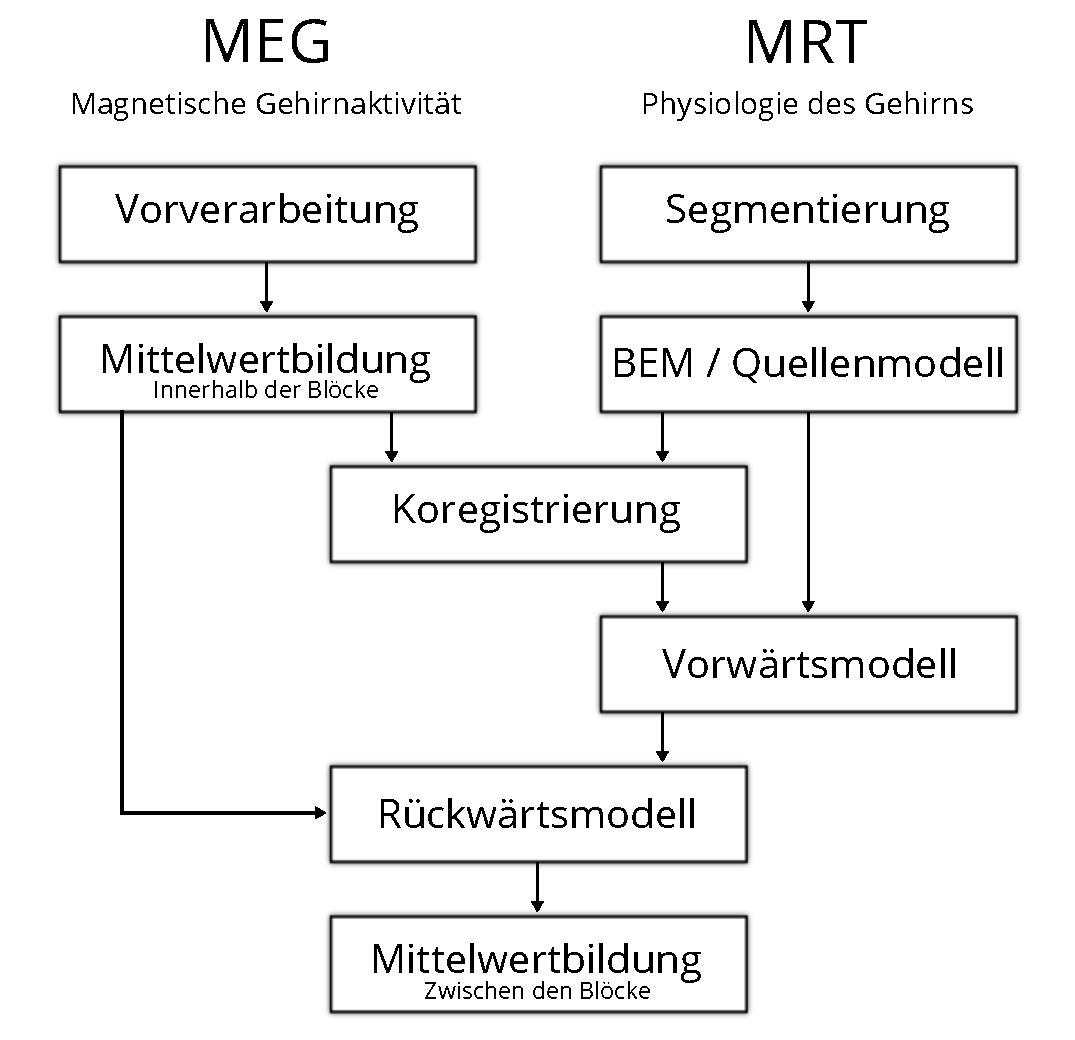
\includegraphics[width=0.65\textwidth]{methodik/verarbeitung.eps}}
  \vspace*{3mm}
  \caption[Schema der Datenverarbeitung]{Schema der Datenverarbeitung. Berechnet wurde dieses Verfahren für 2~Versuchspersonen in jeweils 6~Bedingungen.}
  \label{img:verfahren}
\end{figure}

Zusätzlich zum MEG-Datensatz mit den Aktivitätsdaten, wurde ein MRT-Datensatz verwendet, der einen einfachen Scan des Gehirns der Versuchspersonen enthielt. Für den MRT-Datensatz wurde zunächst eine Separation mittels \emph{Freesurfer} durchgeführt. Aus den Daten wurde ein Einschalen-BEM-Netz mit 10242 Punkten pro Hemisphäre berechnet. Im Einschalen-Modell werden nur solche Ströme vernachlässigt, die sich außerhalb des Schädels und im Schädelknochen selbst befinden. Für den Bereich innerhalb des Schädels wird die erwähnte anisotrope Leitfähigkeit angenommen. Dieses Modell ist eine starke Vereinfachung der realen Bedingungen, deren Eigenschaften jedoch ausreichend sind \parencite{stenroos2014comparison}.

Da nur Aktivität am Außenbereich von Interesse ist, wird und nicht im Inneren des Gehirns ist die Berechnung des BEM-Netzes in diesem Fall ausreichen. Am Rand des Gehirns wird überwiegend graue Substanz mit isotroper Leitfähigkeit erwartet (siehe auch Abschnitt \nameref{sec:segment} auf Seite \pageref{sec:segment}).

Die physiologischen Informationen des MRT-Datensatzes lagen in einem Koordinatensystem mit einer RAS-Orientierung vor (siehe auch Abschnitt~\nameref{sec:coreg} aus Seite~\pageref{sec:coreg}). Das Koordinatensystem wird anhand der Commissura anterior und der Commissura posterior definiert. Dabei liegt die $x$-$y$-Ebene so, dass die beiden Kommissuren geschnitten werden. Die z-Achse orientiert sich an der Fissura longitudinalis cerebri, also dem Interhemisphärenspalt. Das Koordinatensystem ist äquivalent zu Talairach und MNI (Montreal Neurological Institute). Die Einheiten liegen in Millimeter vor. Die Aktivitätsdaten des MEG wurden ebenfalls in einem RAS-orientierten Koordinatensystem gespeichert. Zur Aufstellung des Koordinatensystems werden an den zwei Ohren die präaurikularen Punkte bestimmt (Tragus) und die Nase (Nasion). Diese drei Punkte bilden die $x$-$y$-Ebene. Im Zentrum der drei Punkte wird die $z$-Achse definiert. Die Einheiten werden in Meter angegeben. Nach der Koregistrierung lag die Abweichung für \texttt{pa07} bei $1,3\,mm$, die Abweichung von \texttt{pa10} bei $2,2,mm$.

Jeder Durchgang (Trial) innerhalb der Blöcke, d.h. jedes Abspielen eines Tons und Aufzeichnen der Aktivitäten umfasste $500\,ms$. Die $100\,ms$ vor dem Abspiele eines Tons wurden als Baseline genutzt, es wurde die Spontanaktivität des Gehirns aufgezeichnet. Weitere $400\,ms$ wurden nach dem Abspielen des Tons als Signal-Anteil verwendet. Innerhalb dieser $400\,ms$ erfolgte das Auftreten der MMNm. Pro Block wurden $1370$ Trials verwendet, was $685\,s$ dauerte. Von denen waren $901$ Standards und $225$ Deviants. Die Gesamte Sequenz des Blockes wurde in seine Trials zerlegt, von denen die Deviants verwendet wurde.

Zusätzlich zur Auslese der gewünschten Trials, wurden alle Trials mit einem Hochpassfilter von $0,5\,Hz$ und einem Tiefpassfilter von $30\,Hz$ gefiltert. Um Trials in denen starke Störungen auftreten, wie heftige Augenbewegung oder starke Kopfbewegungen, zu verwerfen, wurde eine entsprechende Methode implementiert. In allen Daten sollten solche Signale gefunden werden, welche in den Magnetometern einen Ausschlag über $4\,pT$, in den Gradiometern über $200\,pT/m$ oder im EOG (Elektrookulografie, Erfassung der Augenbewegung) über $100\,\mu V$ aufwiesen. Sofern in einem Trial auch nur ein Datenpunkt mit einem höheren Wert auftrat, wurde der Trial verworfen. Eine Rauschunterdrückung mittels SSP, welche in FieldTrip enthalten ist, wurde deaktiviert.

Auf Grund der Annahme, dass die Versuchsperson ihren Kopf während eines Blocks nicht ändert, wurde bei den nicht-bewegungskorrigierten Daten (Rohdaten und SSS-Daten) die Aktivität innerhalb eines Blocks einfach gemittelt. Zwischen den Blöcken ist dies nicht möglich, wie im folgenden Abschnitt detailliert erläutert wird.

An dieser Stelle wurden die vorverarbeiteten Daten gespeichert und waren für die Quellrekonstruktion geeignet.

\subsection{Quellrekonstruktion}
\label{sec:lead-beam-mne}

Zur Berechnung des Vorwärtsmodells, d.h. die Wirkung der Quellen auf die Sensoren wird die Leadfield-Matrix verwendet, die in Abschnitt \nameref{sec:lead} auf Seite \pageref{sec:lead} eingeführt wurde. Die Liedfield-Matrix wird für eine bestimmte Kopfposition bestimmt. Die Signale die aus dem Gehirn kommen müssen von der gleichen Quelle aus immer auf die gleichen Sensoren abgebildet werden, andernfalls kommt es in der späteren Berechnung zu Fehlern. Wird eine falsche Kopfposition angenommen, werden gemessene Signale an den Sensoren später einer falschen bzw. verschobenen Quelle zugeordnet.

Innerhalb eines Blocks zwischen den Trials wird davon ausgegangen, dass sich die Versuchsperson bewegungslos verhält. Zwischen den Blöcken kommt es jedoch oft zu einer Unterbrechung der Messung und zu einem Neustart nach einer kurzen Pause. Eine deutliche Änderung der Kopfposition muss angenommen werden. Während bei SSS- und MC-Daten kein Problem auftritt, da hier die Kopfposition zwischen den Blöcken (SSS-Daten) bzw. sogar über die gesamten Daten (MC-Daten) korrigiert wird, ist dies bei den Rohdaten nicht der Fall. Eine Mittelung der Rohdaten über alle Blöcke hätte zur Folge, dass eigentlich vorhandene Aktivitäten verschwinden oder nicht vorhandene Aktivitäten auftauchen könnte. Würde die Leadfield-Matrix nur einmal beim ersten Block bestimmt werden, so wären die Rekonstruktionen in den drei weiteren Blöcken vermutlich stark fehlerbehaftet. Eine Mittelung der Trials über alle Blöcke kommt also zunächst nicht in Frage. Theoretisch gibt es zwei Möglichkeiten mit Rohdaten umzugehen:

Eine Möglichkeit ist die Korrektur der Kopfpositionen, ohne jedoch eine Rauschunterdrückung vorzunehmen. So bietet FieldTrip z.B. die Funktion \texttt{ft\_megrealign}. Die Korrektur der Kopfposition erfolgt durch eine Projektion der Sensordaten (z.B. der Rohdaten) auf eine grobe Quellrekonstruktion. Dazu wird unter Verwendung eines einfachen Kugelmodells als Vorwärtsmodell eine Lösung für ein unterbestimmtes inverses Problem geschätzt. Der Quellraum wird dabei ebenfalls vereinfacht als Kugeloberfläche angenommen. Durch Multiplikation der geschätzten Lösung mit der Leadfieldmatrix, welche die gewünschte Kopfpositin enthält, werden die korrigierten Daten erhalten. Bei diesem Verfahren kommt es wegen der enthaltenen vereinfachten Quellrekonstruktion zu Fehlern in den Daten, die Daten werden extrapoliert und enthalten nach der Korrektur nicht mehr die ursprünglichen Informationen. Es handelt sich nicht mehr um reine Rohdaten, weshalb dieses Verfahren nur einen Kompromiss darstellen würde.

Eine zweite Möglichkeit ist das Mitteln der rekonstruierten Quellaktivität. Für jeden Block kann eine eigene Leadfield-Matrix für das Vorwärtsmodell bestimmt werden. Nach anschließender Quelllokalisation können die Aktivitäten an den Quellen gemittelt werden (siehe auch Abbildung~\ref{img:verfahren}). Der Rechenaufwand ist zwar etwas erhöht, da für jeden Block die Leadfield-Matrix bestimmt werden muss, gleichzeitig bietet dieses Verfahren jedoch den Vorteil, dass es auch auf die rauschunterdrückten Daten von Maxfilter (SSS, MC) angewendet werden kann. Auch hier kann in der Vorverarbeitung absichtlich auf eine Mittelung über die Blöcke verzichtet werden. Die Leadfield-Matrizen können dann auch hier blockweise bestimmt und die Quellaktivitäten am Ende gemittelt werden. Diese Möglichkeit bietet damit eine optimale Vergleichbarkeit zwischen der Verwendung von Rodaten und rauschunterdrückten Daten, unabhängig vom verwendeten Lokalisationsverfahren.

Verwendet wurde auf Grund der besseren Vergleichbarkeit der Roh-, SSS- und MC-Daten die zweite Methode. Unabhängig vom Verfahren werden zunächst der Quellraum, der Volumenleiter und die vorverarbeiteten Aktivitätsdaten geladen. Wichtig ist, dass an dieser Stelle die Transformationsmatrix aus der Koregistrierung berücksichtigt wird, um die Koordinatensystem zu vereinen. Anschließend wird für jeden Block die Leadfield-Matrix berechnet. Abhängig von der Methode wird dann über \texttt{ft\_sourceanalysis} jeweils \texttt{beamformer\_lcmv} oder \texttt{minimumnormestimate} aufgerufen um die Quellen zu lokalisieren. Nach der Berechnung aller Blöcke für eine Versuchsperson für den jeweiligen Datensatz (Roh, SSS, MC) wurden die rekonstruierten Quellaktivitäten über alle Blöcke gemittelt und gespeichert. Die Auswertung der Daten erfolgte anschließend über die in Matlab enthaltene Funktion \texttt{plot} für die Zeitverläufe und die FieldTrip Methode \texttt{ft\_plot\_mesh} zur Darstellung der Aktivität.

Die gesamte Verarbeitung der Daten ist in Abbildung \ref{img:verfahren} in einem Schema dargestellt. Das abgebildete Verfahren wurde für die 2 Versuchspersonen in den jeweils 6 Bedingungen berechnet.

\subsection{Weitere Analysen}

Zur Auswertung der Daten wurden weitere Analysen durchgeführt. Die mit Hilfe der Kopfspulen zur Bestimmung der Kopfposition aufgezeichneten Daten wurden in einem Zeitverlauf dargestellt, um das Bewegungsverhalten der Versuchspersonen einschätzen zu können. Eine Frequenzanalyse der Versuchsperson \texttt{pa07} in Block 1 wurde für Roh- und SSS-Daten durchgeführt um das Rauschverhalten abschätzen zu können. Mit dem selben Zweck wurde das Signal-Rausch-Verhältnis für beide Versuchspersonen und alle Blöcke bestimmt.

%%% Hier evtl. noch Anpassungsgüte erwähnen? Sofern noch durchgeführt..

\subsection{Vergleichbarkeit der Lösungen}
\label{sec:amplitud}

Die Aktivität der Quellen aus den Rekonstruktionen von LCMV Beamformer und Minimum Norm Estimate unterscheiden sich. Die Stärke der Dipole (Stromdipolmomente) wird in~$Am$ angegeben. Dies wird von Minimum Norm Estimate als solches berechnet und kann auch als solches interpretiert werden. Bei Beamformer werden die Aktivitäten durch den räumlichen Filter bestimmt und sind Einheitenlos. Die Daten aus dem Beamformer-Verfahren müssen auf andere Weise interpretiert werden. Während bei Minimum Norm Estimate die Aktivität auf einer optimalen Gesamtlösung basiert und damit immer ein Kompromiss zwischen verschiedenen Aktivitäten gefunden werden muss, kann Beamformer für jeden einzelnen Dipol eine von anderen Quellaktivitäten unabhängige Aktivität ansetzen. Das führt dazu, dass vor allem im Zeitverlauf Amplituden auftreten können, die in ihrer Höhe über- oder unterschätzt werden können. Um eine vergleichbare Interpretation zu ermöglichen werden die Aktivitäten normiert. Aus den ersten $100\,ms$, der Baseline, wird ein Mittelwert gebildet, mit dem jede Aktivität im Zeitverlauf normiert wird.

Beiden Verfahren ist gemeinsam, dass die Lösung dreidimensional berechnet wird. Von Interesse ist aber lediglich der Betrag für jeden Ort. Um eine eindimensionale Lösung zu erhalten, wurde die Summe der Quadrate der drei Komponenten gebildet, welche im Quadrat der Amplitude resultiert.

% #######################
% ##### ERGEBNISSE  #####
% #######################

\newpage
\section{Ergebnisse}
\label{sec:ergebnisse}

Im Ergebnis zeigte sich, dass die Hypothese nicht bestätigt werden konnte. Im Gegenteil scheint LCMV Beamformer große Probleme mit der Auswertung von Rohdaten zu haben. Auch Minimum Norm Estimate hat Schwierigkeiten in der Auswertung von Rohdaten, zeigt im Vergleich jedoch bessere Ergebnisse. Unter Verwendung der gefilterten Daten (SSS und MC) zeigte Minimum Norm Estimate deutlich bessere Ergebnisse. Es werden im Folgenden zunächst einige Voranalysen betrachtet, bevor dann die eigentliche Quellrekonstruktion verglichen wird.

\subsection{Bewegungsprofile}
\label{sec:bewegung}

Bewegungen der Versuchspersonen sind als Störfaktoren zu bewerten. Je mehr sich eine Versuchsperson bewegt, desto schlechter werden die Lösungen ausfallen. Um die Bewegung der Versuchspersonen abschätzen zu können, werden zusätzliche aktive Spulen am Kopf der Versuchsperson angebracht. Die Bewegungen können mit Hilfe der MEG-Sensoren erfasst werden. Bei der Korrektur der Daten mittels MC von MaxFilter werden diese Daten ausgewertet und können mittels eines einfachen Matlab-Skripts verarbeitet werden. In den Abbildungen \ref{img:bewegung} sind die Bewegungsprofile der beiden Versuchspersonen für alle Blöcke dargestellt. Während die Bewegungen von Versuchsperson \texttt{pa07} über die Blöcke hinweg im Bereich von ca. $2$-$4\,mm$ liegen, bewegt sich Versuchsperson \texttt{pa10} im Bereich von ca. $4$-$6\,mm$. Bei MEG-Messungen sind Bewegungen von mehr als $5\,mm$ nicht ungewöhnlich \parencite{wilson2007continuous}. Beide Versuchspersonen liegen also im Rahmen gewöhnlicher Messungen.

\begin{figure}
%  \centering
  \captionsetup{justification=centering}
  %
  \begin{subfigure}[c]{0.23\textwidth}
    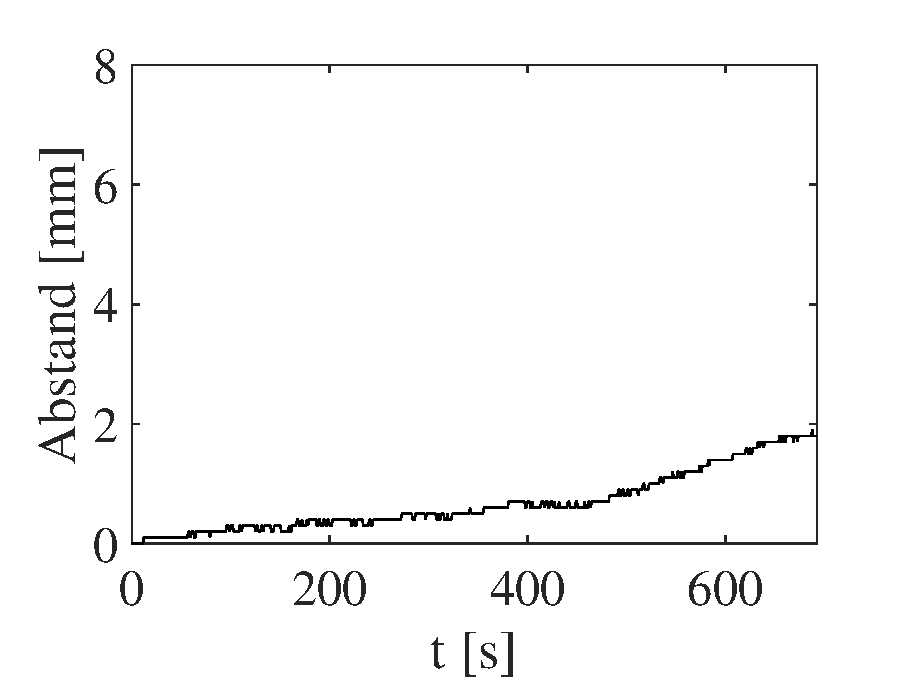
\includegraphics[width=\textwidth]{ergebnisse/movement/pa07a1_mc_dist_movement.eps}
    \subcaption{VP \texttt{pa07}, Block 1}
    \label{img:bewegung:pa07:1}
  \end{subfigure}\hspace*{0.02\textwidth}
  %
  \begin{subfigure}[c]{0.23\textwidth}
    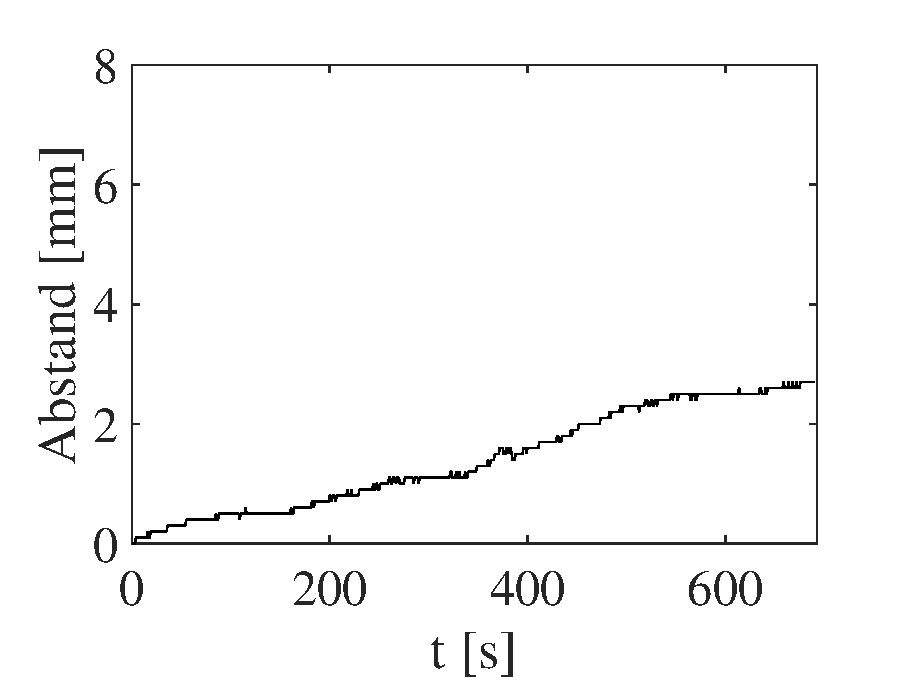
\includegraphics[width=\textwidth]{ergebnisse/movement/pa07a3_mc_dist_movement.eps}
    \subcaption{VP \texttt{pa07}, Block 3}
    \label{img:bewegung:pa07:3}
  \end{subfigure}\hspace*{0.02\textwidth}
  %
  \begin{subfigure}[c]{0.23\textwidth}
    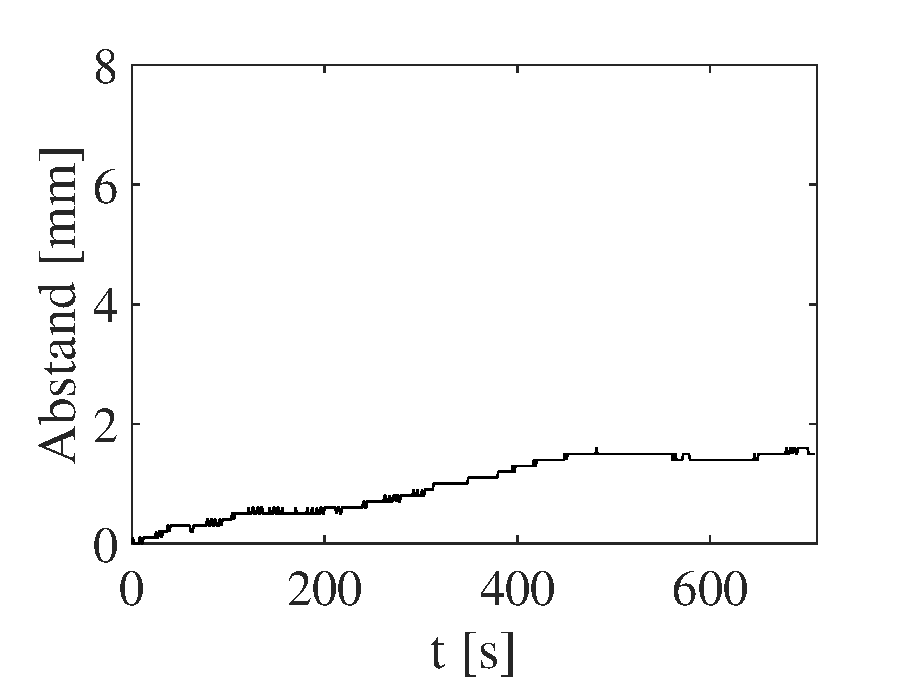
\includegraphics[width=\textwidth]{ergebnisse/movement/pa07a4_mc_dist_movement.eps}
    \subcaption{VP \texttt{pa07}, Block 4}
    \label{img:bewegung:pa07:4}
  \end{subfigure}\hspace*{0.02\textwidth}
  %
  \begin{subfigure}[c]{0.23\textwidth}
    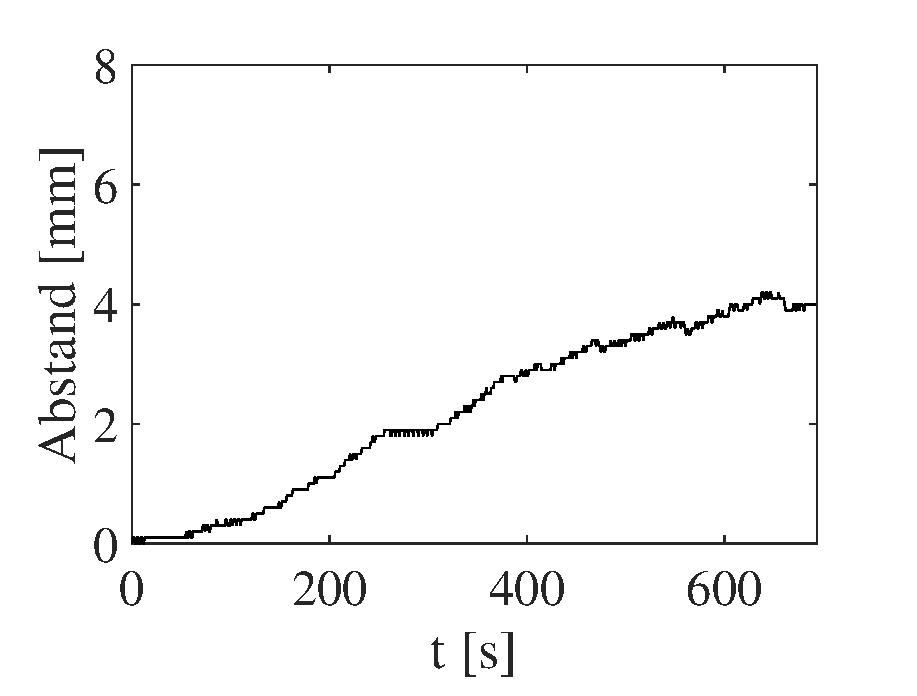
\includegraphics[width=\textwidth]{ergebnisse/movement/pa07a6_mc_dist_movement.eps}
    \subcaption{VP \texttt{pa07}, Block 6}
    \label{img:bewegung:pa07:6}
  \end{subfigure}\vspace*{0.04\textwidth}
  %
  \begin{subfigure}[c]{0.23\textwidth}
    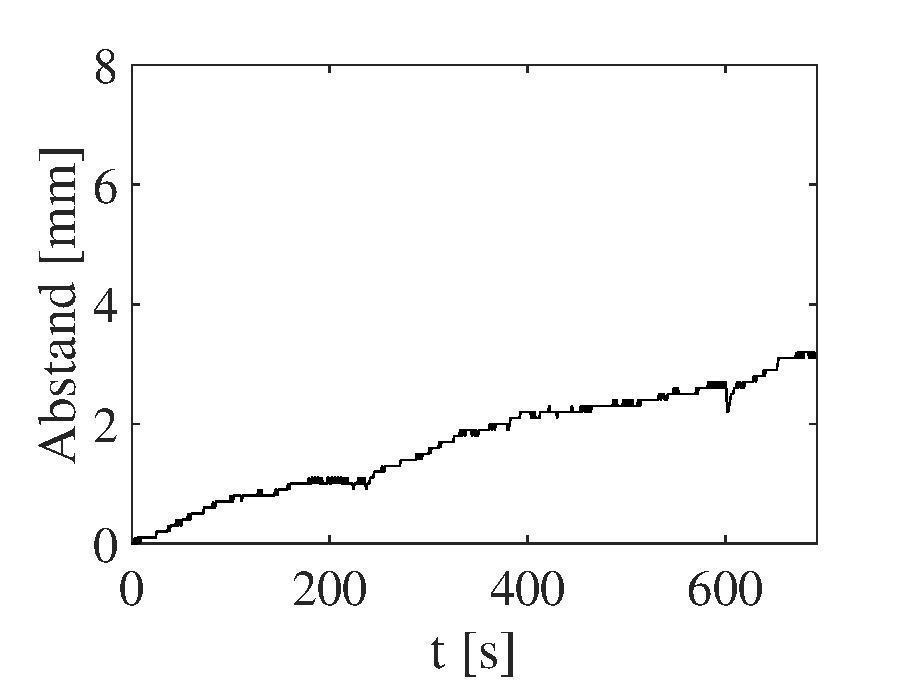
\includegraphics[width=\textwidth]{ergebnisse/movement/pa10a1_mc_dist_movement.eps}
    \subcaption{VP \texttt{pa10}, Block 1}
    \label{img:bewegung:pa10:1}
  \end{subfigure}\hspace*{0.02\textwidth}
  %
  \begin{subfigure}[c]{0.23\textwidth}
    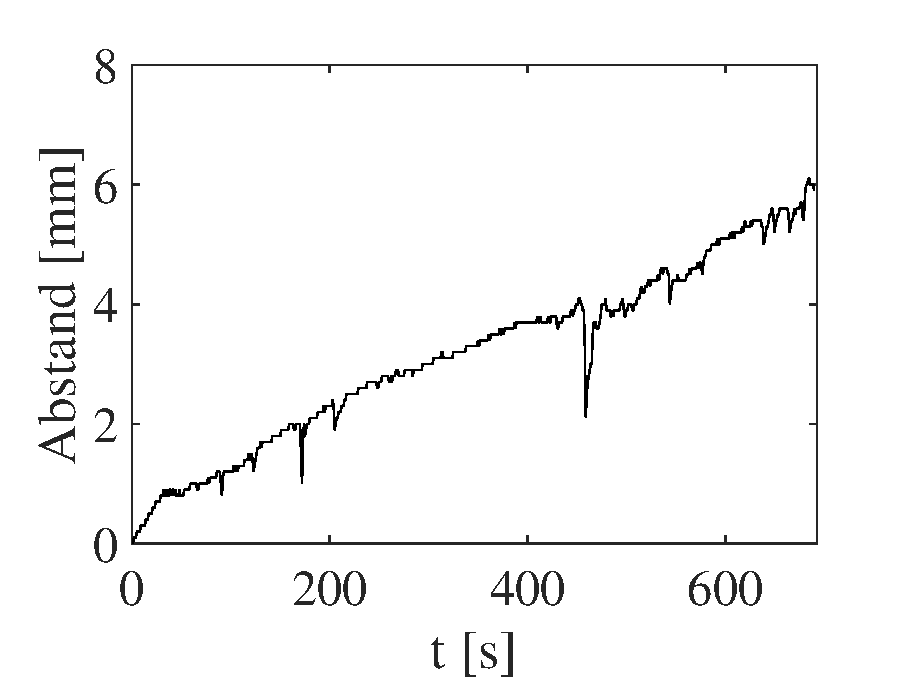
\includegraphics[width=\textwidth]{ergebnisse/movement/pa10a3_mc_dist_movement.eps}
    \subcaption{VP \texttt{pa10}, Block 3}
    \label{img:bewegung:pa10:3}
  \end{subfigure}\hspace*{0.02\textwidth}
  %
  \begin{subfigure}[c]{0.23\textwidth}
    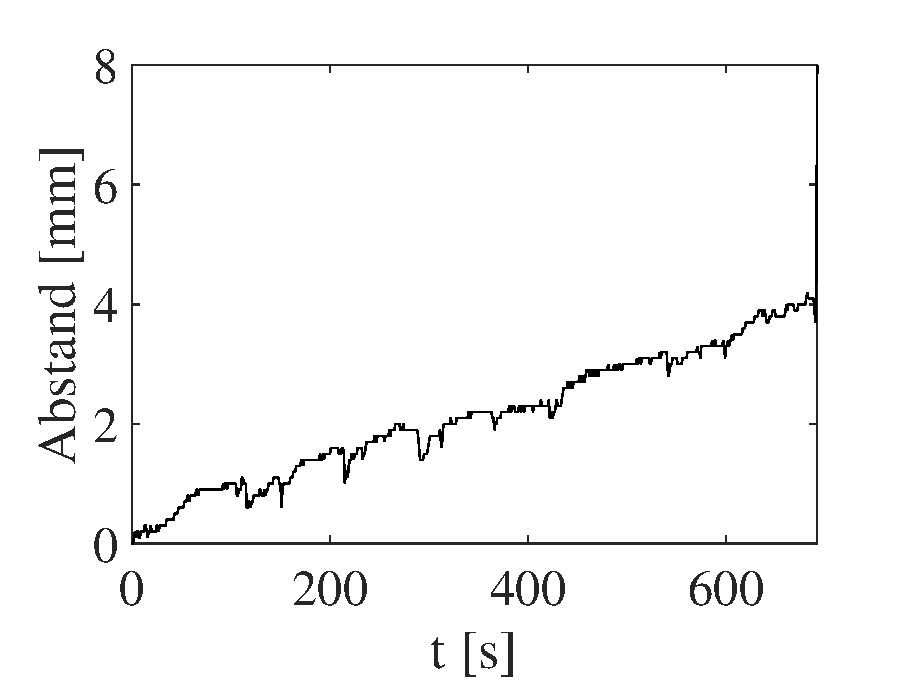
\includegraphics[width=\textwidth]{ergebnisse/movement/pa10a4_mc_dist_movement.eps}
    \subcaption{VP \texttt{pa10}, Block 4}
    \label{img:bewegung:pa10:4}
  \end{subfigure}\hspace*{0.02\textwidth}
  %
  \begin{subfigure}[c]{0.23\textwidth}
    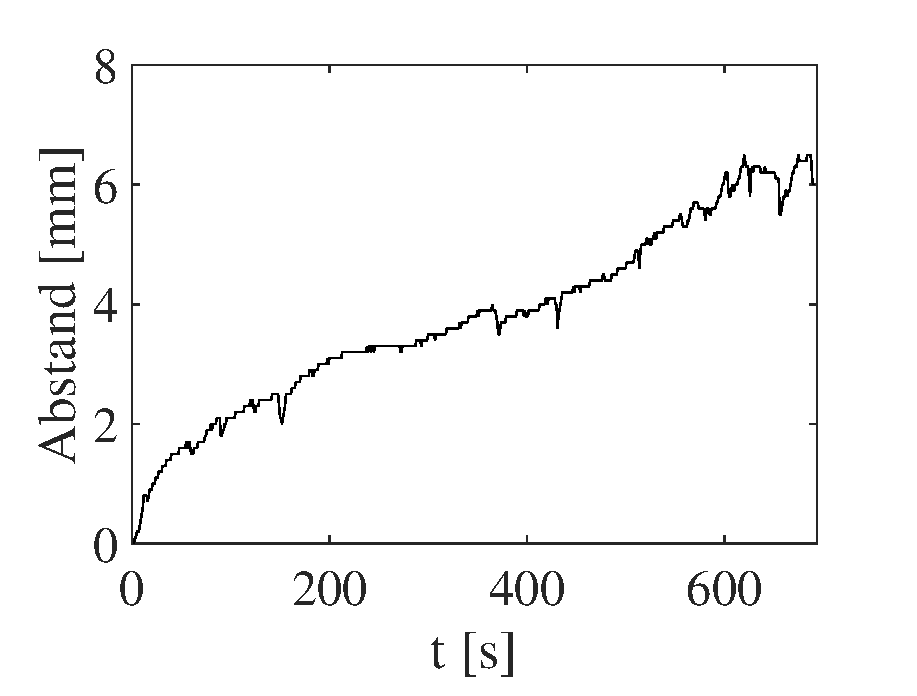
\includegraphics[width=\textwidth]{ergebnisse/movement/pa10a6_mc_dist_movement.eps}
    \subcaption{VP \texttt{pa10}, Block 6}
    \label{img:bewegung:pa10:6}
  \end{subfigure}
  %
  \captionsetup{justification=justified}
  \vspace*{3mm}
  \caption[Bewegungsprofile der Versuchspersonen]{Bewegungsprofile der Versuchspersonen in allen 4 Blöcken.}
  \label{img:bewegung}
\end{figure}

\subsection{Frequenzanalyse}
\label{sec:freq-analy}

Die Frequenzanalyse wurde nur für Versuchsperson \texttt{pa07} in Block 1 durchgeführt. Das Rauschverhalten sollte für alle Versuchspersonen in allen Blöcken sehr ähnlich sein. In Abbildung \ref{img:freq-analy} ist das Ergebnis dargestellt. In der Grafik \ref{img:freq-analy-raw} ist die Leistungsdichtespektrum auf Basis der Rohdaten, in Grafik \ref{img:freq-analy-sss} auf Basis der SSS-Daten dargestellt. Gezeigt wird exemplarisch die Analyse für die Kanäle \texttt{MEG1511}, \texttt{MEG2611}, \texttt{MEG1011} und \texttt{MEG2111} (siehe auch Abbildung~\ref{img:sensmap}). Während in den Rohdaten noch deutlich identifizierbare Artefakte enthalten sind, wie beispielsweise der Netzstrom mit $50\,Hz$ oder die Bahn-Oberleitung und deren Oberschwingungen bei $16,67\,Hz$, $33,33\,Hz$, etc., sind diese in den SSS-Daten nicht mehr oder deutlich vermindert. Die äußeren Quellen wurden herausgefiltert. Generell verläuft die rechte Frequenzanalyse deutlich glätter, als die auf den Rohdaten basierende. Damit wird deutlich welche Herausforderung die Lokalisationverfahren zu leisten haben um adäquate Ergebnisse hervorzubringen.

\begin{figure}
  \centering
  \captionsetup{justification=centering}
  %
  \begin{subfigure}[c]{0.47\textwidth}
    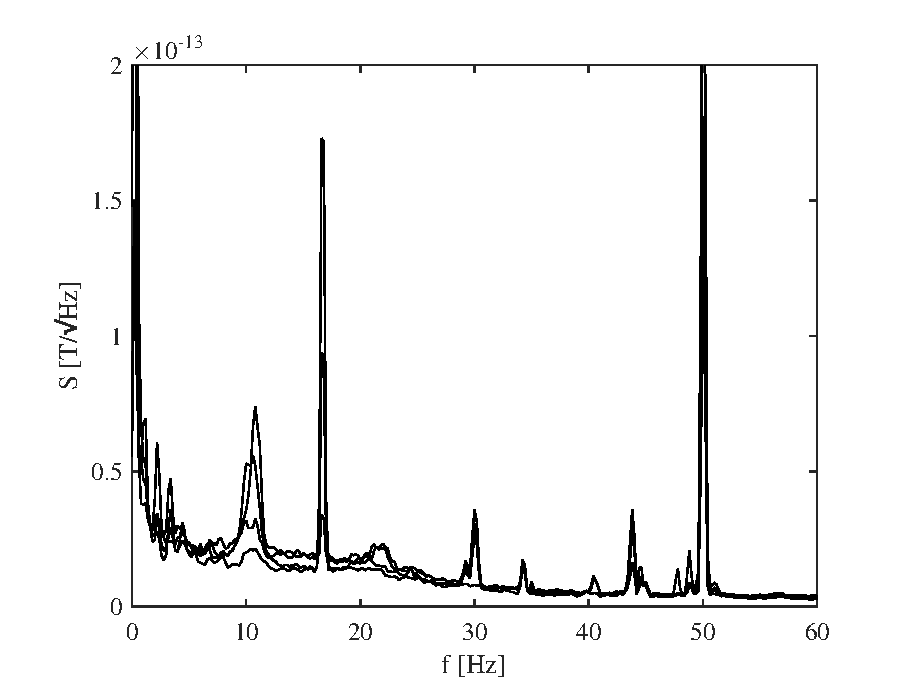
\includegraphics[width=\textwidth]{ergebnisse/pa07a1_raw_freq.eps}
    \subcaption{Leistungsdichtespektrum der Rohdaten}
    \label{img:freq-analy-raw}
  \end{subfigure}\hspace*{0.04\textwidth}
  %
  \begin{subfigure}[c]{0.47\textwidth}
    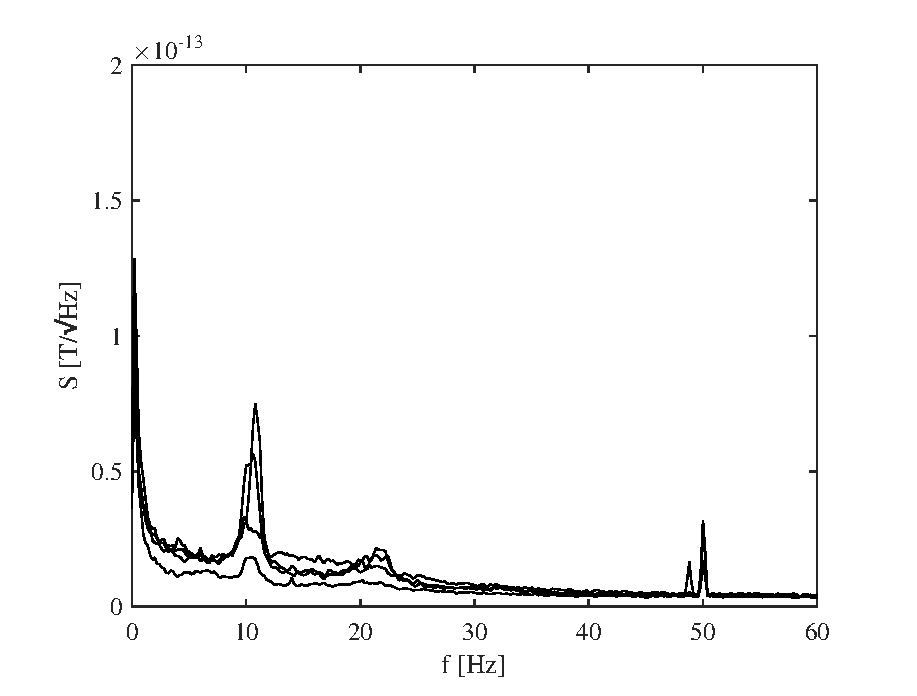
\includegraphics[width=\textwidth]{ergebnisse/pa07a1_sss_freq.eps}
    \subcaption{Leistungsdichtespektrum der SSS-Daten}
    \label{img:freq-analy-sss}
  \end{subfigure}
  %
  \captionsetup{justification=justified}
  \vspace*{3mm}
  \caption[Leistungsdichtespektrum auf Basis eines Blocks]{Leistungsdichtespektrum auf Basis der Daten von Versuchsperson~\texttt{pa07} von Block~1 für die Kanäle \texttt{MEG1511}, \texttt{MEG2611}, \texttt{MEG1011} und \texttt{MEG2111}. Deutlich wird die Abnahme des Rauschens durch die SSS-Filterung. Vor allem bei $50\,Hz$ (Netzstrom), $16,67\,Hz$ (Bahn-Oberleitung) und deren Oberschwingungen ist eine Abnahme der Amplitude offensichtlich. Eine Abnahme des Rauschens ist aber bspw. auch im Bereich $0\,Hz$ bis $5\,Hz$ sehr effektiv.}
  \label{img:freq-analy}
\end{figure}

\subsection{Signal-Rausch-Verhältnis}
\label{sec:snr}

Das Signal-Rausch-Verhältnis (signal-noise-ration, SNR) gibt das Amplitudenverhältnis der Daten an. Die Daten werden dabei in einen Rausch-Anteil $P_R$ und einen Signal-Anteil $P_S$ zerlegt. Allgemein gilt:

\begin{equation}
SNR = \frac{P_S}{P_R}
\end{equation}

Als Rausch-Anteil wurden die ersten 100 ms gewählt. Dies entspricht der Baseline. Als Signal-Anteil wurde die MMNm verwendet, welche im Bereich 150 ms bis 250 ms liegt (siehe auch Abbildungen~\ref{img:butterfly:grad} und~\ref{img:butterfly:mag}).

Es wurden nur jene Kanäle für die Berechnung verwendet, welche am Ort der Entstehung der MMNm entsprechende Signale messen. Dafür wurde zunächst das Amplitudenmaximum aus allen Trials und Zeitpunkten bestimmt. Für die zwei berechneten Versuchspersonen ergaben sich das Maximum an Kanal \texttt{MEG014} für \texttt{pa10} und Kanal \texttt{MEG151} für \texttt{pa07}. Das leicht verschobene Maximum ist auf eine unterschiedliche Position des Kopfes der Versuchsperson im MEG-Helm während des Versuchs zurück zu führen. Nachdem die Maxima bestimmt wurden, wurden die umliegenden Kanäle in die Berechnung des Signals integriert. Die verwendeten Kanäle sind:

\texttt{MEG013}, \texttt{MEG014}, \texttt{MEG021}, \texttt{MEG024}, \texttt{MEG151}, \texttt{MEG154}, \texttt{MEG152}, \texttt{MEG161}

In der Sensor-Karte in Abbildung~\ref{img:sensmap} wird deutlich, dass die Kanäle wie zu erwarten für die MMN im temporalen Bereich liegen. Von den Kanälen wurden sowohl die Magnetometer, als auch die beiden Gradiometer berücksichtigt.

Zur Berechnung des SNR wurden die Rohdaten verwendet, was eine erneute Vorverarbeitung nötig macht. Dabei wurde der gesamte Datensatz nach obigen Kriterien in die Trials zerteilt. Jeder Trail wurde anschließend in einen Rausch- und einen Signal-Anteil getrennt. Von der Baseline (Rausch-Anteil) wurde der Mittelwert gebildet.

\begin{equation}
\bar{b}_{ik} = \frac{1}{n_b} \sum_{j=1}^{n_b} b_{ijk}
\end{equation}

Dabei ist $i$ der Index der Kanäle, $j$ der Index der Zeitpunkte und $k$ der Index der Trials. $n_b$ entspricht der Anzahl der Zeitpunkt, die innerhalb der Baseline berücksichtigt werden mit $n_b = 100$. $b_{ijk}$ entspricht einer dreidimensionalen Datenstruktur, welche die Amplituden für alle Trials, Zeitpunkt und Kanäle enthält. Gemittelt über die Zeitpunkt ergibt sich eine zweidimensionale Matrix $b_{ik}$, welche eine mittlere Amplitude für jeden Trial und jeden Kanal enthält.

\begin{figure}
  \centering
%  \captionsetup{justification=centering}
  %
  \setlength{\fboxsep}{5mm}
  \fbox{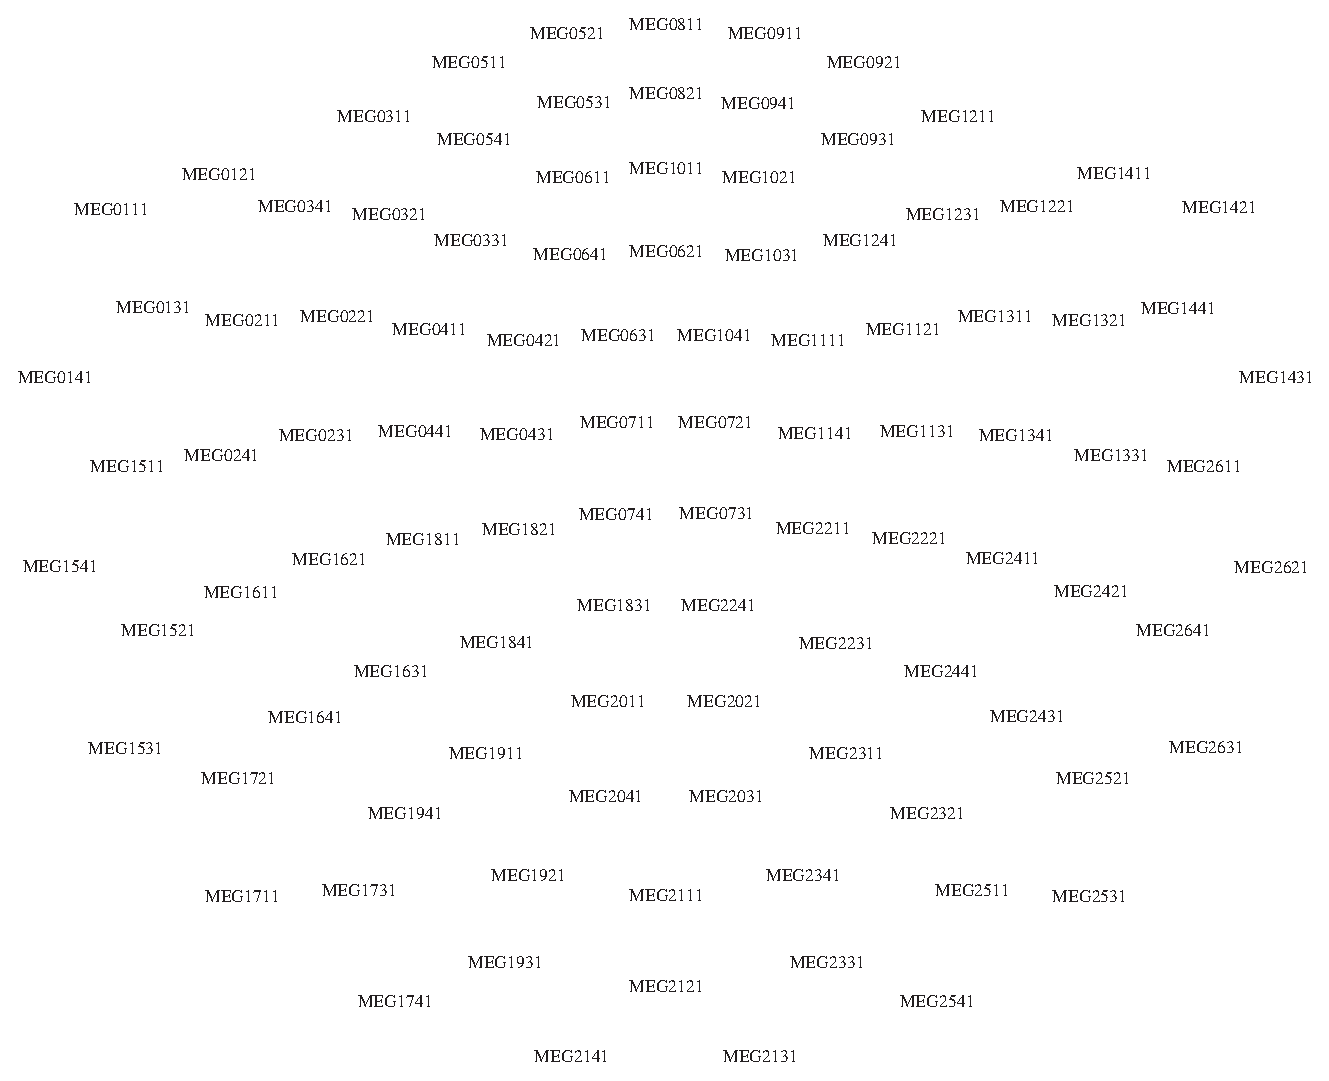
\includegraphics[width=0.92\textwidth]{ergebnisse/sensormap.eps}}
  \vspace*{3mm}
  \caption[Karte der Sensoren des \emph{Vectorview} MEG-Gerätes]{Karte der Sensoren des \emph{Vectorview} MEG-Gerätes in zweidimensionaler Darstellung. Dargestellt sind die Bezeichnungen der Magnetometer. Im oberen Bereich liegt die Stirn, im unteren Bereich der Hinterkopf der Versuchsperson.}
  \label{img:sensmap}
\end{figure}

Dieser Mittelwert wird für jeden einzelnen Zeitpunkt innerhalb der gesamten Aktivität (sowohl für den Rausch-Anteil, als auch für den Signal-Anteil) subtrahiert, um das mittlere Rauschen aus der Aktivität heraus zu rechnen.

\begin{equation}
\hat{b}_{im} = b_{im} - \bar{b}_{ik} \quad \text{und} \quad \hat{s}_{im} = s_{im} - \bar{b}_{ik}
\end{equation}

Dabei wurden die Zeitpunkte~$j$ und die Trials~$k$ zusammengefasst im Index~$m$, eine Trennung dieser beiden Indizes ist an der Stelle nicht mehr notwendig, es handelt sich nur noch um eine Anzahl von Trials~$m$. $\hat{b}_{im}$~entspricht dem korrigierten Rausch-Anteil und $\hat{s}_{im}$~dem korrigierte Signal-Anteil.

Die neuen Matrizen werden anschließend durch die Anzahl der Zeitpunkt geteilt. Dieser formale Schritt ist nötig für den Fall, dass sich die Zeitbereiche der beiden Anteile unterscheiden. In diesem Fall liegen beide bei $n_b = n_s = 100$ Zeitpunkten, so dass dieser Schritt auch ausgelassen werden könnte. Der Vollständigkeit halber:

\begin{equation}
\tilde{b}_{im} = \frac{\hat{b}_{im}}{n_b} \quad \text{und} \quad \tilde{s}_{im} = \frac{\hat{s}_{im}}{n_s}
\end{equation}

\begin{table}[t]
  \caption{}
  \label{tab:snr}
  \vspace*{3mm}
  \centering
  \setlength{\tabcolsep}{1cm}
  \renewcommand{\arraystretch}{1.5}
  \begin{tabular}{ccc}
  \hline
  Block & pa07 & pa10 \\
  \hline
  1 & $3.123$ & $3.915$\\
  3 & $2.942$ & $3.144$\\
  4 & $2.589$ & $3.875$\\
  6 & $2.715$ & $3.348$\\
  \hline
  \end{tabular}
  \vspace*{3mm}
  \caption*{Signal-Rausch-Verhältnis für zwei Versuchspersonen in jeweils 4 Blöcken. Das Verhältnis sollte im Idealfall einen Wert von $3$ überschreiten.}
\end{table}

Im folgenden Schritt werden die Kovarianzen für die beiden Anteile bestimmt.

\begin{equation}
b_{ij} = \tilde{b}_{im} \cdot \tilde{b}_{mj} \quad \text{und} \quad s_{ij} = \tilde{s}_{im} \cdot \tilde{s}_{mj}
\end{equation}

$b_{mj}$ bzw. $s_{mj}$ entspricht dabei der transponierten Matrix von~$b_{im}$ bzw.~$s_{im}$, wobei~$i$ und~$j$ jeweils den Index des Kanals bezeichnet. Die Varianzmatrizen mit den Einträgen~$b_{ij}$ und~$s_{ij}$ sind quadratisch und enthalten die Kovarianzen der Amplituden zwischen allen Kanälen. Die Diagonalelemente der Matrizen entsprechen dann den Varianzen der Kanäle. Die Varianzen werden komponentenweise dividiert und summiert:

\begin{equation}
SNR = \sum_i \delta_{ij} \frac{s_{ij}}{b_{ij}}
\end{equation}

Die SNR sollte im Idealfall oberhalb von~$3$ liegen. Dieser Wert ist willkürlich, wird jedoch von der Software \emph{MNE} als Standardwert verwendet und soll in diesem Zusammenhang als Orientierung dienen, da die Software für entsprechende Berechnungen üblicherweise eingesetzt wird. Die Ergebnisse sind in Tabelle \ref{tab:snr} dargestellt. Deutlich wird, dass das Signal-Rausch-Verhältnis um den Wert von $3$ liegt. Während \texttt{pa07} eher leicht unterhalb von $3$ liegt, sind die Werte von \texttt{pa10} gut oberhalb von $3$. Das Signal-Rausch-Verhältnis spricht dafür, dass die Daten zur Lokalisation geeignet sein sollten.

\subsection{Vorverarbeitung}
\label{sec:ergebnis-vorverarbeitung}

\begin{table}
  \caption{}
  \label{tab:rejecting}
  \vspace*{3mm}
  \centering
  \setlength{\tabcolsep}{7mm}
  \renewcommand{\arraystretch}{1.5}
  \begin{tabular}{ccccccc}
  \hline
  & \multicolumn{3}{c}{pa07} & \multicolumn{3}{c}{pa10}\\
  Block & Roh & SSS & MC & Roh & SSS & MC \\
  \hline
  1 & $193$ & $198$ & $198$ & $155$ & $155$ & $155$\\
  3 & $192$ & $209$ & $208$ & $143$ & $145$ & $145$\\
  4 & $57$ & $198$ & $195$ & $157$ & $158$ & $158$\\
  6 & $163$ & $177$ & $175$ & $145$ & $145$ & $145$\\
  \hline
  \end{tabular}
  \vspace*{3mm}
  \caption*{Verwendete Trials innerhalb jeden Blocks für beide Versuchspersonen und alle verwendeten Daten. Es standen pro Block 225 Deviant-Trials zur Verfügung.}
\end{table}

In der Vorverarbeitung wurden bereits Trials mit hohen Abweichungen herausgefiltert. Dies führte dazu, dass mehr Trials innerhalb der Rohdaten herausgefiltert wurden, da hier die Amplituden häufiger die Grenzwerte überschritten. In Tabelle \ref{tab:rejecting} sind die Anzahl der verwendeten Trials pro Block, Datenquelle und Versuchsperson aufgeführt. Leichte Verbesserungen ermöglicht das SSS-Verfahren, vor allem bei \texttt{pa07}. Sehr auffällig ist der Wert von \texttt{pa07} im vierten Block bei den Rohdaten. Welche genauen Bedingungen zu diesem Ergebnis geführt haben sind nicht bekannt. In Abbildung \ref{img:butterfly:pa07:4:raw} ist die Aktivität Magnetometer dargestellt. Deutlich wird, dass hier starke Störungen vorliegen, vor allem im Vergleich der Rohdaten anderer Blöcke (siehe Abbildungen~\ref{img:butterfly:grad} und~\ref{img:butterfly:mag}). Erstaunlich ist jedoch, dass SSS diese Störung nahezu vollständig eliminieren kann. Die Ursache der Störung liegt also mit hoher Wahrscheinlichkeit außerhalb des MEG-Helms. Die SSS-Korrigierten Daten der Magnetometer sind in Abbild \ref{img:butterfly:pa07:4:sss} im Vergleich dargestellt.

Die Annahme, dass bei Versuchsperson~\texttt{pa10} ein erheblich größerer Unterschied zwischen SSS-Daten und MC-Daten vorliegen müsste, als bei \texttt{pa07}, da sich Versuchsperson~\texttt{pa10} mehr bewegt hat, scheint nicht zuzutreffen. Die Bewegung von \texttt{pa10} scheint keinen großen Einfluss zu haben. 

%%% Referenz zu anderen Butterfly-Diagrammen!

\begin{figure}
%  \centering
  \captionsetup{justification=centering}
  %
  \begin{subfigure}[c]{0.47\textwidth}
    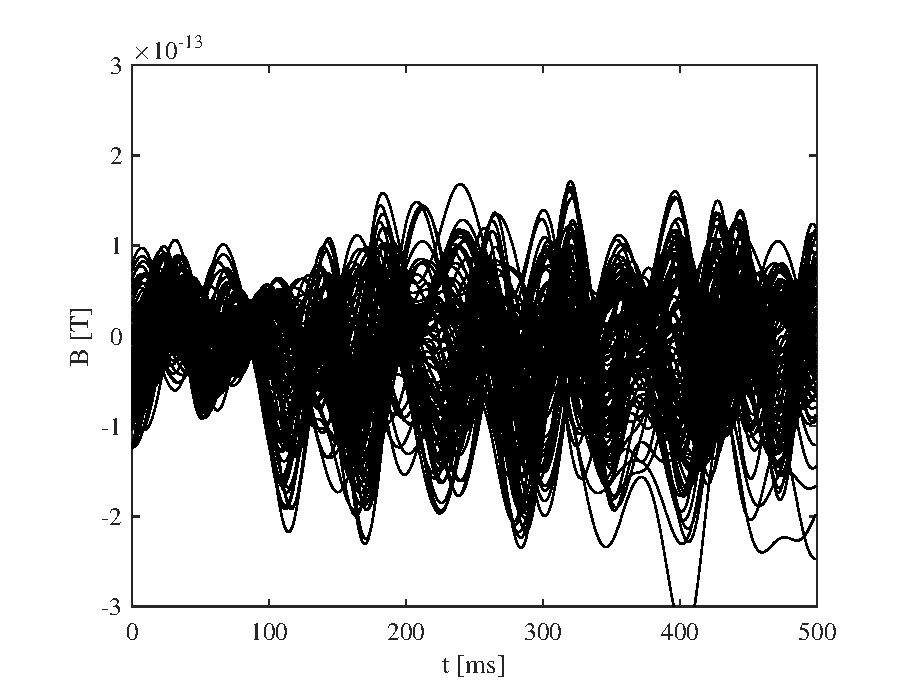
\includegraphics[width=\textwidth]{ergebnisse/butterfly/pa07a4_eve2_raw_mag_butterfly.eps}
    \subcaption{Rohdaten}
    \label{img:butterfly:pa07:4:raw}
  \end{subfigure}\hspace*{0.04\textwidth}
  %
  \begin{subfigure}[c]{0.47\textwidth}
    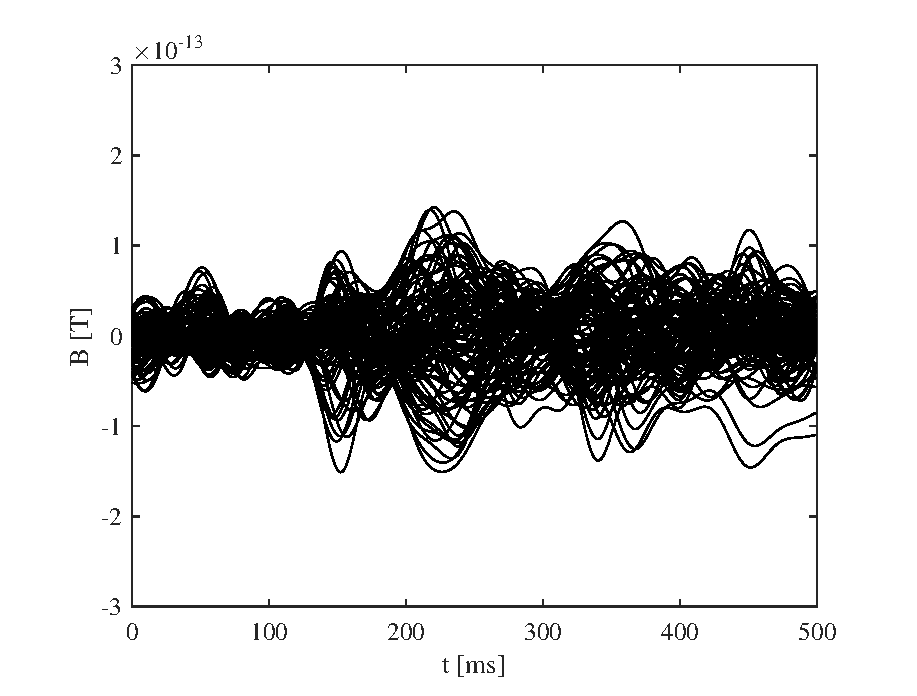
\includegraphics[width=\textwidth]{ergebnisse/butterfly/pa07a4_eve2_sss_mag_butterfly.eps}
    \subcaption{SSS-korrigierte Daten}
    \label{img:butterfly:pa07:4:sss}
  \end{subfigure}
  %
  \captionsetup{justification=justified}
  \vspace*{3mm}
  \caption{Kanalaktivität der Magnetometer der Rohdaten und der SSS-korrigierten Daten in Block 4 von Versuchsperson \texttt{pa07}.}
  \label{img:butterfly:pa07:4}
\end{figure}

\begin{figure}
  \centering
  \captionsetup{justification=centering}
  %
  \begin{subfigure}[c]{0.36\textwidth}
    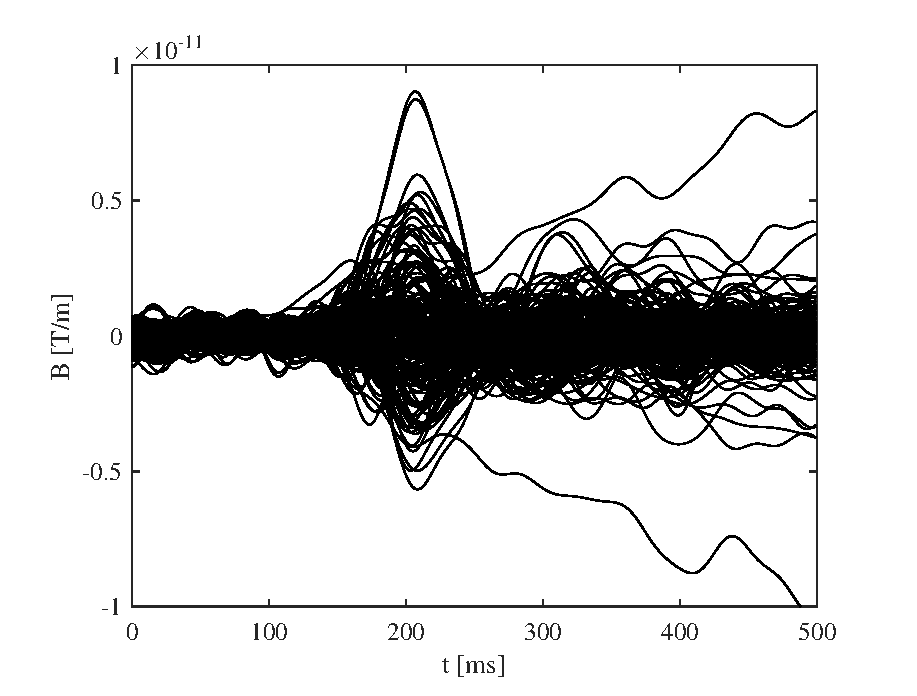
\includegraphics[width=\textwidth]{ergebnisse/butterfly/pa07a1_eve2_raw_grad_butterfly.eps}
    \subcaption{VP \texttt{pa07}, Rohdaten}
    \label{img:butterfly:grad:raw:pa07}
  \end{subfigure}\hspace*{0.08\textwidth}
  %
  \begin{subfigure}[c]{0.36\textwidth}
    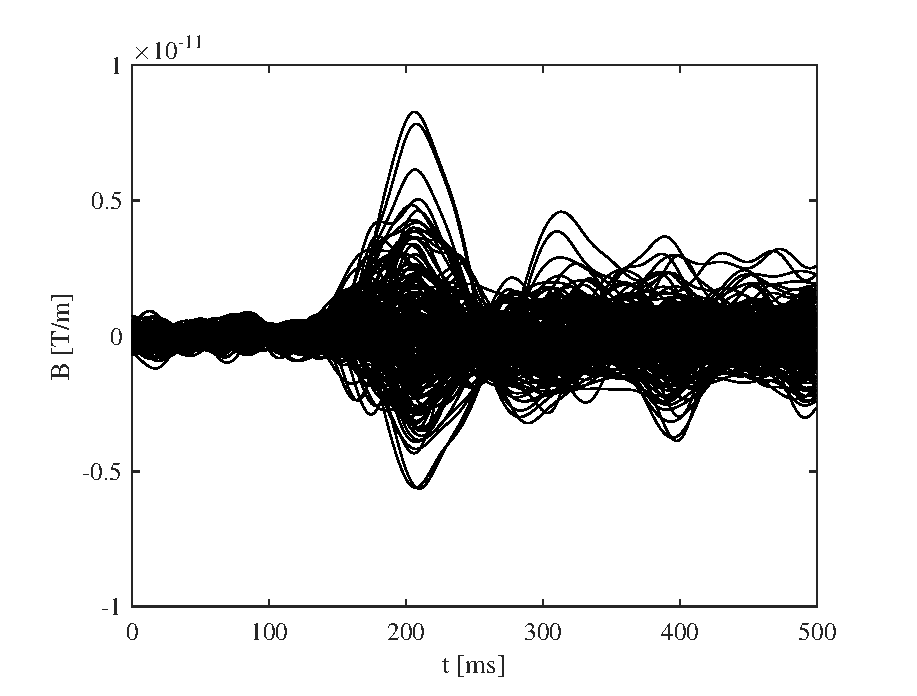
\includegraphics[width=\textwidth]{ergebnisse/butterfly/pa07a1_eve2_sss_grad_butterfly.eps}
    \subcaption{VP \texttt{pa07}, SSS-Daten}
    \label{img:butterfly:grad:sss:pa07}
  \end{subfigure}\vspace*{0.02\textwidth}
  %  
  \begin{subfigure}[c]{0.36\textwidth}
    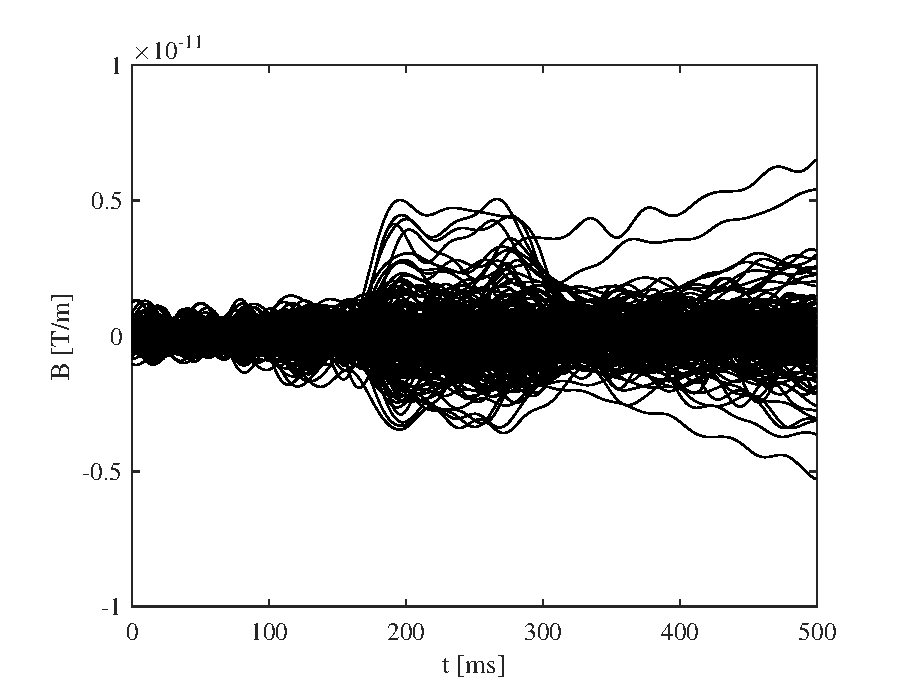
\includegraphics[width=\textwidth]{ergebnisse/butterfly/pa10a1_eve2_raw_grad_butterfly.eps}
    \subcaption{VP \texttt{pa10}, Rohdaten}
    \label{img:butterfly:grad:raw:pa10}
  \end{subfigure}\hspace*{0.08\textwidth}
  %
  \begin{subfigure}[c]{0.36\textwidth}
    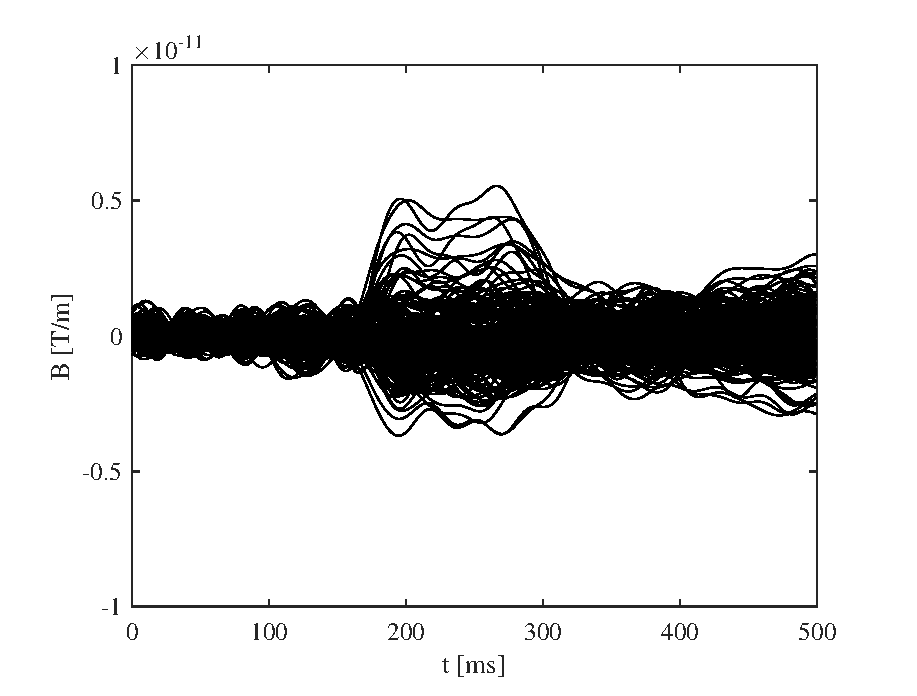
\includegraphics[width=\textwidth]{ergebnisse/butterfly/pa10a1_eve2_sss_grad_butterfly.eps}
    \subcaption{VP \texttt{pa10}, SSS-Daten}
    \label{img:butterfly:grad:sss:pa10}
  \end{subfigure}
  %
  \captionsetup{justification=justified}
  \vspace*{3mm}
  \caption[Gemessene Aktivität an den Gradiometern]{Gemessene Aktivität an den Gradiometern für beide Versuchspersonen, jeweils in Block 1 mit Rohdaten und SSS-Daten.}
  \label{img:butterfly:grad}
  %
  \vspace*{5mm}
  %
  \centering
  \captionsetup{justification=centering}
  \begin{subfigure}[c]{0.36\textwidth}
    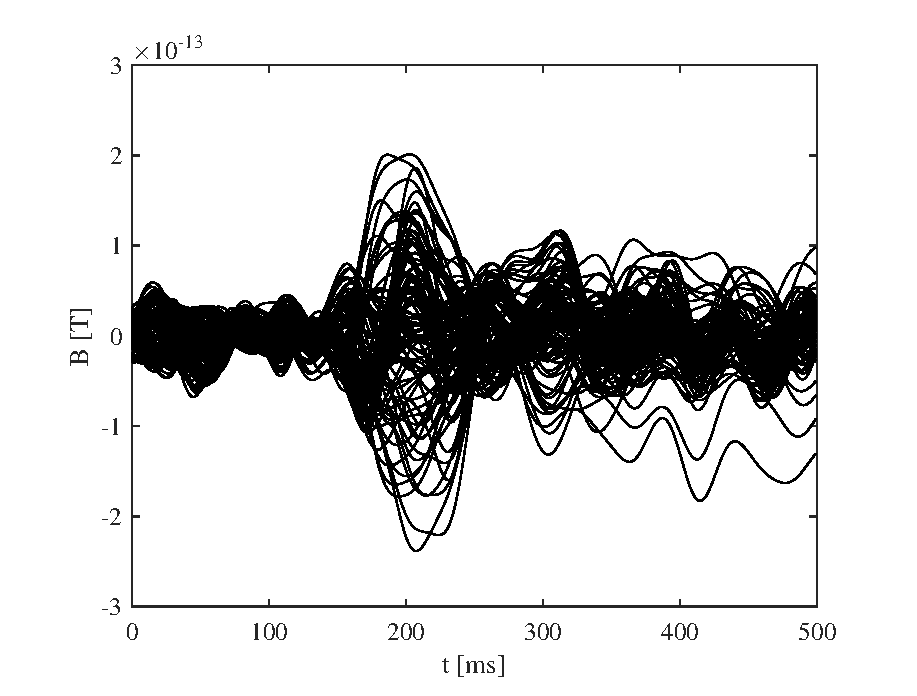
\includegraphics[width=\textwidth]{ergebnisse/butterfly/pa07a1_eve2_raw_mag_butterfly.eps}
    \subcaption{VP \texttt{pa07}, Rohdaten}
    \label{img:butterfly:mag:raw:pa07}
  \end{subfigure}\hspace*{0.08\textwidth}
  %
  \begin{subfigure}[c]{0.36\textwidth}
    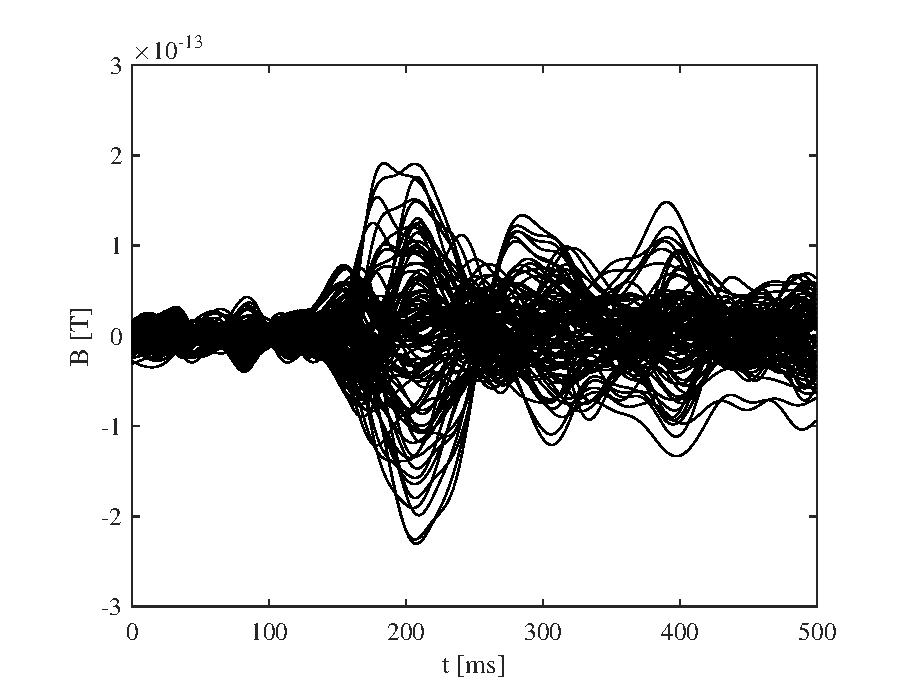
\includegraphics[width=\textwidth]{ergebnisse/butterfly/pa07a1_eve2_sss_mag_butterfly.eps}
    \subcaption{VP \texttt{pa07}, SSS-Daten}
    \label{img:butterfly:mag:sss:pa07}
  \end{subfigure}\vspace*{0.02\textwidth}
  %
  \begin{subfigure}[c]{0.36\textwidth}
    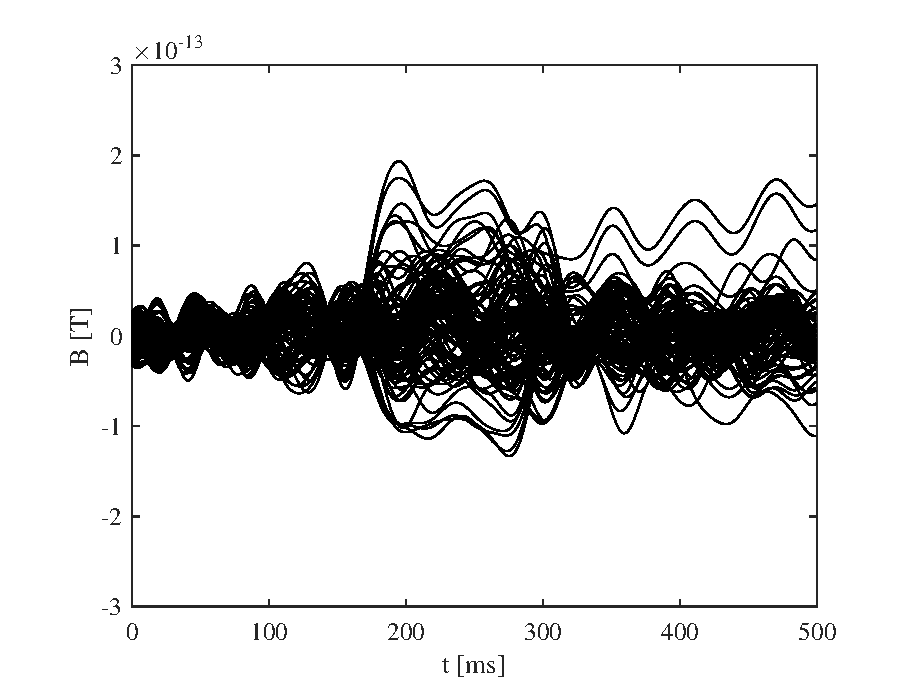
\includegraphics[width=\textwidth]{ergebnisse/butterfly/pa10a1_eve2_raw_mag_butterfly.eps}
    \subcaption{VP \texttt{pa10}, Rohdaten}
    \label{img:butterfly:mag:raw:pa10}
  \end{subfigure}\hspace*{0.08\textwidth}
  %
  \begin{subfigure}[c]{0.36\textwidth}
    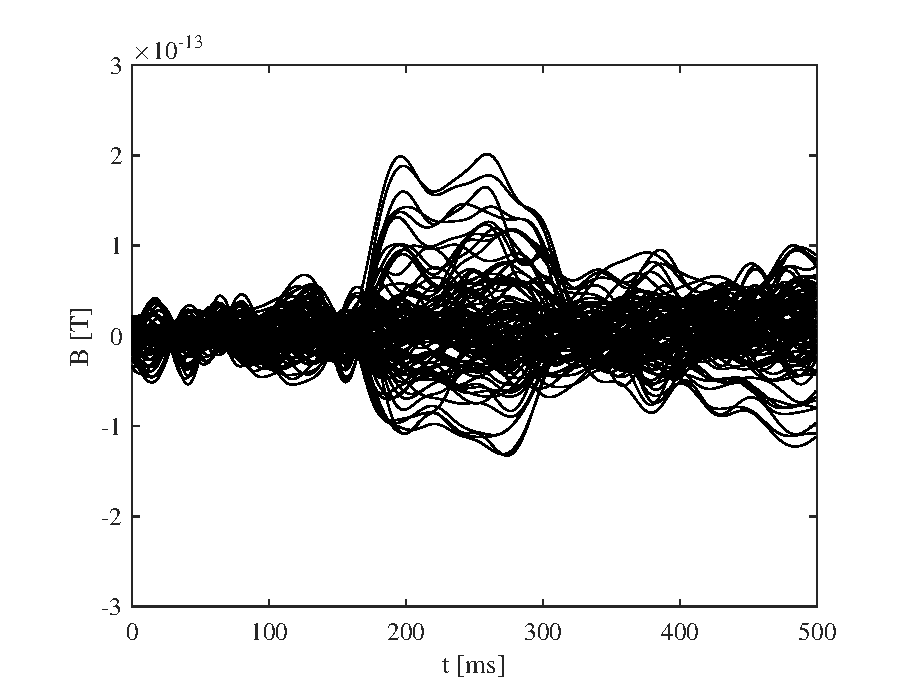
\includegraphics[width=\textwidth]{ergebnisse/butterfly/pa10a1_eve2_sss_mag_butterfly.eps}
    \subcaption{VP \texttt{pa10}, SSS-Daten}
    \label{img:butterfly:mag:sss:pa10}
  \end{subfigure}
  %
  \vspace*{3mm}
  \captionsetup{justification=justified}
  \caption[Gemessene Aktivität an den Magnetometern]{Gemessene Aktivität an den Magnetometern für beide Versuchspersonen, jeweils in Block 1 mit Rohdaten und SSS-Daten.}
  \label{img:butterfly:mag}
\end{figure}

Im Folgenden soll noch eine letzte Vorbetrachtung erfolgen. In den Abbildungen \ref{img:butterfly:grad} und \ref{img:butterfly:mag} sind die Aktivitäten der Kanäle der Versuchspersonen für Block 1 für Rohdaten und SSS-Daten aufgetragen, getrennt für Gradiometer und Magnetometer. Da die Verläufe für MC-Daten eine hohe Ähnlichkeit mit denen der SSS-Daten aufweisen und sich die Aktivitäten auch in den anderen Blöcken analog verhalten, wurden sie hier nicht gezeigt, ein Vergleich zwischen Rohdaten und SSS-Daten für Block 1 soll an dieser Stelle genügen. Abgebildet sind bereits die vorverarbeiteten Daten. Vor allem bei den Rohdaten ist also zu berücksichtigen, dass die schlechtesten Trials bei der Mittelung nicht berücksichtigt wurden.

Es ist zu erkennen, dass ein Maximum der Aktivität um ca. $210\,ms$ liegen muss. Diese Aktivität entspricht der MMNm. Weitere kleine Ausschläge können u.U. noch nach $300\,ms$ vorkommen, sollten jedoch nicht stärker relevant sein. Bei Versuchsperson \texttt{pa10} fällt auf, dass sowohl in den Gradiometern, also auch den Magnetometern, eine etwas verzerrte Aktivität zwischen $200\,ms$ und $300\,ms$ vorliegt (Abbildungen~\ref{img:butterfly:grad:raw:pa10},~\ref{img:butterfly:grad:sss:pa10},~\ref{img:butterfly:mag:raw:pa10} und~\ref{img:butterfly:mag:sss:pa10}). Außerdem wird in den Daten erneut deutlich (wie schon bei der Frequenzanalyse), dass die Rekonstruktionsverfahren bei den Rohdaten eine gewisse Leistung zu erbringen haben, da das Rauschen nicht unerheblich ist. Bei den Rohdaten kommt es zu auseinander laufenden Aktivitäten, die sich äußerst unsystematisch verhalten, vor allem bei den Gradiometern deutlich zu sehen (Abbildung~\ref{img:butterfly:grad:raw:pa07} und~\ref{img:butterfly:grad:raw:pa10}).

\subsection{Quellrekonstruktionen und Zeitverläufe}

Bei der Quellrekonstruktion waren die Ergebnisse von den Versuchspersonen \texttt{pa07} und \texttt{pa10} weitestgehend analog. Es wird im folgenden überwiegende auf die Ergebnisse von \texttt{pa07} zurückgegriffen und nur in nötigen Fällen ein Vergleich mit \texttt{pa10} angestellt.

\subsubsection{Lateralität}

Die zentrale Amplitude der MMNm konnte bei $208\,ms$ registriert werden. Bei beiden Versuchspersonen kam es zu einer rechtsseitigen Lateralität. In der topografischen Darstellung der Sensoren in den Abbildungen in~\ref{img:topolot} wird die bevorzugte rechtsseitige Aktivität deutlich. Die Sensoraktivität wurde im Intervall von  $203\,ms$ bis $213\,ms$ gemittelt.

\begin{figure}
  \centering
  \captionsetup{justification=centering}
  %
  \begin{subfigure}[c]{0.47\textwidth}
    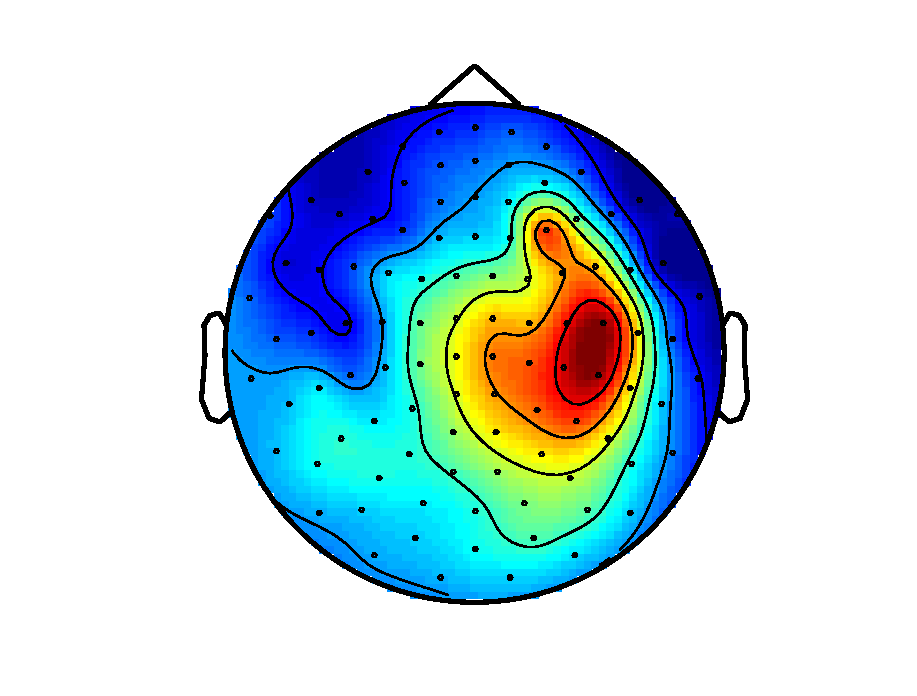
\includegraphics[width=\textwidth]{ergebnisse/topoplot/pa07a1_raw.eps}
    \subcaption{Versuchsperson \texttt{pa07}}
    \label{img:topolot:pa07a1}
  \end{subfigure}\hspace*{0.04\textwidth}
  %
  \begin{subfigure}[c]{0.47\textwidth}
    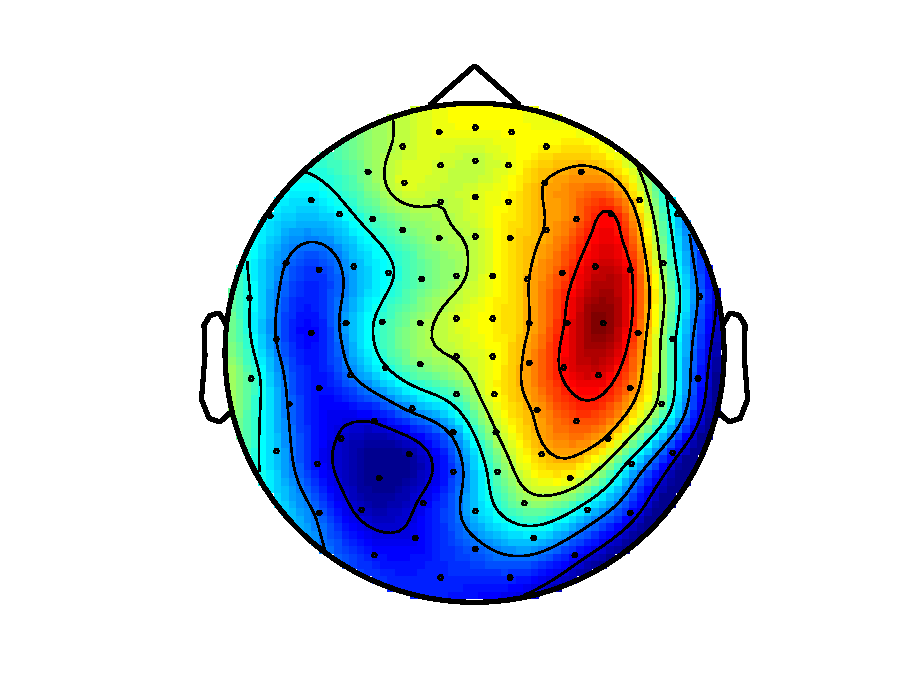
\includegraphics[width=\textwidth]{ergebnisse/topoplot/pa10a1_raw.eps}
    \subcaption{Versuchsperson \texttt{pa10}}
    \label{img:topolot:pa10a1}
  \end{subfigure}
  %
  \captionsetup{justification=justified}
  \vspace*{3mm}
  \caption[Topografische Darstellung der Sensoraktivität zum Zeitpunkt des Auftretens der MMNm]{Topografische Darstellung der Sensoraktivität zum Zeitpunkt des Auftretens der MMNm. Es wurde ein Intervall von $\pm5\,ms$ um den Zeitpunkt $208\,ms$ gemittelt. Verwendet wurden Rohdaten und die Aktivität ist jeweils für Block~1 gezeigt. Blaue Bereiche kennzeichnen Gebiete mit negativer magnetischer Flussdichte, in die das Magnetfeld eindringt. Rote Bereiche kennzeichnen Gebiete mit positiver Flussdichte, aus denen das Magnetfeld heraus tritt.}
  \label{img:topolot}
\end{figure}

Die lateralisierte Aktivität an den Sensoren sollte sich auch in der rekonstruierten Aktivität zeigen. Unter Verwendung von Minimum Norm Estimate wird die Lateralisierung deutlich. Abbildungen~\ref{img:activity-latera:mne:left} und~\ref{img:activity-latera:mne:right} zeigen die rekonstruierte Aktivität von Minimum Norm Estimate bei Versuchsperson \texttt{pa07} auf Basis der Rohdaten. Beamformer scheint hier Probleme zu haben die lateralisierte Aktivität zu erkennen. Abbildungen~\ref{img:activity-latera:lcmv:left} und~\ref{img:activity-latera:lcmv:right} zeigen eine eher gleichmäßige Aktivität auf beiden Hemisphären. Etwas mehr Aktivität scheint laut Beamformer sogar in der linken Hemisphäre zu sein, was den gemessene Aktivitäten an den Sensoren widerspricht.

\begin{figure}
  \centering
  \captionsetup{justification=centering}
  %
  \begin{subfigure}[c]{0.47\textwidth}
    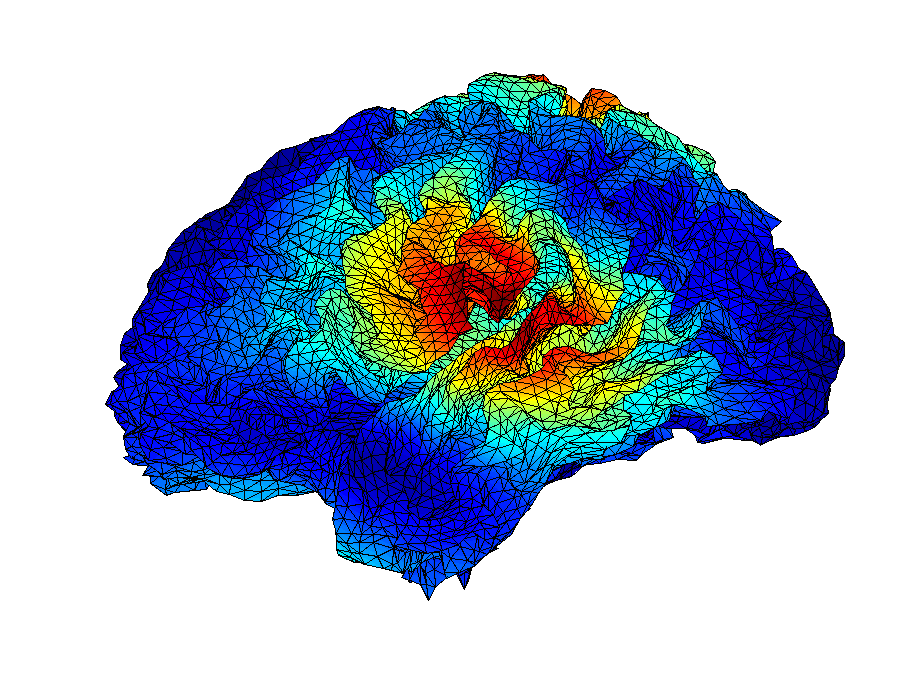
\includegraphics[width=\textwidth]{ergebnisse/activity/pa07_eve2_raw_lcmv_activity_left.eps}
    \subcaption{LCMV Beamformer, linke Hemisphäre}
    \label{img:activity-latera:lcmv:left}
  \end{subfigure}\hspace*{0.04\textwidth}
  %
  \begin{subfigure}[c]{0.47\textwidth}
    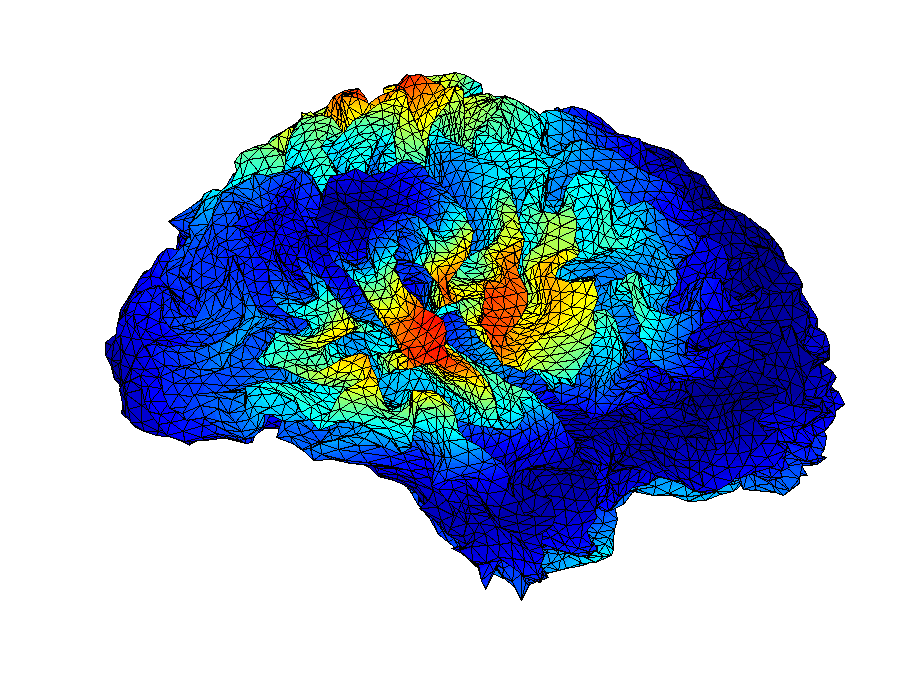
\includegraphics[width=\textwidth]{ergebnisse/activity/pa07_eve2_raw_lcmv_activity_right.eps}
    \subcaption{LCMV Beamformer, rechte Hemisphäre}
    \label{img:activity-latera:lcmv:right}
  \end{subfigure}  
  \vspace*{0.04\textwidth}
  \begin{subfigure}[c]{0.47\textwidth}
    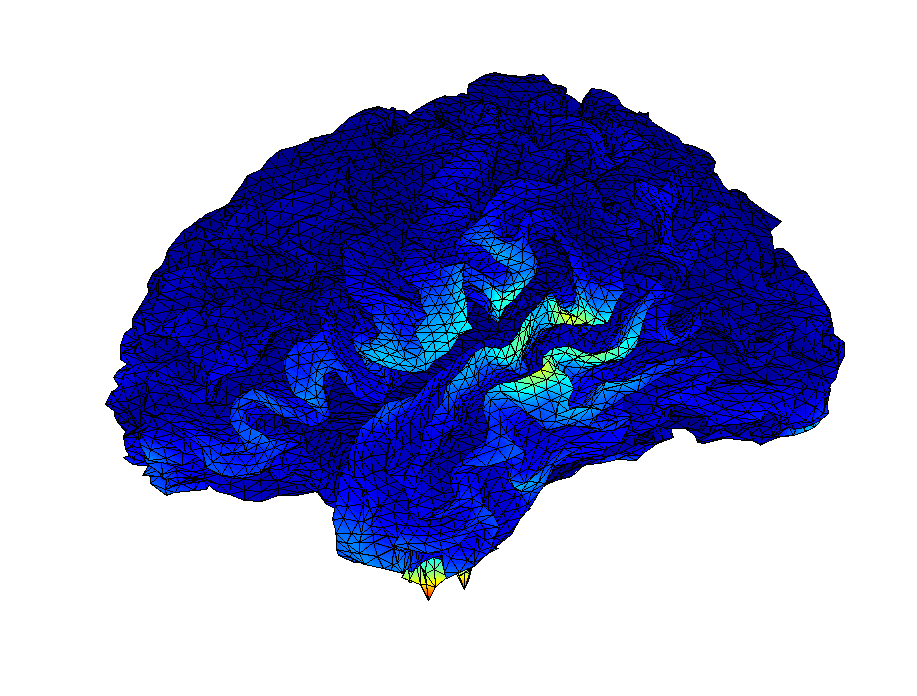
\includegraphics[width=\textwidth]{ergebnisse/activity/pa07_eve2_raw_mne_activity_left.eps}
    \subcaption{Minimum Norm Estimate, links Hemisphäre}
    \label{img:activity-latera:mne:left}
  \end{subfigure}\hspace*{0.04\textwidth}
  %
  \begin{subfigure}[c]{0.47\textwidth}
    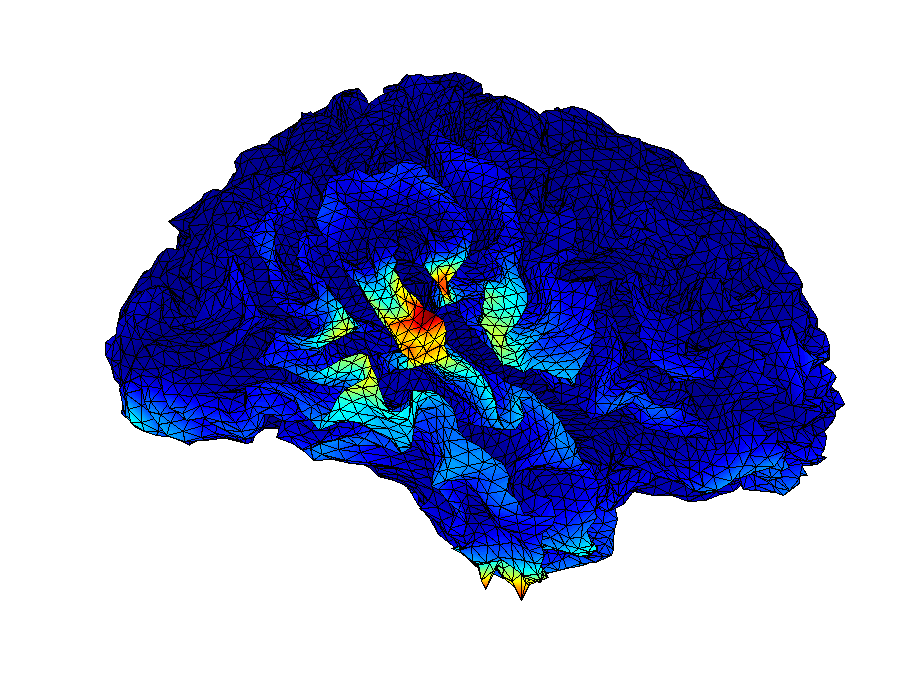
\includegraphics[width=\textwidth]{ergebnisse/activity/pa07_eve2_raw_mne_activity_right.eps}
    \subcaption{Minimum Norm Estimate, rechte Hemisphäre}
    \label{img:activity-latera:mne:right}
  \end{subfigure}
  %
  \captionsetup{justification=justified}
%  \vspace*{3mm}
  \caption[Quellaktivität bei Versuchsperson \texttt{pa07} auf Basis der Rohdaten.]{Quellaktivität bei Versuchsperson \texttt{pa07} auf Basis der Rohdaten. Jeweils die rechte und linke Hemisphäre, berechnet von LCMV Beamformfer und Minimum Norm Estimate.}
  \label{img:activity-lateral}
\end{figure}

\subsubsection{Scheinquellen}

Während Minimum Norm Estimate eine Quellaktivität nur rechts und links errechnet, erscheint in den Ergebnissen der Beamformer-Lösung auch an der oberen Seite des Kopfes Aktivität. Deutlich zu sehen in Abbildungen~\ref{img:activity-latera:lcmv:left} und Abbildungen~\ref{img:activity-latera:lcmv:right}. Aber auch unter Verwendung von SSS- und Rohdaten bleibt diese Aktivität bei der Beamformer-Lösung bestehen, wie in Abbildungen~\ref{img:pa07:aktiv:raw-lcmv},~\ref{img:pa07:aktiv:sss-lcmv} und~\ref{img:pa07:aktiv:mc-lcmv} zu sehen. Die Studie, auf der die Daten basieren, gibt keinen Hinweis auf eine Aktivität im Frontal- oder Parietallappen. MMNm-Aktivität ist nur im Temporallappen zu erwarten.

Eine mögliche Erklärung für diese Quellen ist das Auftreten von Scheinquellen bzw. \emph{Ghost Sources} \parencite{trujillo2004bayesian}. Sie bezeichnen Dipole, die zwar aus Sicht des Rekonstruktionsverfahrens logisch sind, aber nicht real existieren. Dipole, d.h. mögliche Quellen, liegen senkrecht zu den Gradienten des Magnetfeldes. Besonders an denen Stellen, an denen der Gradient sehr steil ist. In Abbildung~\ref{img:topolot} sind das die Bereiche in denen sehr rote (positive magnetische Flussdichte) und sehr blaue (negative magnetische Flussdichte) Bereiche nah aneinander liegen. In den roten Bereichen treten die Feldlinien des Magnetfeldes aus dem Gehirn aus, in den blauen Bereichen treten sie wieder ein. Eine starke Quelle (bzw. ein Strom) sollte also in der genannten Abbildung beispielsweise im rechten temporalen Bereich entlang der Höhenlinien von unten nach oben liegen. Diese wurde sowohl von Beamformer, als auch von Minimum Norm Estimate zuverlässig gefunden. Eine weitere reale Quelle liegt im linken Bereich von innen nach außen, an der Grenze zwischen hellblau und dunkelblau. Diese Quelle sollte eher schwach sein. In diesem Fall errechnet Minimum Norm Estimate eine relativ präzise Voraussage, Beamformer überschätzt die Aktivität in diesem Bereich deutlich, wenn die entsprechenden Annahmen über das Auftreten der MMNm korrekt sind. Im mittleren vorderen Bereich kommt es ebenfalls zu einer Grenze. Diese Grenze entsteht aber in der Realität nicht durch einen Strom, sondern durch die entgegengesetzten Ströme auf der rechten und linken Seite. Während Minimum Norm Estimate hier korrekt erkennt, dass es sich nicht um eine wirklich Quelle handelt, schätzt Beamformer hier eine Quelle. Tatsächlich wäre eine Quelle physikalisch möglich, es kann aber begründet davon ausgegangen werden, dass sie in der Realität nicht vorliegt. Es handelt sich um eine durch Ghost Sources ausgelöste Scheinaktivität.

\begin{figure}
%  \centering
  \captionsetup{justification=centering}
  %
  \begin{subfigure}[c]{0.47\textwidth}
    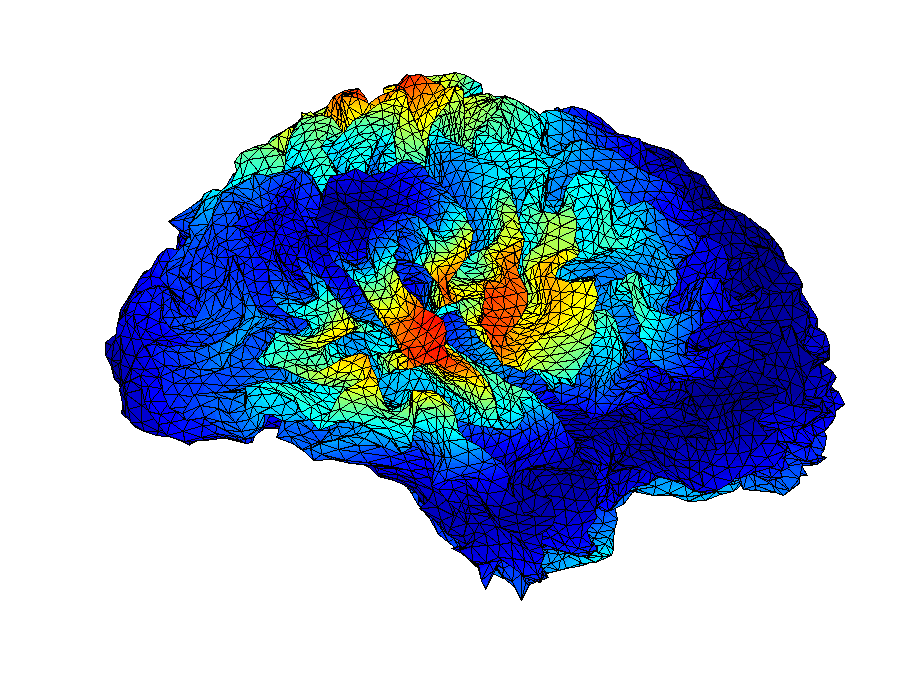
\includegraphics[width=\textwidth]{ergebnisse/activity/pa07_eve2_raw_lcmv_activity_right.eps}
    \subcaption{LCMV Beamformer, Rohdaten}
    \label{img:pa07:aktiv:raw-lcmv}
  \end{subfigure}\hspace*{0.04\textwidth}
  %
  \begin{subfigure}[c]{0.47\textwidth}
    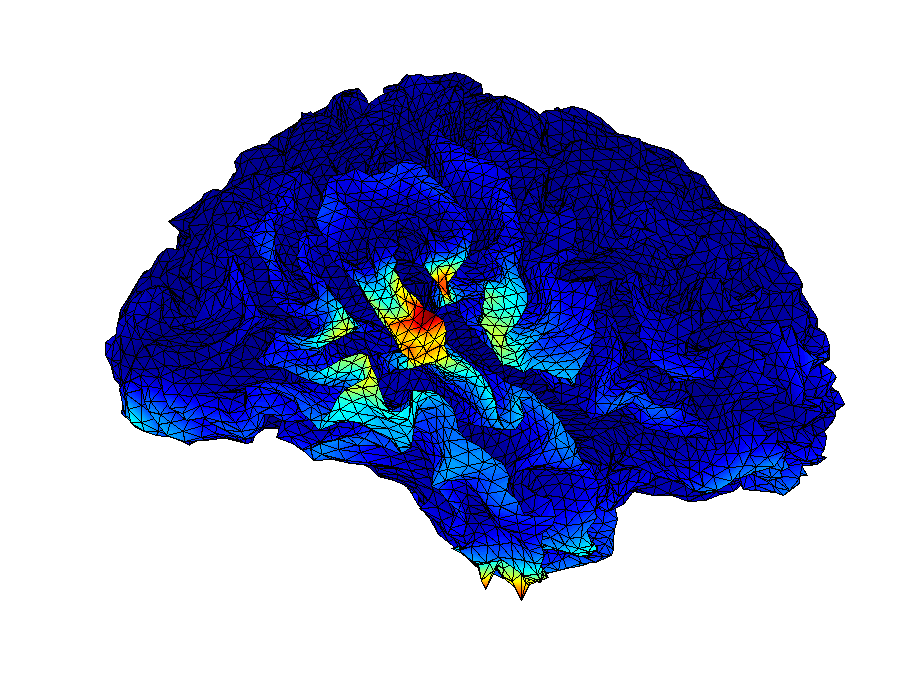
\includegraphics[width=\textwidth]{ergebnisse/activity/pa07_eve2_raw_mne_activity_right.eps}
    \subcaption{Minimum Norm Estimate, Rohdaten}
    \label{img:pa07:aktiv:raw-mne}
  \end{subfigure}\vspace*{0.04\textwidth}
  %
  \begin{subfigure}[c]{0.47\textwidth}
    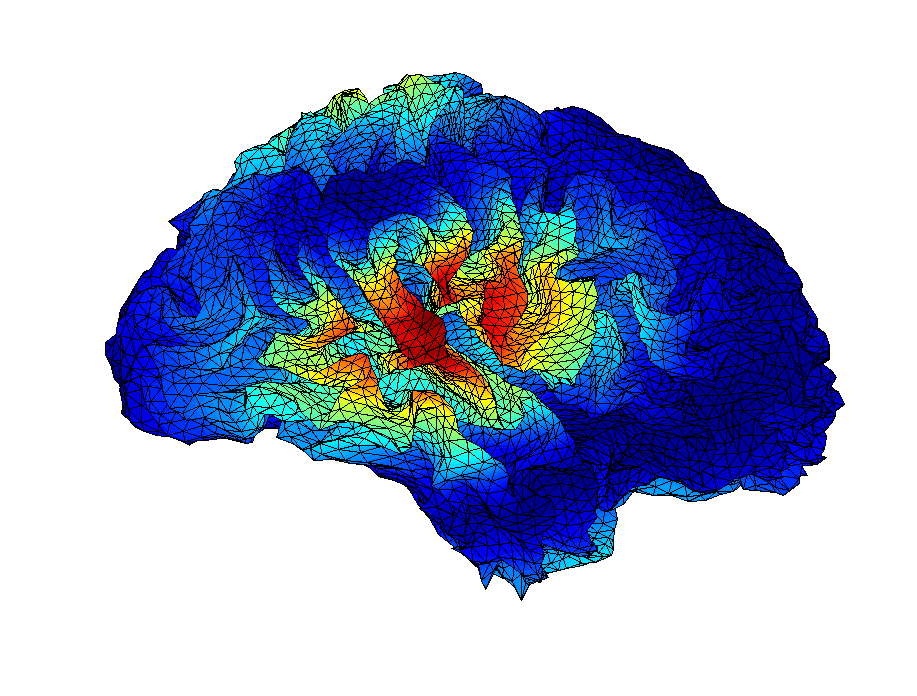
\includegraphics[width=\textwidth]{ergebnisse/activity/pa07_eve2_sss_lcmv_activity_right.eps}
    \subcaption{LCMV Beamformer, SSS-Daten}
    \label{img:pa07:aktiv:sss-lcmv}
  \end{subfigure}\hspace*{0.04\textwidth}
  %
  \begin{subfigure}[c]{0.47\textwidth}
    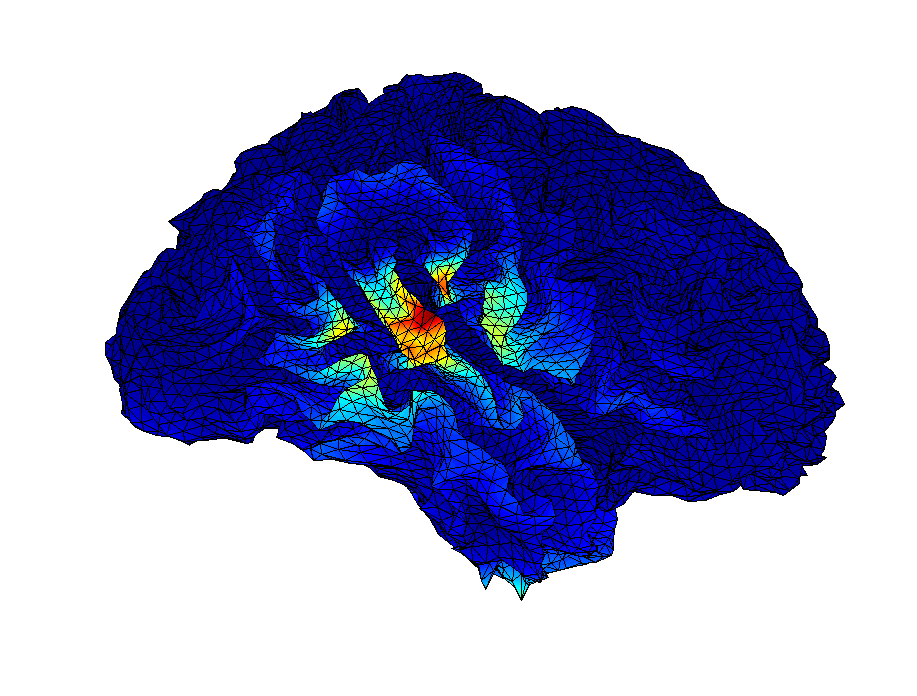
\includegraphics[width=\textwidth]{ergebnisse/activity/pa07_eve2_sss_mne_activity_right.eps}
    \subcaption{Minimum Norm Estimate, SSS-Daten}
    \label{img:pa07:aktiv:sss-mne}
  \end{subfigure}\vspace*{0.04\textwidth}
  %
  \begin{subfigure}[c]{0.47\textwidth}
    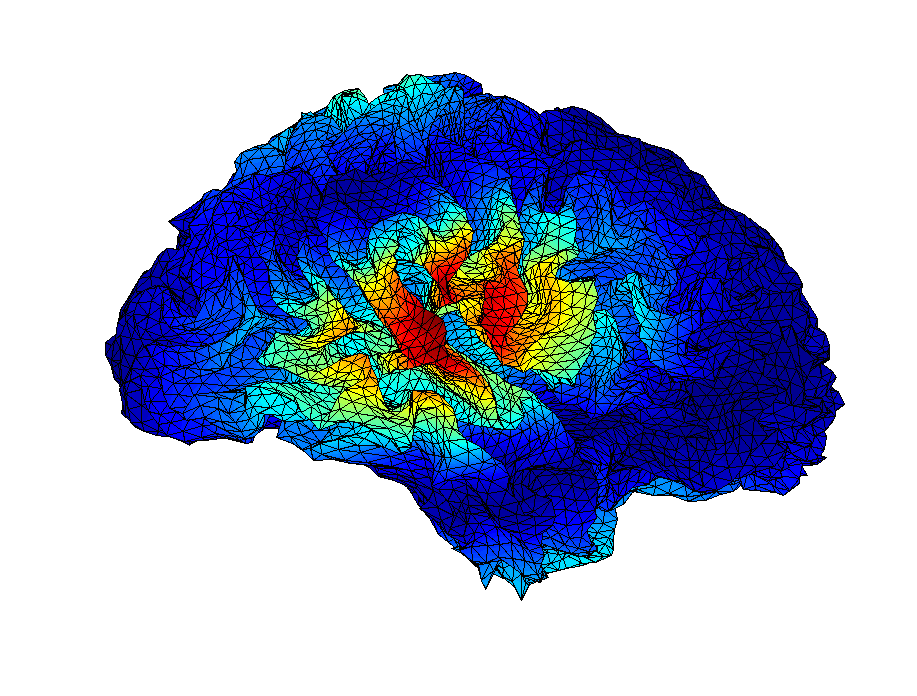
\includegraphics[width=\textwidth]{ergebnisse/activity/pa07_eve2_mc_lcmv_activity_right.eps}
    \subcaption{LCMV Beamformer, MC-Daten}
    \label{img:pa07:aktiv:mc-lcmv}
  \end{subfigure}\hspace*{0.05\textwidth}
  %
  \begin{subfigure}[c]{0.47\textwidth}
    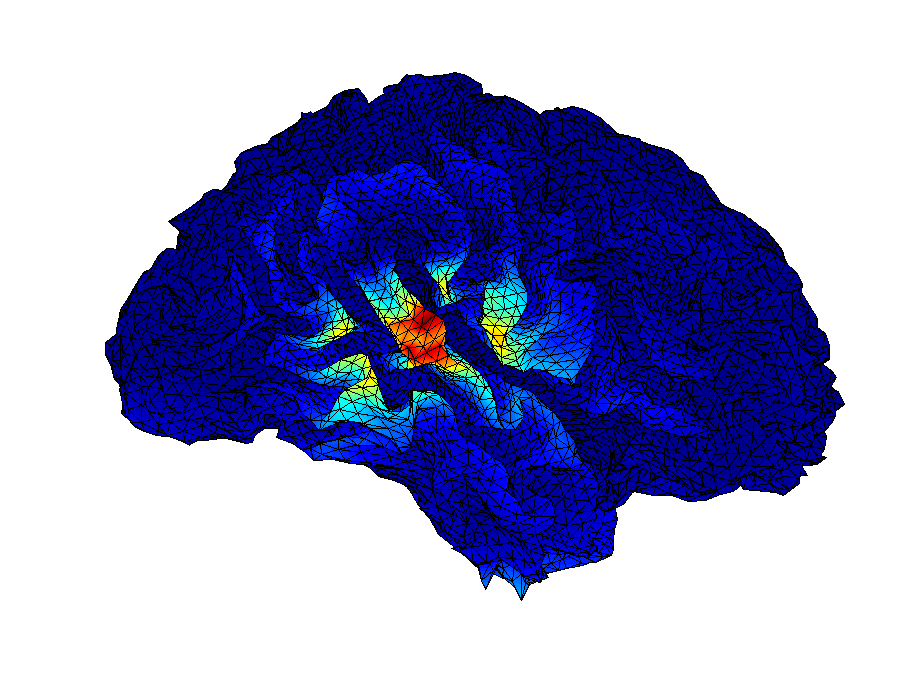
\includegraphics[width=\textwidth]{ergebnisse/activity/pa07_eve2_mc_mne_activity_right.eps}
    \subcaption{Minimum Norm Estimate, MC-Daten}
    \label{img:pa07:aktiv:mc-mne}
  \end{subfigure}
  %
  \captionsetup{justification=justified}
  \vspace*{3mm}
  \caption[Quellaktivität von Versuchsperson \texttt{pa07}]{Quellaktivität von Versuchsperson \texttt{pa07} in allen Bedingungen in der linken Hemisphäre bei $208\,ms$ zum Zeitpunkt des Auftretens der MMNm.}
  \label{img:pa07:aktiv}
\end{figure}

\subsubsection{Aktivitätsverteilung}
\label{sec:akti-verteilung}
%%% Verteilung/Konzentrationsgrad für pa07, pa10

Die Verteilung der Aktivität bei Beamformer und Minimum Norm Estimate weisen unterschiedliche Eigenschaften auf. Während bei Minimum Norm Estimate der Bereich der Aktivität sehr konzentriert Auftritt, weist Beamformer ein großes Areal an Aktivität auf. Mit Hilfe ...

%%% Verteilungskenngröße ergänzen, wie berechnet? Was sagt das Maß aus?

\subsubsection{Rauschunterdrückte Daten}

Unter Verwendung rauschunterdrückter Daten zeigen beide Verfahren bessere Ergebnisse. Während die Verbesserungen bei Minimum Norm Estimate eher minimal sind, nimmt bei Beamformer die Scheinaktivität im Parietallappen ab. Dieses Verhalten wird in den Abbildungen~\ref{img:pa07:aktiv:raw-lcmv} bis~\ref{img:pa07:aktiv:mc-mne} deutlich. Die Ergebnisse würde also an dieser Stelle der Hypothese widersprechen. Nach Auswertung der Verteilung der Quellaktivität zum Zeitpunkt des Auftretens der MMNm scheint Beamformer unter Verwendung der Rohdaten keine guten Lösungen zu liefern, während Minimum Norm Estimate entgegen der Nebenhypothese relativ gute Lösung errechnen kann. Da die Aktivitäten in den Abbildungen nicht einheitlich skaliert sind, ist eine weitere Betrachtung unter Normierung nötig. Außerdem ist es nötig auch die anderen Zeitpunkt zu betrachten, um die Qualität der Lösungen abschätzen zu können.

\subsubsection{Zeitverläufe}

\begin{figure}
%  \centering
  \captionsetup{justification=centering}
  %
  \begin{subfigure}[c]{0.47\textwidth}
    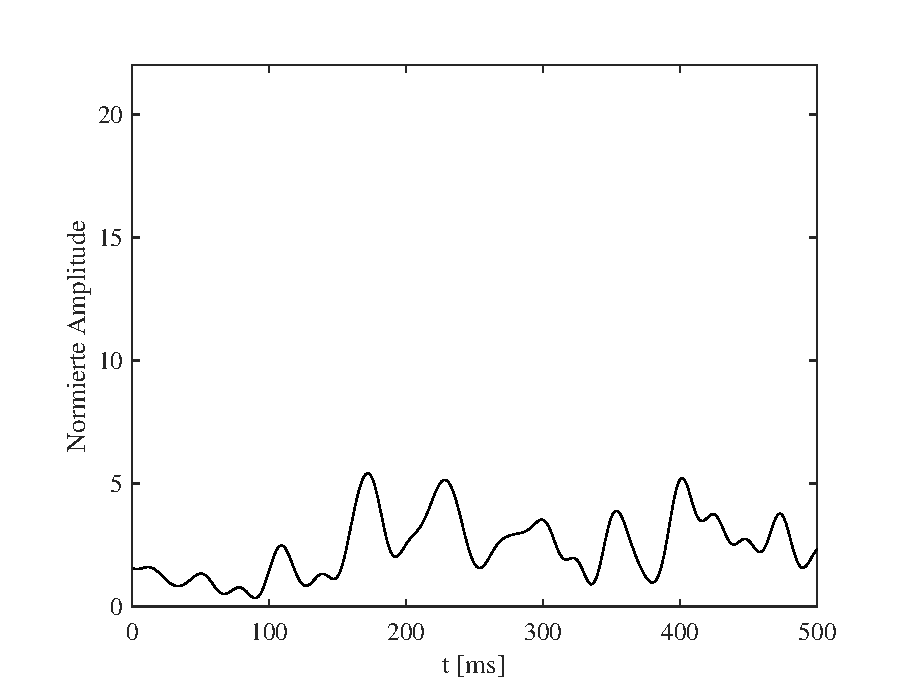
\includegraphics[width=\textwidth]{ergebnisse/timecourse/pa07_eve2_raw_lcmv_timecourse_right.eps}
    \subcaption{LCMV Beamformer, Rohdaten}
    \label{img:pa07:zeit:raw-lcmv}
  \end{subfigure}\hspace*{0.04\textwidth}
  %
  \begin{subfigure}[c]{0.47\textwidth}
    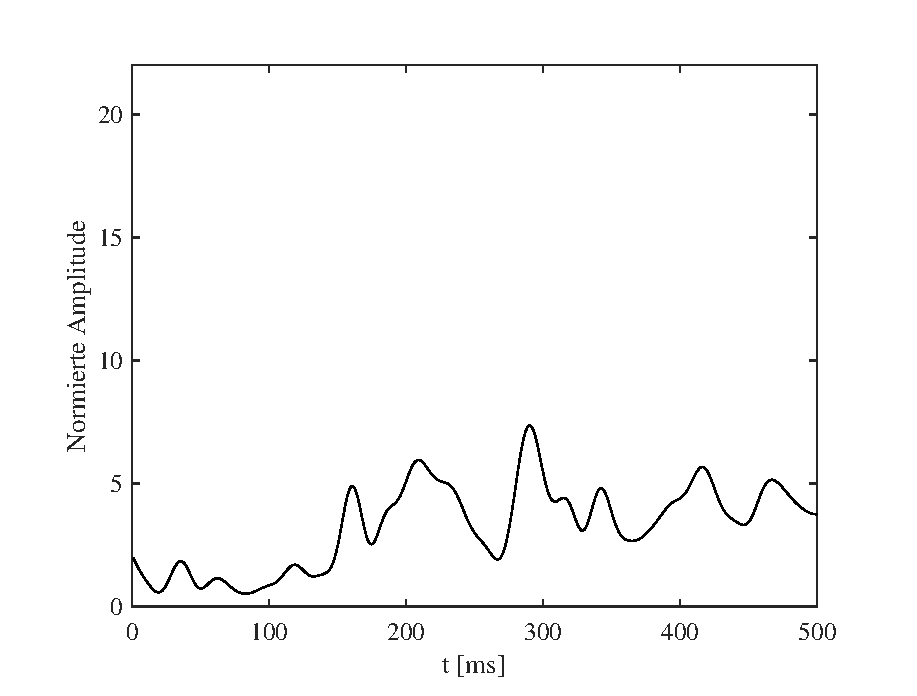
\includegraphics[width=\textwidth]{ergebnisse/timecourse/pa07_eve2_raw_mne_timecourse_right.eps}
    \subcaption{Minimum Norm Estimate, Rohdaten}
    \label{img:pa07:zeit:raw-mne}
  \end{subfigure}\vspace*{0.04\textwidth}
  %
  \begin{subfigure}[c]{0.47\textwidth}
    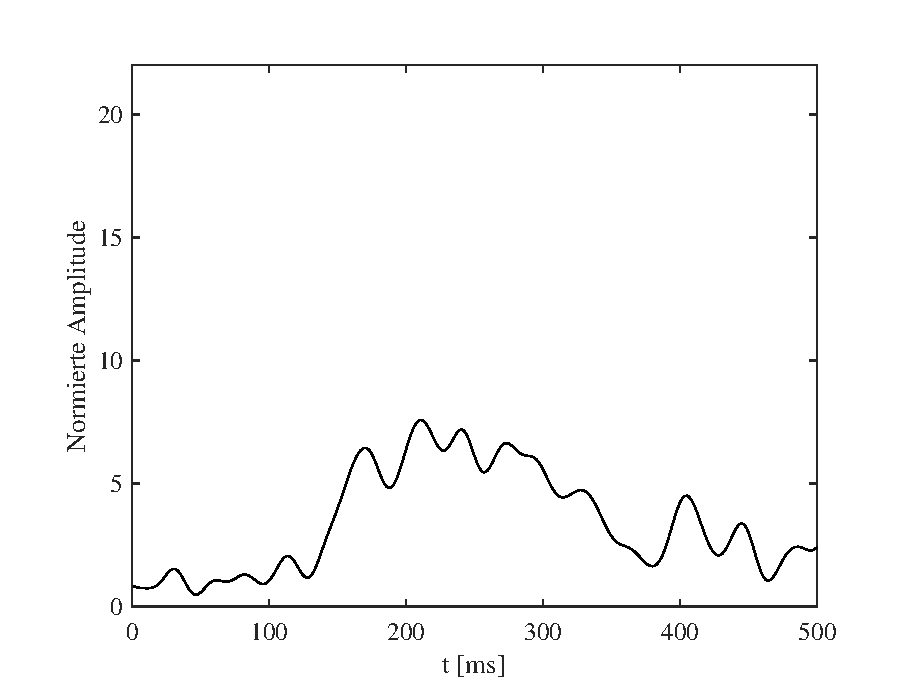
\includegraphics[width=\textwidth]{ergebnisse/timecourse/pa07_eve2_sss_lcmv_timecourse_right.eps}
    \subcaption{LCMV Beamformer, SSS-Daten}
    \label{img:pa07:zeit:sss-lcmv}
  \end{subfigure}\hspace*{0.04\textwidth}
  %
  \begin{subfigure}[c]{0.47\textwidth}
    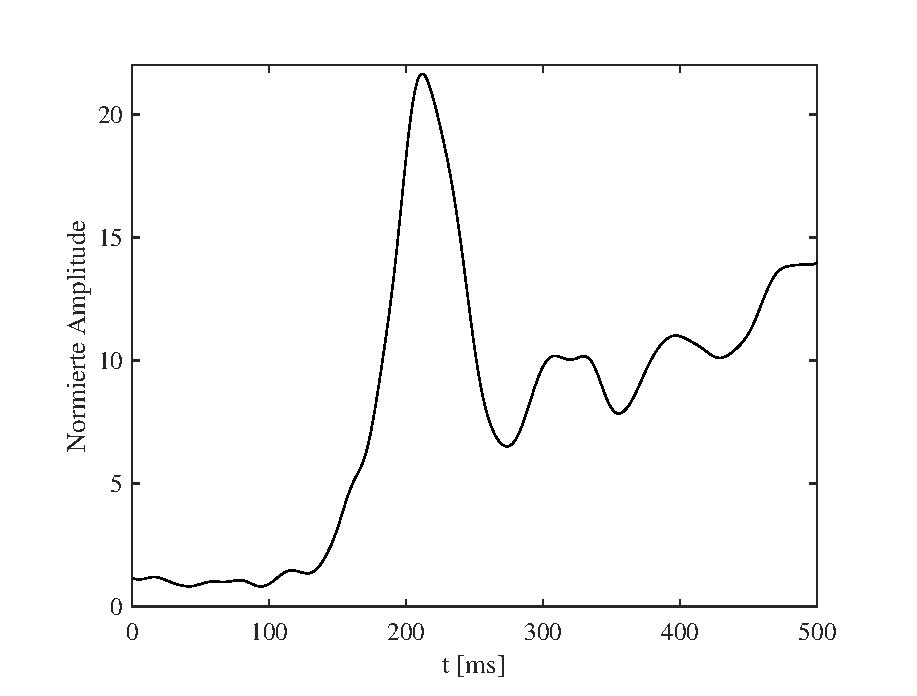
\includegraphics[width=\textwidth]{ergebnisse/timecourse/pa07_eve2_sss_mne_timecourse_right.eps}
    \subcaption{Minimum Norm Estimate, SSS-Daten}
    \label{img:pa07:zeit:sss-mne}
  \end{subfigure}\vspace*{0.04\textwidth}
  %
  \begin{subfigure}[c]{0.47\textwidth}
    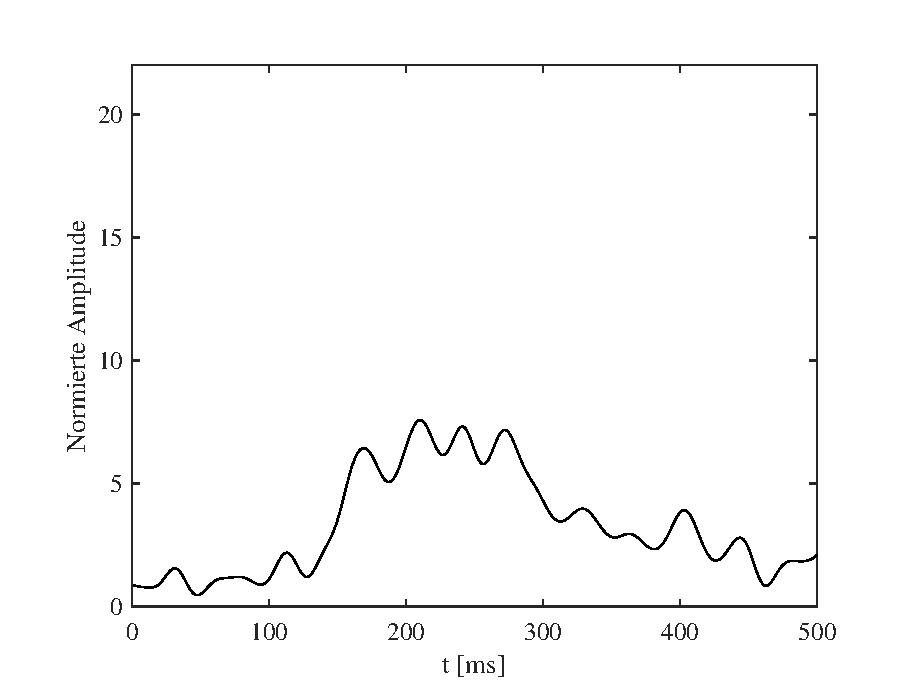
\includegraphics[width=\textwidth]{ergebnisse/timecourse/pa07_eve2_mc_lcmv_timecourse_right.eps}
    \subcaption{LCMV Beamformer, MC-Daten}
    \label{img:pa07:zeit:mc-lcmv}
  \end{subfigure}\hspace*{0.05\textwidth}
  %
  \begin{subfigure}[c]{0.47\textwidth}
    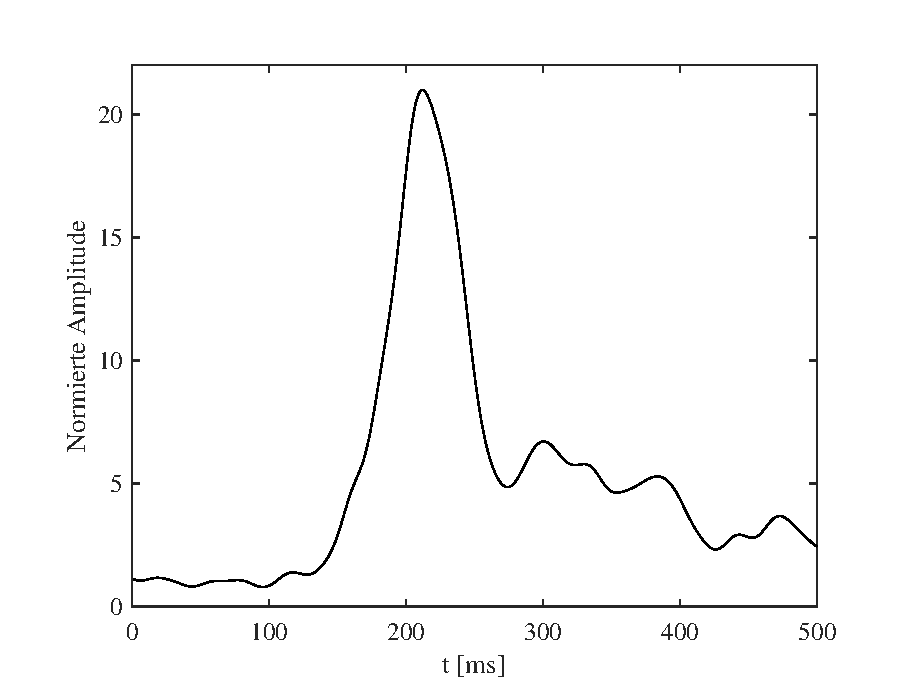
\includegraphics[width=\textwidth]{ergebnisse/timecourse/pa07_eve2_mc_mne_timecourse_right.eps}
    \subcaption{Minimum Norm Estimate, MC-Daten}
    \label{img:pa07:zeit:mc-mne}
  \end{subfigure}
  %
  \captionsetup{justification=justified}
  \vspace*{3mm}
  \caption[Zeitverlauf der Aktivität von Versuchsperson \texttt{pa07}]{Zeitverlauf der Aktivität von Versuchsperson \texttt{pa07} in allen Bedingungen im Gyrus temporalis superior.}
  \label{img:pa07:zeit}
\end{figure}

Für die Berechnung der Zeitverläufe wurde zunächst die Aktivität aller Quellen gemittelt. Dabei wurden nur solche Quellen berücksichtigt, die im auditiven Kortex, d.h. im Gyrus temporalis superior liegen (siehe auch Abschnitt \nameref{sec:audicort} auf Seite~\pageref{sec:audicort}). Da die Quellaktivität der beiden Lösungen unterschiedlich zu interpretieren ist und in unterschiedlichen Größenordnungen liegt (siehe auch Abschnitt \nameref{sec:amplitud} auf Seite~\pageref{sec:amplitud}), wurde der Zeitverlauf zusätzlich normiert. Dafür wurde der Mittelwert der Aktivität in der Baseline verwendet, d.h. in den ersten $100\,ms$. Jeder Wert im Zeitverlauf wurde durch die mittlere Baseline geteilt. Die Signalaktivität wurde ins Verhältnis zur Rauschaktivität gesetzt. Die Ergebnisse für Versuchsperson \texttt{pa07} für alle Bedingungen sind in Abbildung~\ref{img:pa07:zeit} dargestellt.

In den Zeitverläufen werden zwei Ergebnisse deutlich. Zum einen weist Minimum Norm Estimate im Zeitverlauf unter Verwendung von Rohdaten keine MMNm-Amplitude auf (siehe Abbildung~\ref{img:pa07:zeit:raw-mne}). Zwar ist die Aktivität wie oben beschrieben genauer, der Zeitverlauf weist jedoch nicht das Verhalten auf, was im Gyrus temporalis superior für eine MMNm zu erwarten wäre. Die Nebenhypothese kann an dieser Stelle also teilweise bestätigt werden. Minimum Norm Estimate zeigt keine gute Lösung unter Verwendung von Rohdaten. Das andere Ergebnis ist, dass Beamformer einen typischen Zeitverlauf auch unter Verwendung von rauschunterdrückten Daten nicht errechnen kann (siehe Abbildungen~\ref{img:pa07:zeit:sss-lcmv} und~\ref{img:pa07:zeit:mc-lcmv}).

Ein drittes Merkmal ist der Unterschied zwischen der Verwendung von SSS- und MC-Daten. In der Minimum Norm Estimate Lösung zeigen sich Unterschiede, die konsistent auch bei Versuchsperson \texttt{pa10} auftreten. Nach der Amplitude kommt es bei der Verwendung von SSS-Daten zu einer bleibenden Aktivität auf relativ hohem Niveau (siehe Abbildung~\ref{img:pa07:zeit:sss-mne}). Bei der Verwendung von MC-Daten ist dieses Plateau unterdrückt (siehe Abbildung~\ref{img:pa07:zeit:mc-mne}). Dies könnte mit der Bewegung der Versuchsperson innerhalb eines Blocks zusammen hängen, die nur bei MC korrigiert wird. Da diesbezüglich jedoch zu wenige Daten vorliegen und eine systematische Bewegung im Versuch nicht durchgeführt wurde, kann eine weitere Analyse dieses Merkmals an der Stelle nicht erfolgen.

% #######################
% ##### DISKUSSION  #####
% #######################

\newpage

\section{Diskussion}
\label{sec:diskussion}

Die Ergebnisse zeigen deutlich, dass LCMV Beamformer, aber auch Minimum Norm Estimate ohne Anwendung eines vorhergehenden Rauschunterdrückungsverfahrens keine adäquaten Lösungen liefern. Die Hypothese kann verworfen, die Nebenhypothese größtenteils aufrecht erhalten werden. Zusätzlich zu diesem Ergebnis wurde deutlich, dass Beamformer auch unter Verwendung rauschunterdrückter Daten keine guten Lösungen liefert. Um zu verstehen, warum Beamformer bei der Berechnung der Lösungen so große Probleme hatte, müssen die Annahmen über Beamformer genauer analysiert werden.

\subsection{Vorverarbeitung}

Wichtig bei der Interpretation der Ergebnisse ist die Tatsache, dass Trials mit einer magnetischen Flussdichte, einem Gradienten oder einer Augenaktivität (gemessen mittels EOG) über einem gewissen Grenzwert verworfen wurden. In Tabelle \ref{tab:rejecting} war die entsprechende Anzahl der verwendeten Trials aufgelistet. Da innerhalb der Rohdaten häufiger Abweichungen über die Grenzwerte hinaus auftraten, wurden hier entsprechend mehr Trials verworfen. Es ist nicht falsch zu behaupten, dass dies einer gewissen, wenn auch äußerst vereinfachten, Rauschunterdrückung entspricht. Zeitpunkte an denen besonders hohes Rauschen auftrat wurden einfach nicht berücksichtigt. Die deutlich geringere Anzahl der verwendeten Trials in den Rohdaten könnte einen Einfluss auf die Berechnung der Lösungen beider Verfahren gehabt haben, der z.B. Einfluss auf den Rangdefekt der Kovarianzmatrix haben könnte (siehe auch Abschnitt \nameref{sec:regu-kov}). Denkbar wäre auch, dass von dieser Reduzierung Beamformer stärker betroffen ist als Minimum Norm Estimate.

Da es sich jedoch um ein Standardverfahren für die Verarbeitung der SSS- und MC-Daten handelt, war es aus Gründen der Vergleichbarkeit angebracht, auch die Rohdaten entsprechend zu verarbeiten. Trotzdem wäre es an dieser Stelle interessant zu untersuchen, wie sich die Verfahren verhalten würden, wenn ausnahmslos alle Trials verwendet werden oder der Grenzwert liberaler gewählt wird.

\subsection{Korreliertheit der Aktivität}

Die Annahmen der Verfahren in der Hypothesenbildung waren nicht ganz vollständig, was vermutlich zu der falschen Vorhersage geführt hat. Ein Problem des Beamformer-Verfahrens ist die Annahme der Unkorreliertheit der Quellaktivität. Dies wurde im Abschnitt \nameref{sec:beam} ab Seite~\pageref{sec:beam} zwar ausführlich diskutiert, nicht aber hinreichend in der Hypothese berücksichtigt. Die Quellen der Aktivitäten innerhalb des Gehirns sind entgegen der Annahme vermutlich sogar sehr stark korreliert. Dabei liegt eine Korrelation nicht nur bei nächsten Nachbarn vor, sondern auch auf beiden Hemisphären, da beide Ohren gleichzeitig stimuliert wurden. Auf der anderen Seite wurde bei Minimum Norm Estimate die Eigenschaft des Ansatzes der minimalen Energie unterschätzt. Wahrscheinlich führt gerade diese Annahme dazu, dass der Einfluss weit entfernter Störquellen eher unterdrückt wird.

\subsection{Regularisierung der Kovarianzmatrix}
\label{sec:regu-kov}

Problematisch ist bei Beamformer auch der Umgang mit ereigniskorrelierten Feldern~(ERF), diskutiert in \textcite{hansen2010meg}. Die Kovarianzmatrix muss bei Beamformer zur Berechnung des Filters invertierbar sein (vgl. Gleichung~\ref{eq:beam-filter-w}). Dies ist nicht notwendigerweise der Fall. Sofern der betrachtete gemittelte Zeitpunkt aus weniger Datenpunkten besteht, als Sensoren existieren, ist die Matrix nicht mehr regulär. Um die Matrix trotzdem invertieren zu können, muss eine Regularisierung durchgeführt werden. Dabei werden jedoch in der Nebenwirkung Rauschanteile in die Daten integriert. Es kommt zu einer räumlichen Verschmierung, die in den Ergebnissen dieser Auswertung deutlich sichtbar waren (vgl. Abschnitt \nameref{sec:akti-verteilung} auf Seite~\pageref{sec:akti-verteilung}). Möglich wäre neuere Beamformer Methoden auf die Daten anzuwenden, die speziell für ereigniskorrelierte Felder optimiert wurden, z.B. \textcite{cheyne2007event}.

\subsection{Scheinaktivität}

Ein großes Problem der Beamformer-Lösung sind die Ghost Sources, deren Ursache bereits in den Ergebnissen erörtert wurde. Ergänzend ist anzunehmen, dass Minimum Norm Estimate die Scheinaktivität verwirft, da der Ansatz der minimalen Energie richtigerweise nur solche Quellen bevorzugt, die in der Gesamtbetrachtung sinnvoll sind. Beamformer hingegen übernimmt alle Aktivitäten, da hier nur jeder Dipol einzeln betrachtet wird. Jede mögliche Aktivität wird als solche nicht ganzheitlich betrachtet und daher akzeptiert. Diese \glqq Blindheit\grqq ~gegenüber der Gesamtsituation führt bei Beamformer letztlich zur Schätzung der Scheinaktivität.

\subsection{Einfluss der Bewegung}

Die Ergebnisse scheinen weitestgehend unabhängig von der Bewegung zu sein. Keine der beiden Modell kann die Daten einer der Versuchspersonen besser verarbeiten. Eventuell waren die Bewegungen aber auch nicht stark genug, um wirkliche Unterschiede feststellen zu können. Beide Versuchspersonen lagen im Bereich gewöhnlicher Bewegung, wie bereits im Abschnitt \nameref{sec:ergebnis-vorverarbeitung} auf Seite~\pageref{sec:ergebnis-vorverarbeitung} diskutiert. Der Mehrwert der MC-Korrektur ist bei beiden Versuchspersonen eventuell vorhanden, aus den vorliegenden Daten können jedoch keine Zusammenhänge zwischen den Bewegungsprofilen und den verwendeten Modellen abgeleitet werden. Möglich wäre es für zukünftige Untersuchungen, dass eine Versuchsperson gebeten wird sich absichtlich während einer Messung viel zu bewegen, um den Einfluss der Bewegung kontrolliert überprüfen zu können.

\subsection{Fazit und Ausblick}

Zusammenfassend lässt sich schließen, dass Minimum Norm Estimate ein überraschend mächtiges Modell bereit stellt um die Quellen der Aktivitäten im Gehirn zu lokalisieren, sogar wenn direkt mit verrauschten Daten gearbeitet wird, ist es zumindest in der Lokalisationsleistung noch relativ erfolgreich, auch wenn sich über den Zeitverlauf Defizite zeigen. Gleichzeitig hat sich herausgestellt, dass LCMV Beamformer den Erwartungen nicht gerecht geworden ist und nicht nur unabhängig von den Daten mit generellen Problemen wie den Ghost Sources konfrontiert war, sondern auch bei der Verwendung rauschunterdrückter Daten im Zeitverlauf Amplituden hervorbrachte, die praktisch nicht begründbar waren.

Um die Fähigkeit beider Verfahren genauer zu analysieren sollten weitere Vergleiche angestellt werden. Vor allem der Einfluss der Bewegung einer Versuchsperson ist noch nicht zufriedenstellend geklärt. Variationen in den Grenzwerten der Vorverarbeitung wären ebenfalls eine weitere Untersuchung wert. Auch wäre es denkbar Quellen zu simulieren um herauszufinden, welches der Verfahren geringere Abweichungen zu den echten Quellen liefert. In einer Quellsimulation könnte auch überprüft werden, wie die Verfahren mit eng beieinander liegenden bzw. weit entfernten oder vielen bzw. wenigen Quellen umgehen können. Nicht zuletzt können auch andere Beamformer-Verfahren eingesetzt werden, vor allem solche, die für ereigniskorrelierte Potentiale optimiert sind.

In \textcite{hansen2010meg} wird resümiert, dass Beamformer sich in seiner ursprünglichen Form weniger eignet um Quellen zu lokalisieren, sondern vielmehr um Signale an bereits bekannten Orten zu schätzen. Nach dieser Arbeit kann zusätzlich, trotz des großen Potentials weiterer möglicher Analysen, mit hoher Sicherheit festgehalten werden, dass für den gegebenen Untersuchungsgegenstand am gegebenen Standort das Modell Minimum Norm Estimate das deutlich Stabilere ist um Quellen im Gehirn zu lokalisieren. Eine intrinsische Rauschunterdrückung, die eine rauschunterdrückende Vorverarbeitung mit SSS oder MC unnötig machen würde, kann für beide Modelle nicht angenommen werden. Für beide Modelle ist die Verwendung rauschunterdrückter Daten obligatorisch.

\newpage
\section{Literaturverzeichnis}

\printbibliography[heading=none]

%\includepdf[pages=-]{appendix/anhang-trennblatt-versuchsaufbau.pdf}

\end{document}